\section{Предварительные сведенья}

В один из вечеров, когда я читал различные статьи на Хабре, я наткнулся на размышления о задаче \href{https://habr.com/ru/articles/843596/}{стек с поиском максимума} от \href{https://habr.com/ru/users/ibessonov/}{Ивана Бессонова}. Автор рассматривает проблемы, которые имеют "стандартные" решения в сети. А также задаётся вопросом, как избежать проблем с переполнением и суметь решить поставленную задачу, не вводя дополнительные ограничения на данные, которые мы добавляем в стек. В этом небольшом черновике я постараюсь ответить на заданные вопросы и привести решение задачи, которое основывается на модификации одного из вариантов решений из статьи автора.

В ходе решения и обсуждения различных решений, выяснилось много нюансов, каждый из которых относятся скорее к формулировке задачи. Однако, чтобы понять в чём именно они заключаются необходимо сперва рассмотреть и решить задачу в первом приближении, чем мы сейчас и займёмся.

\section{Первая попытка решить задачу}

Первым делом, давайте уточним формулировку задача из статьи и сделаем ряд оговорок, соглашений. Формулировка задачи из статьи:
\begin{quotation}
    Нужно реализовать стек, хранящий целые числа, в котором дополнительно должна существовать операция \texttt{max()}, возвращающая максимальный элемент за \(O(1)\) времени и с использованием \(O(1)\) дополнительной памяти (в сравнении со стеком без этой операции).
\end{quotation}

\begin{enumerate}
    \item  Зафиксируем, что под целыми числами далее мы будем подразумевать безнаковые целые числа. А также введём обозначение \texttt{uint4} \(= [0; 2^4-1]\), \texttt{uint16} \(= [0; 2^{16}-1]\), \texttt{unit32} \( = [0;2^{32}-1]\), \texttt{unit64} \(= [0;2^{64} - 1]\), .... Таже будем говорить, что число \(x\) имеет тип \texttt{uint4}, ..., \texttt{uint64}, если \(x\) принадлежит соответственно \texttt{uint4}, ..., \texttt{uint64}. Никаких иных смыслов в \texttt{uint4}, ..., \texttt{uint64} мы не будем вкладывать. Решение для знаковых выведем позже из решения для безнаковых.
    \item  \(O(1)\), \(O(n)\), ... поскольку не указано, чем является \(n\), то исходя из содержания статьи далее мы будем предпологать, что это количество элементов в стеке. Более того каких-то прям строигих формальных определений мы не будем в них вкладовать. Например, при употребление в предложениях фраз <<... метод \texttt{max()} будет работать за \(O(1)\)>> мы будем просто считать, что независимо от того сколько элементов в стеке, мы сможем узнать максимальный элемент стека за некоторое константное время.
    Также мы не будем затрагивать амортизационный анализ, хотя в одном из решений мы будем использовать, как основу для стека -- \texttt{std::vector} с \texttt{push_back} и т. д. 
    Я целенаправленно расписываюсь здесь в таком косноязычии, поскольку излишняя формальность для демонстрации результатов будет излишня и может породить разговоры, не относящиеся к теме.  
    \item В качестве "основы" для стека, как уже было сказано выше будем использовать \texttt{std::vector} с применением метода \texttt{reserve(N)}, где \texttt{N} будет достаточно большим. Заранее также отметим, что метод \texttt{pop}, основанный на \texttt{pop_back}, будет возвращать элемент. Конечно, это не особо правильно, но для наших исследований это не будет иметь значения. 
\end{enumerate}
\begin{mdframed}[style=mdfStyleCode]%
    \begin{remark}\rm%
    Позже мы ещё вернёмся к теме уточнения формулировки и того, что из себя представляет <<стандартный стек>> из условия задачи.
\end{remark}
\end{mdframed}

Первым делом мы постараемся избавиться от ограничений на данные, которые мы должны добавлять в стек с максимумом. 

\subsection{Решение в лоб}

Одно из решений, которое сразу приходит на ум, чтобы избавиться от зависимости количества элементов в стеке -- это завести таблицу, элементами которой будут все уникальные значения типа. Например, если у нас \texttt{uint3}, то возможные значения в стеке -- числа от \(0\) до \(7\). Для каждого этого числа заведём счётчик и будем подсчитывать, скольку в стеке каждого элемента, то есть при \texttt{push i} будем увеличивать счётчик для числа \texttt{i}, а при \texttt{pop} будем уменьшать счётчик, элемента полученного из \texttt{pop}. Тогда при запросе максимума, нам достаточно пройтись по таблице от \(7\) до \(0\) и посмотреть на счётчик. 
Таким образом, если уникальных значений в типе \(U\) штук, то нам потребуется \(U\) счётчиков, каждый из которых должен уместить максимальное количество элементов в стеке. По времени запрос \texttt{max} будет эквивалентен нахождению первого ненулевого элемента в таблице счётчиков. 

Пока мы не говорим об оценках, сколько это относительно <<стандартного стека>> по времени и памяти.

Пока давайте рассмотрим более содержательное решение. 

\subsection{Основная идея}

Зафиксируем рассматриваем тип \texttt{uint4}, тогда \(M\) -- максимально возможное значение для типа равно \(2^4 - 1 = 15\).
Взглянем на решение из статьи:
\begin{minted}[breaklines=true]{java}
    public void push(int value) {
    if (top == null) {
        top = new Node(value, null);
        max = value;
    } else if (value <= max) {
        top = new Node(value, top);
    } else { // value > max
        top = new Node(2 * value - max, top);
        max = value;
    }
}
\end{minted}
Нас интересует последний \texttt{else}. Когда мы пытаемся добавить элемент \texttt{value} больший текущего максимума, то, чтобы впоследствие суметь востановить старый максимум, мы сохраняем значение в стек \texttt{element}
\begin{dmath}[labelN={1}]
    element_{i+1} = 2\cdot value - max_i
\end{dmath}
\begin{dmath}[labelN={2}]
    max_{i+1} = value
\end{dmath}
Тогда переполнение возможно, например, если у нас \(max_i = 0\) и мы добавляем (push) число \(12\), то согласно формуле (\dref{1}) мы должны сохранить в стек значение \(2\cdot 12 - 0 = 24 > 15\).

Давайте выясним при каких значениях \(max_i\), \(value\) мы получим самое большое \(element_{i+1}\). Очевидно, что при \(value = M\) и \(max_i = 0\), тогда \(element_{i+1} = 2\cdot M = 30\). 

Однако, заметим, что у нас будет переполнения только при добавление \(M\), если мы будем добавлять элементы по порядку. Действительно, на первом шаге добавим \(0\), на втором шаге \(1\), и так далее до \(15\). Тогда мы получим следующую картину:
\begin{table}[H]
    \centering
    \begin{tabular}{|c|c|c|}
        \hline max & element &  value \\ \hline
         0   & 0       &  0     \\ \hline
         1   & 2       &  1     \\ \hline
         2   & 3       &  2     \\ \hline
         3   & 4       &  3     \\ \hline
         4   & 5       &  4     \\ \hline
         5   & 6       &  5     \\ \hline
         6   & 7       &  6     \\ \hline
         7   & 8       &  7     \\ \hline
         8   & 9       &  8     \\ \hline
         9   & 10      &  9     \\ \hline
         10  & 11      &  10    \\ \hline
         11  & 12      &  11    \\ \hline
         12  & 13      &  12    \\ \hline
         13  & 14      &  13    \\ \hline
         14  & 15      &  14    \\ \hline
         15  & \textbf{16}  &  15    \\ \hline
         15  & 15      &  15    \\ \hline
    \end{tabular}
\end{table}

Последний элеменет можно обрабатывать специальным образом и то только в случае первого вхождения этого числа, поэтому здесь проблем нет. Получается, если при добавление мы будем постепенно увеличивать максимум, то проблем с переполнением нет. Конечно, мы не можем гарантировать, что в стек будут добавлять элементы специальным образом, но мы можем исккуственно "подкручивать"{} максимум, когда человек пытается при текущем максимуме добавить сразу большое число. Чтобы понимать, когда это необходимо делать, давайте выясним минимальное значение числа, при котором будет происходить переполнение.

Изначально при пустом стеке положим, что максимум равен \(0\). Обозначим его за \(m_0\). Тогда, чтобы при добавление значения v не произошло переполнение должно выполняться неравенство:
\begin{dmath*}
2\cdot v - m_0 < M \Rightarrow v < \dfrac{M + m_0}{2} 
\Leftrightarrow  v  < \dfrac{15}{2}
\end{dmath*}
Поскольку мы работаем с целыми числами, то мы должы взять лишь целую часть. (Далее \([x]\) -- обозначает целую часть действительного числа \(x\), \(\lceil x \rceil\) -- округление \(x\) до ближайшего целого в большую сторону (ceiling). Если будет необходимо акцинтирование внимание на округление в меньшую сторону, то вместо \([x]\) будет использоваться \(\lfloor x \rfloor\), то есть в данной работе \(\lfloor x \rfloor\) это лишь другое обозначение для \([x]\))
\begin{dmath*}
v \le \left[ \dfrac{15}{2}\right] \Leftrightarrow v \le 7
\end{dmath*}
То есть при текущим максимуме равном \(0\) мы можем добавлять в стек лишь числа из \([0;7]\). Пусть теперь текущий максимум равен \(m_1 = 7\). Тогда, чтобы не было переполнения, должно выполняться неравенство:
\begin{dmath*}
v < \dfrac{M + m_1}{2} \Leftrightarrow v < \dfrac{M + \dfrac{M + m_0}{2}}{2}
\end{dmath*}
Поскольку мы говорим про типы \texttt{uintB}, где \(B\) количество бит числа типа \texttt{uintB}, то \(M = 2^{B} - 1\) (для \texttt{uint4} соответственно \(B =4\)). Тогда неравенство преобразуется в 
\begin{dmath*}
    v <  \dfrac{2^{B} - 1 + \dfrac{2^B + m_0 - 1}{2}}{2} 
    \Leftrightarrow
    v <  \dfrac{2^{B+1} + 2^B -1 -2}{2^2}
    \Leftrightarrow  
    v < \dfrac{32 + 16 - 3}{4}
    \Leftrightarrow
    v < \dfrac{45}{4}
\end{dmath*}
откуда \(v \le \left[ \dfrac{45}{4}\right]\), \(v \le 11\). 


Аналогично, пусть теперь \(m_2 = 11\), тогда должно выполняться неравенство:
\begin{dmath*}
v <  \dfrac{2^{B} - 1 + \dfrac{2^B + m_2 - 1}{2}}{2} 
 \Leftrightarrow
  v <  \dfrac{2^{B+2} + 2^{B+1} + 2^B - 2^3 +1}{2^3}
\Leftrightarrow v < \dfrac{105}{8}
\end{dmath*}
откуда \(v \le \left[ \dfrac{105}{4}\right]\), \(v \le 13\).
Продолжим аналогичным образом:
Положим \(m_3 = 13\) и повторим расчёт:
\begin{dmath*}
m_4 = \left[\dfrac{15 + 13}{2}\right] = 14
\end{dmath*}
\begin{dmath*}
m_5 = \left[\dfrac{15+14}{2}\right] = 14
\end{dmath*}
зациклились. Но это опять же не беда, поскольку число \(M\) мы обрабатываем отдельно.

Таким образом, мы видим, что красивая для $m_n$ формула получается:
\begin{dmath*}
m_n =  \left[\dfrac{2^{B+n-1} + 2^{B+n-2}+ \dots + 2^B - 2^n + 1}{2^n} \right],\quad n\in \mathbb{N}
\end{dmath*}
и \(m_0 = 0\).
Докажем её при помощи математической индукции. 
1. Для \(n=1\) показали выше.
2. Предположим, что формуля справедлива для \(n=k\)
\begin{dmath*}
m_k =  \left[\dfrac{2^{B+k-1} + 2^{B+k-2}+ \dots + 2^B - 2^k + 1}{2^k} \right],\quad k\in \mathbb{N}
\end{dmath*}
и покажем справедливость для \(n=k+1\). Из неравенств мы знаем, что 
\begin{dmath*}
m_{k+1} = \left[\dfrac{2^B -1 + m_k}{2} \right]
\end{dmath*}
воспользуемся предположением для \(m_k\) и получим:
\begin{dmath*}
m_{k+1} = \left[\dfrac{2^B -1 + \dfrac{2^{B+k-1} + 2^{B+k-2}+ \dots + 2^B - 2^k + 1}{2^k}}{2} \right]
= \\[10pt] =
 \left[\dfrac{2^{B+k} - 2^k + 2^{B+k-1} + 2^{B+k-2}+ \dots + 2^B - 2^k + 1 }{2^{k+1}}\right]
 = \\[10pt] =
  \left[\dfrac{2^{B+k}  + 2^{B+k-1} + 2^{B+k-2}+ \dots + 2^B - 2^{k+1} + 1 }{2^{k+1}}\right]
\end{dmath*}
Что и требовалось доказать. Теперь давайте преобразуем сумму в числителе. Для этого необходимо рассмотреть суммы вида:
\begin{dmath*}
2^{B+n-1} + 2^{B+n-2}+ \dots + 2^B = \sum_{i = 1}^{n}\left(2^{B+n-i}\right) = 2^B \cdot \sum_{i = 0}^{n-1}\left(2^{i}\right)
=
2^B \cdot (2^n - 1)
\end{dmath*} 
следовательно получим:
\begin{dmath*}
m_n = \left[\dfrac{2^B \cdot (2^n - 1) - 2^n +1}{2^n} \right]
=\left[\dfrac{2^B \cdot (2^n - 1) - 2^n}{2^n} + \dfrac{1}{2^n} \right]
\end{dmath*}
Поскольку нас интересуют значение \(m_n\) при \(n \in [1;B]\), то:
\begin{dmath*}
\dfrac{2^B \cdot (2^n - 1) - 2^n}{2^n} = 2^{B-n}\cdot (2^n - 1) - 1  \in \mathbb{N}\cup\{0\}
\end{dmath*}
\begin{dmath*}
    \dfrac{1}{2^n} < 1
\end{dmath*}
Тогда по свойствам функции целой части получаем:
\begin{dmath*}
    m_n = \dfrac{2^B \cdot (2^n - 1) - 2^n}{2^n}, \quad n \in [1; B]
\end{dmath*}
С учётом, того что \(m_0 = 0\) и число \(M = 2^B - 1\) мы обрабатываем отдельно, то положив \(m_{B+1} = M\), мы получаем, что числа \(m_n\), \(n \in [0; B+1]\) разбивают все значения типа \texttt{uintB} на \(B+1\) блоков вида:
\begin{dmath*}
    b_1 = [m_{0}; m_{1}],\ b_1 =[m_{1}+1; m_{2}],\ b_2 = [m_2 + 1; m_3], ... ,\\
    b_{B-1}=[m_{B-2}+1;M-2] , b_{B}=[M-1] ,b_{B+1} = [M]
\end{dmath*}
Для полноты обоснуем значения для \(b_{B-1}\)
\begin{dmath*}
m_{B-1} 
    = 2^{B - B + 1}\cdot \left(2^{B-1} - 1\right) -1 
    = 2^B - 2 - 1 = M - 2 
\end{dmath*}
\begin{dmath*}
m_{B-2} 
    = 2^{B - B + 2}\cdot \left(2^{B-2} - 1\right) - 1
    = 2^B - 4 - 1 = 2^B - 5 = M - 4
\end{dmath*}
поэтому не один из блоков не пустой.
    
Таким образом, теперь процесс добавления в стек мы можем разбить на два случая:
\begin{enumerate}
    \item Когда мы добавляем в стек значение \texttt{value}, которое принадлежит тому же блоку, что и текущий максимум.
    \item Когда мы добавляем в стек значение \texttt{value}, которое принадлежит блоку с большим индексом, чем индекс блока текущего максимума.
\end{enumerate}

Случая, когда \texttt{value} из блока с меньшим индексом, чем индекс блока текущего максимума, нас не интересует, поскольку мы попадаем во вторую ветку \texttt{else} изначального алгоритма добавления (\(value < max\)). 

Тогда, в первом случае мы гарантировано знаем, что у нас не будет переполнения по формуле (\dref{1}), а значит именно по ней и добавляем элемент в стек.

Во втором же случае мы не можем использовать формулу (\dref{1}). Однако мы точно знаем, что это будет первый элемент в блоке при добавлении и последний элемент в блоке при извлечении. Более того, этот элемент будет текущим максимумом. То есть, если в блоке не было элементов и мы добавляем в него значение (\texttt{value}), то в стек мы кладём текущий максимум, а (\texttt{value}) сохраняем в максимум. Когда же мы извлекаем последний элемент в блоке, то возвращаемое значение будет равно текущему максимуму, а элемент, хранящийся в стеке в этот момент, будет являться прошлым максимумом. 

Проиллюстрируем сказанное. Положим в стек (из \texttt{uint4}) значения: \(0,3,10, 12, 15, 15, 1\). Тогда мы получим:

\begin{table}[H]
    \centering
    \begin{tabular}{|c|c|c|c|c|c|c|c|c|c|}
       \hline block_id & max& element & value & &count_1 &count_2 &count_3 &count_4 &count_5 \\ \hline
         0       & 0  &  0      & 0     & & 1      & 0      & 0      & 0      & 0      \\ \hline
         0       & 3  &  6      & 3     & & 2      & 0      & 0      & 0      & 0      \\ \hline
         1       & 10 &  \textit{3}    & 10    & & 2      & 1      & 0      & 0      & 0      \\ \hline
         2       & 12 & 10      & 12    & & 2      & 1      & 1      & 0      & 0      \\ \hline
         4       & 15 & \textit{12}    & 15    & & 2      & 1      & 1      & 0      & 1      \\ \hline
         4       & 15 & 15      & 15    & & 2      & 1      & 1      & 0      & 2      \\ \hline
         4       & 15 & 1       & 1     & & 2      & 1      & 1      & 0      & 3      \\ \hline
    \end{tabular}
\end{table}

\texttt{block_id} на единицу меньше, чем номер блока.

\begin{enumerate}
    \item  Мы выполняем \texttt{push 0}. Так как текущий максимум равен \(0\), то \(element = 2\cdot 0 + 0 = 0\). Текущий максимум имеем \texttt{id} равное \(0\), поэтому количество элементов для блока \(1\) увеличивается, то есть счётчик \texttt{count_1} увеличивается на \(1\). 
    \item \texttt{push 3}. \(3\) также также принадлежит блоку с \texttt{id} равным \(0\), поэтому по формуле (\dref{1}) кладём \(6\) и увеличиваем счётчик \texttt{count_1}.
    \item \texttt{push 10}. \(10\) из блока с большим индексом, поэтому, мы кладём в стек текущий максимум, то есть \(3\), обновляем максимум на \texttt{value}, то есть на \(10\) и увеличиваем количество элементов для блока \(2\) на один, то есть \texttt{count_2} равно \(1\).
    \item аналогично пункту \(3\). У нас опять \(value = 12\) из блока с большим номером, чем текущий максимум. Поэтому повторяем процедуру.
    \item аналогично пункту 3 и 4.
    \item Первое вхождение числа \(15\) у нас теперь всегда будет обрабатываться специальным образом. А последующие успешно обрабатываются другими ветвями \texttt{else}. 
\end{enumerate}

Таким образом, \texttt{count_i} -- это количество добавленных элементов в стек, при максимуме из \texttt{i} блока. Так, например, несмотря на то что \(1\)  из блока №1, в момент её добавления текущий максимум был \(15\), а значит мы увеличиваем \texttt{count_5}.

Когда мы будем выполнять \texttt{pop}, то нам необходимо специальным образом обработать лишь случаи, когда перед началом выполнения \texttt{pop} счётчик блока с № текущего максимума будет равен \(1\). 

Так в примере выше выполним первый \texttt{pop} после всех \texttt{push}. Номер текущего максимум \(5\) в счётчике \texttt{count_5} значение \(3\). Значит, извлекаем обычным образом, а именно, если \texttt{element} меньше текущего максимума, то значит в стеке хранится настоящее значение и именно его надо вернуть, то есть возвращаем \(1\) и счётчик \texttt{count_5} станет равен \(2\). 

Извелкаем ещё раз. Поскольку в \texttt{count_5} значение \(2\), то значит где-то раньше было число \(15\), поэтому в стеке истинное число. Возвращаем \(15\) и \texttt{count_5} равен \(1\).

Извлекаем ещё раз. Поскольку в \texttt{count_5} значение \(1\), то значит на вершине стека лежит прошлый максимум, а текущий максимум это истинный элемент, который был добавлен. Соответственно возвращаем текущий максимум \(15\), устанавливаем \texttt{count_5} равным \(0\), а текущий максимум устанавливаем в \(12\). Далее аналогично.

Таким образом, для реализации нам потребуется \texttt{B+1} счётчиков (переменных), например, для \texttt{uint32} потребуется \(33\).

\subsubsection{Способ определения № блока}
Другим важным моментом является определение номера блока по заданному числу \(x\).  Так, например, когда нам пришло число \(x\) большее чем текущий максимум, то мы должны правильно определить номер блока этого \(x\). С одной стороны, количество блоков довольно мало и можно попробовать последовательно сравнивать \(x\) с \(m_n\) или использовать бинарный поиск. Однако нет ли какой-нибудь функции \(f\), которая по заданному \(x\) возвращала бы номер блока или, если положить \(g(x) = f(x) - 1\), то его \texttt{id}? Давайте поищем её.

Мы точно знаем, что \(f(m_0) = f(0) = 1\), \(f(m_n) = n\), \(n \in [1;B]\), то есть:
\begin{dmath}[labelN={3}]
    f\left(\frac{2^B\cdot\left(2^n - 1\right) -2^n}{2^n}\right) = n
\Leftrightarrow
f\left(2^{B-n}\cdot\left(2^n - 1\right) - 1 \right) = n
\Leftrightarrow
f\left(2^{B} - 2^{B-n} - 1 \right) = n  
\end{dmath}
и \(f(m_{B+1}) = f(M) = B+1\)

Предположим, что нам дано произвольное число \(z\), тогда должно существовать такое \(k \in [1; B+1]\), что верно \(z \le m_k\), то есть верно:
\begin{dmath*}
 z \le  2^{B} - 2^{B-k} - 1
\end{dmath*}
пусть \(z = x - 1\), тогда верно 
\begin{dmath*}
    x \le 2^{B} - 2^{B-k} \Leftrightarrow x \le 2^B (1 - 2^{-k})
    \Leftrightarrow 
    \frac{x}{2^B} \le 1 - 2^{-k} \Leftrightarrow
    2^{-k} \le 1 - \frac{x}{2^B} 
\end{dmath*}
Так как \(x \le 2^B - 1\), то  \(\frac{x}{2^B} < 1\), а в силу \(\log_a(f(x))  \le \log_a(g(x)) \iff f(x) \le g(x)\) при \(a>1\), то 
\begin{dmath*}
2^{-k} \le 1 - \frac{x}{2^B}  \iff \log_2\left(2^{-k}\right) \le \log_2\left(1 - \frac{x}{2^B}\right) 
\Leftrightarrow -k  \le B - \log_2\left(2^B - x\right) 
\end{dmath*}
Таким образом, для любого \(z = x - 1\), должен существовать \(k \in [1; B+1]\), такой что:
\begin{dmath*}
k \ge B - \log_2\left(2^B - x\right) 
\end{dmath*}
Если потребовать \(z \in [0; 2^B - 2]\), тогда \(x \in  [0; 2^B - 1]\) и тогда можно записать:
\begin{dmath*}
k \ge B - \log_2\left(2^B - z - 1\right) 
\end{dmath*}
Тогда, например, при \(z = 0\) и \(B = 4\), мы получим:
\begin{dmath*}
k \ge 4 - \log_2\left(2^4  - 1\right) \Rightarrow k \ge 4 - 3.80735...
\end{dmath*}
А хотим получить \(1\) (для индекса \(0\)), что в целом довольно близко. Поэтому давайте попробуем округлить результат от \(\log_2\) и положить это, как \(f(x)\) 

Предположим, что 
\begin{dmath}[labelN={4}]
    f(x) = \lceil -\log_2 \left(2^B - x -1\right)\rceil  + B
    = B - \lfloor \log_2(2^B - x - 1)\rfloor,\quad x \in [0; 2^B - 2]
\end{dmath}
проверим, что для этого \(f\) верно (\dref{3}):
1. для \(m_0 = 0\): \(f(0) = B - \left[\log2\left(15\right)\right] = 4 - 3 = 1\)
2. для \(m_n\), \(n \in [1;B] = B - \left[\log2\left(2^B - 2^B + 2^{B-n} + 1 -1 \right)\right] = B - B  + n = n\)
3. для \(m_{B+1} = 2^B - 1 = M - 1\), положим отдельно \(f(M-1) = B+1\)

То есть свойству (\dref{3}) наше определение удовлетворяет. 

Осталось проверить для произвольного числа. Рассмотрим сначало интервал \(I_1 = (m_0; m_1) = (0; m_1)\). Пусть \(x_1 \in I_1\), тогда покажем, что \(f(x_1) = 1\). Раз \(x_1 \in I_1\), то справедливо:
\begin{dmath*}
    0 < x_1 < m_1 \Leftrightarrow 0 <  x_1 < 2^{B-1} - 1
\end{dmath*}
Функция $f(x)$ является неубывающим при \(x \in [0; 2^B - 2]\). Действительно, при увеличение \(x\) мы уменьшаем аргумент монотонно возростающей функции \(\log_2\), а взятие целой части является неубывающей функцией.

Тогда по определению неубывающей функции для любых \(x, y, z \in [0; 2^B - 2]\), таких что \(x < y < z\) будет справедливо, что \(f(x) \le f(y) \le f(z)\). Пусть \(x = 0\), \(y = x_1\), a \(z = m_1\), поскольку \(f(x) = f(0) = 1\), то и \(f(y) \ge 1\), а раз \(f(z) = f(m_1) = 1\), то справедливо \(f(y) \le 1\). Таким образом, мы имеем \(1 \le f(y) \le 1\), а поскольку \(f(y) \in \mathbb{N}\), то можно заключить, что \(f(y) = f(x_1) = 1\).  

Почти аналогично давайте докажем другие случаи. Однако перед этим нам потребуется доказать, что для любого \(x = m_n + 1\), \(n \in [1, B-1]\) справедливо \(f(x) = n + 1\), то есть:
\begin{dmath*}
f\left(2^{B} - 2^{B-n} - 1  + 1\right) = n + 1
\end{dmath*}
Действительно:
\begin{dmath*}
f\left(2^{B} - 2^{B-n} \right)  = B  - \lfloor \log_2(2^B - 2^{B} + 2^{B-n} - 1)\rfloor =  B  - \lfloor \log_2(2^{B-n} - 1)\rfloor 
= \\[10pt] =
B  - \left[ \log_2 \left(2^{B-n} \cdot\left(1 - \frac{1}{2^{B-n}}\right)\right)\right] = B - B + n - \left[ \log_2 \left(1 - \frac{1}{2^{B-n}} \right)\right]
= \\[10pt] =
n - \left[ \log_2 \left(1 - \frac{1}{2^{B-n}} \right) \right]
\end{dmath*}
Рассмотрим \(p(x) = \log_2 \left(1 - \frac{1}{2^{x}} \right)\) для \(x \in \mathbb{R}\), \(x > 0\). Тогда:
\begin{dmath*}
p'(x) = \frac{2^{-x}}{1 - 2^{-x}}
\end{dmath*}
причём при \(x > 0\), \(p'(x) > 0\), а значит \(p(x)\) монотонно возростает. Следовательно при возможных \(n \in [1; B-1]\) минимальное значение \(\log_2 \left(1 - \frac{1}{2^{B-n}} \right)\) будет при \(n = B - 1\), когда \(x = B-n\) будет минимальным, а максимальное значение будет при \(n = 1\). Вычислим минимум:
\begin{dmath*}
\log_2 \left(1 - \frac{1}{2^{B-B+1}} \right)= -1
\end{dmath*}
А также покажем, что максимум будет меньше нуля:
\begin{dmath*}
\log_2 \left(1 - \frac{1}{2^{B-1}} \right) < 0 \Leftrightarrow
1 - \frac{1}{2^{B-1}} < 1  \Leftrightarrow
 \frac{1}{2^{B-1}}  > 0
\end{dmath*}
Таким образом, для любого \(n\in[1;B-1]\) мы имеем:
\begin{dmath*}
-1 \le \log_2 \left(1 - \frac{1}{2^{B-n}} \right) < 0
\end{dmath*}
Ну тогда для любого \(n \in [1; B-1]\) мы получим, что
\begin{dmath*}
\left[ \log_2 \left(1 - \frac{1}{2^{B-n}} \right) \right] = -1
\end{dmath*}
А значит для любого \(n \in [1; B-1]\):
\begin{dmath*}
f(m_n +1) = f\left(2^{B} - 2^{B-n} \right)  = n - \left[ \log_2 \left(1 - \frac{1}{2^{B-n}} \right) \right]= n - (-1) = n + 1
\end{dmath*}
Что и требовалось доказать.


Теперь перейдём к доказательству корректности \(f(x)\) для других интервалов.
Рассмотрим произвольный интервал  \(I_i = (m_{i-1} + 1; m_i)\), \(i \in [2; B-1]\) (нет смысла рассматривать для \(i = B\), поскольку в блоке с номером \(B\) всего одно число \(2^B-2\), см. устройство блоков.). Пусть \(x_i \in I_i\), тогда покажем, что \(f(x_i) = i\)

Аналогично как и дляслучая \(I_i\), поскольку по определению неубывающей функции для любых \(x, y, z \in [0; 2^B - 2]\), таких что \(x < y < z\) будет справедливо, что \(f(x) \le f(y) \le f(z)\). Пусть \(x = m_{i-1}+1\), \(y = x_i\), a \(z = m_i\), поскольку выше мы доказали, что \(f(m_{i-1}+1) = i -1 + 1 = i\), то и \(f(y) \ge i\), а раз \(f(z) = f(m_i) = i\), то справедливо \(f(y) \le 1\). Таким образом, мы имеем \(i \le f(y) \le i\), а поскольку \(f(y) \in \mathbb{N}\), то можно заключить, что \(f(y) = f(x_i) = i\).

Таким образом, формула (\dref{4}) действительно справедлива для произвольного числа \(x \in [0; 2^B - 2]\), то есть тепреь для любого возможно числа \(x \in [0; 2^B - 1]\) мы быстро и легко можем определить какому блоку оно принадлежит (см. пример для \texttt{uint4} на изображение ниже).
\begin{figure}[H]
    \centering
    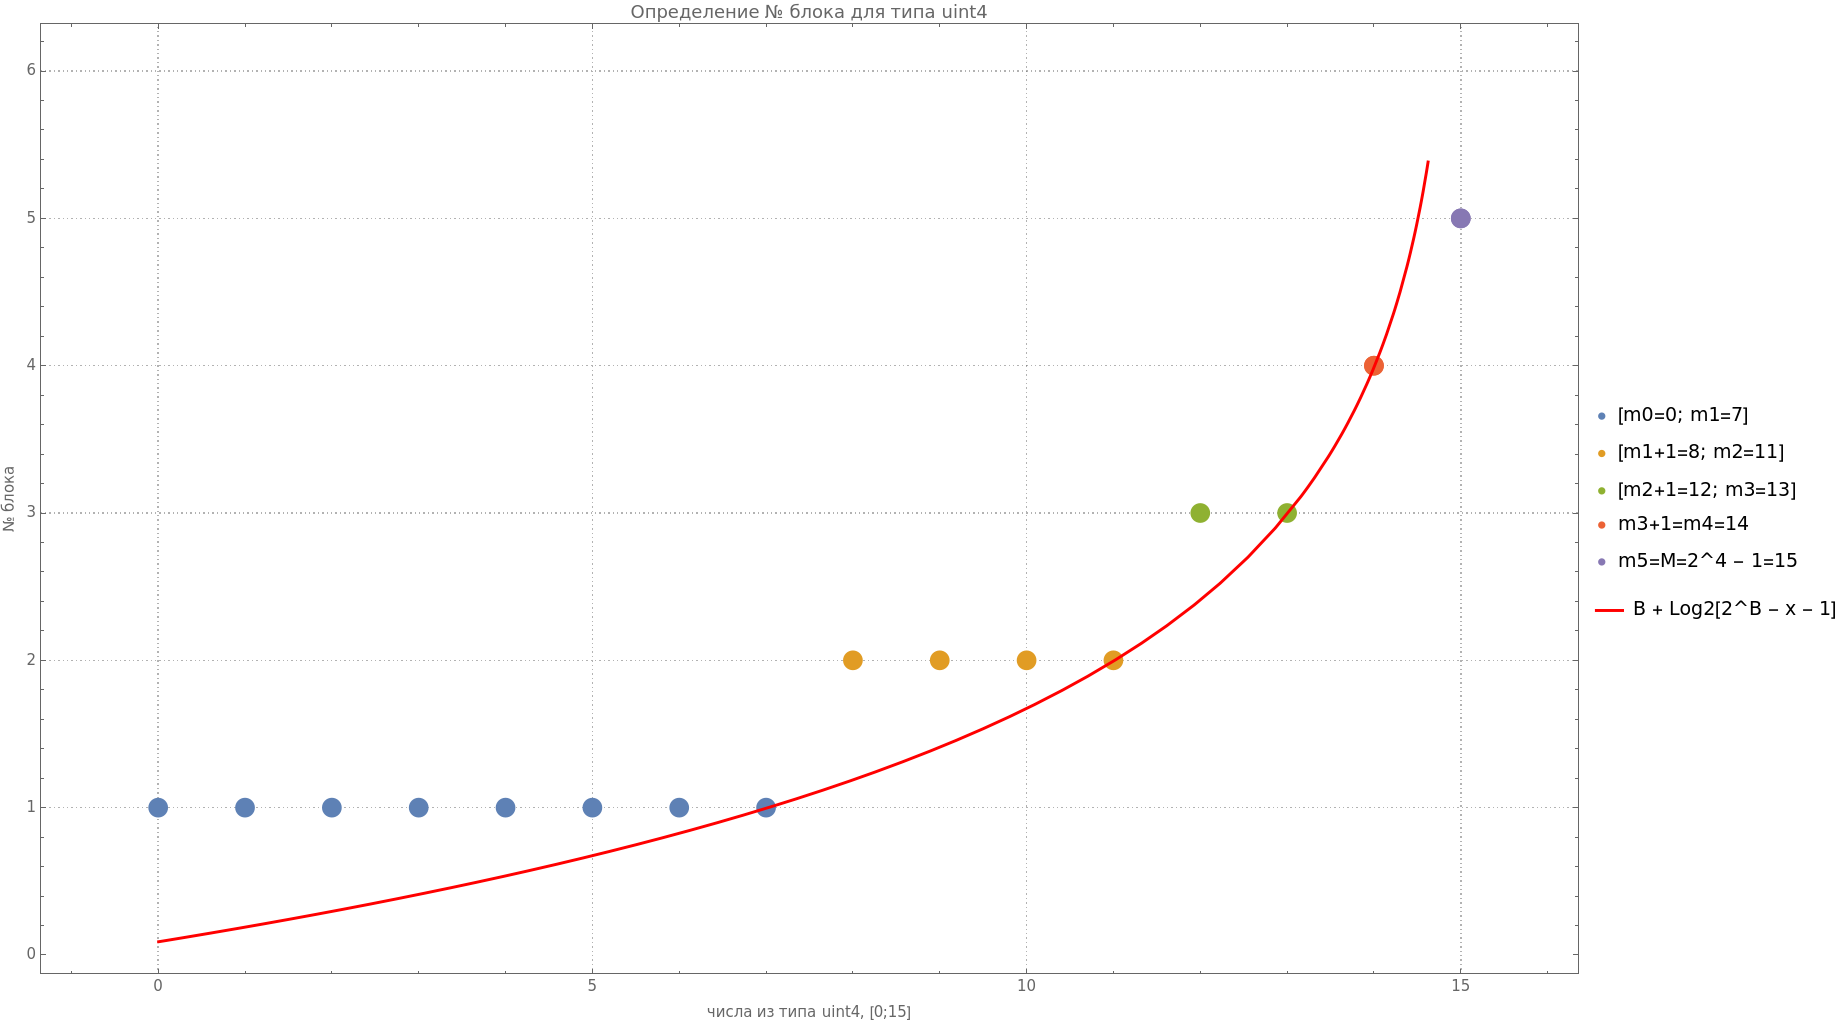
\includegraphics[width=1.0\textwidth]{../../resources/number_block_for_uint4.png}
    \caption{}
\end{figure}
 
Перед тем как об суждать сколько нам потребуется памяти и, как уйти от счётчиков, давайте реализуем сказанное в коде.

\section{Реализация способа с счётчиками в коде}

Чтобы иметь возможность задавать \texttt{B}, тем самым "выбирать"{} тип \texttt{uintB}, давайте просто считать, что типы элементов и счётчиков в нашей программе -- это \texttt{size_t}, причём будем предпологать, что \texttt{size_t} 64-битный. Конечно, НЕ следует использовать данные реализации где-либо кроме каких-то демонстрационных проектов. 

Рассмотрим \texttt{./solver_1/solution.hpp}:
\begin{minted}[breaklines=true]{cpp}
    size_t log2(size_t x);

class Stack {
private:
  // Количество бит для чисел в типе. Для unit4 равно4
  // для обычного unsigned int равно 32 может быть 64
  size_t B = 0;
  size_t M = 0;
  // Создаём вспомогательный вектор с счётчиками Подробнее читать в pdf.
  std::vector<size_t> count_elements;
  std::vector<size_t> stack;
  size_t max_value = 0; // текущий максимум стека
  // текущий id блока, которому принадлежит max_value
  size_t block_id = 0;

  size_t calculate_block_id(size_t value);

public:
  Stack(size_t B_, size_t length_);

  void push(size_t value);
  size_t pop();

  // Возвращает истинное значение добавленного элемента
  size_t back();
  // Возвращает значение последнего элемента в стеке, которое может быть
  // закодировано.
  size_t top();

  size_t max();
  size_t size();
  size_t capacity();
  bool is_empty();
};
\end{minted}

Из особенностей -- это \texttt{block_id}, чтобы не подсчитывать \texttt{id} блока для текущего максимума, который может часто повторяться, мы его запоминаем. (Поскольку отсчёт начинается \texttt{0}, то мы будем работать с \texttt{id}, а не номерами блока.) Рассмотрим \texttt{./solver_1/solution.cpp}
\begin{minted}[breaklines=true]{cpp}
  Stack::Stack(size_t B_, size_t length_)
  : B{B_},
    // Максимальное число для нашего типа 2^B  - 1 (для unit4 равное 15)
    M{(B == 64) ? ~0uz : (1uz << B) - 1uz}, count_elements(B_ + 1uz, 0uz) {

  stack.reserve(length_);
}
\end{minted}

В конструктуре по заданному \texttt{B_} создаём нужное количество счётчиков и инициализируем их нулями, а также вычисляем \texttt{M}, причём, чтобы избежать переполнения в \texttt{1uz << B} при \(B = 64\) мы рассматриваем этот случай отдельно. Очевидно, что при передаче \texttt{B} большего чем размер \texttt{size_t} мы получим UB. Чтобы при замерах не тратить время на увеличение вектора, мы можем сразу передать заданную длину \texttt{length_} и выполнить \texttt{reserve}.

\begin{minted}[breaklines=true]{cpp}
size_t log2(size_t x) {
  [[assume(x != 0)]];
  return std::bit_width(x) - 1; // bit_width вернёт int
  // см. https://en.cppreference.com/w/cpp/numeric/bit_width
}

size_t Stack::calculate_block_id(size_t value) {
  // Вычисляем какому из блоково принадлежит число value:
  if (value == M) {
    // Максимальное число мы обрабатываем отдельно
    return B; // последний из возможных id блока
  } else {
    // Поскольку value < M, то значит M - value != 0, поэтому законно использовать log2 с указанным assume
    return (B - 1uz - log2(M - value));
  }
}
\end{minted}
```

Реализация основных двух функций:
\begin{minted}[breaklines=true]{cpp}
void Stack::push(size_t value) {
  if (value <= max_value) {
  // В данном случае ни max_value, ни block_id не изменятся.
  // Увеличиваем количество элементов для блока, которому принадлежит
  // max_value.
  count_elements[block_id] += 1;
  stack.push_back(value);
  } else {
  // value > max_value, поэтому потребуется обновление max_value и возможно
  // block_id.
  size_t new_max_value = value;
  size_t new_block_id = calculate_block_id(new_max_value);
  if (new_block_id == block_id) {
    // Выполняем стандартное добавление, поскольку гарантировано не будет
    // переполнения.
    stack.push_back((value - max_value) + value); // 2*value - max_value
  } else {
    // Мы добавляем элемент из другого блока сохраняем старый max, как
    // элемент стека, чтобы при pop востановить его.
    stack.push_back(max_value);
  }
  count_elements[new_block_id] += 1;
  // Перезаписываем max_value и block_id
  max_value = new_max_value;
  block_id = new_block_id;
  }
}
\end{minted}
Заметим, поскольку изначально при пустом стеке \texttt{max_value = 0}, то случая добавления первого элемента корректен.
\begin{minted}[breaklines=true]{cpp}
size_t Stack::pop() {
  // Вызов pop для пустого контейнера приводит к неопределенному поведению.
  // Мы знаем текущий max_value, его block_id и верхний элемент стека,
  // кототрый может быть: предыдущим max, истинным добавленным значением,
  // значением, для определения предыдущего max.
  size_t element = stack.back();
  count_elements[block_id] -= 1;
  stack.pop_back();
  if (count_elements[block_id] == 0) {
   // Мы удаляем последний элемент для данного блока, то есть element --
   // это либо прошлый max, либо если block_id = 0, то значит мы удалили
   // последний элемент всего стека.
   if (block_id == 0) {
    // element -- последний элемент всего стека, а значит текущий max_value и
    // есть сам элемент. Поскольку нам надо изменить max_value в изначальное
    // значение, равное 0, то сохраним текущее значение в element
    element = max_value;
    max_value = 0;
    return element;
   } else {
    // element -- прошлый max, а возвращаемый элемент -- это текущий max.
    size_t res = max_value;
    max_value = element;
    block_id = calculate_block_id(element);
    return res;
   }
  } else {
   // возвращаем не последний элемент из блока
   if (element <= max_value) {
    // element -- истинное добавленное значение
    return element;
   } else {
    // element -- значение, которое будет использоваться, для вычисления
    // прошлого max_value, а текущее max_value -- это истинное добавленное
    // значение,
    size_t res = max_value;
    // востановим прошлый максимум по формуле 2 * max_value - element;
    // Чтобы не было переполнения в промежуточных шагах:
    size_t diff = element - max_value;
    // последнее корректно, так как в случае element > max_value

    // (max_value - diff =  max_value - (element - max_value) = 2*max_value -
    // element)
    max_value = max_value - diff;
    return res;
   }
  }
}
\end{minted}
\begin{minted}[breaklines=true]{cpp}
// Возвращает истинное значение добавленного элемента
size_t Stack::back() {
  // Вызов back для пустого контейнера вызывает неопределенное поведение.
  size_t element = stack.back();
  if (count_elements[block_id] == 1) {
    // Если в блоке всего одно число, значит текущий max_value
    // и есть последний элемент в массиве
    return max_value;
  } else {
    // в блоке больше чем одно число
    if (element <= max_value) {
      // element -- истинное добавленное значение
      return element;
    } else {
      // element -- значение, которое будет использоваться, для вычисления
      // прошлого max_value, а текущее max_value -- это истинное добавленное
      // значение,
      return max_value;
    }
  }
}
\end{minted}

Остальные методы -- это просто вызовы методов `vector`.
\begin{minted}[breaklines=true]{cpp}
// Возвращает значение последнего элемента в стеке, которое может быть
// закодировано.
size_t Stack::top() {
  // Вызов back для пустого контейнера вызывает неопределенное поведение.
  return stack.back();
}

size_t Stack::max() {
  // Вызов max для пустого контейнера возвращает 0.
  // Но не стоит этого делать!
  return max_value;
}

size_t Stack::size() { return stack.size(); }
size_t Stack::capacity() { return stack.capacity(); }

bool Stack::is_empty() { return stack.empty(); }
\end{minted}

\section{Тестирование и замеры}

Способ тестирования и как можно добавлять свои собственные тестовые данные можно найти в \texttt{tests.md}. Корректность по времени очевидна из кода, но также были сделаны замеры при помощи \texttt{google/benchmark}. 

Правильно и с большой точностью измерить скорость малых фрагментов кода -- довольно сложная задача, требующая много времени. Приведённые измерения не претендуют на это. Они скорее являются чем-то вроде: <<А давайте много раз выполним \texttt{push} в нашу реализацию стека, в реализацию стека с \(O(n)\) дополнительной памятью и в голый \texttt{vector}, а затем посмотрим на значения друг относительно друга. Если разрыв будет не большим, то значит всё хорошо, если большим и будет зависимость от количества элементов в стеке, то значит, что-то пошло не так. Повторим аналогичное для \texttt{pop} и \texttt{back}>>, то есть основная задача -- это показать независимость скорости выполнения операций относительно количества элементов в стеке.

Я также добавил специальные команды из \texttt{google/benchmark}, которые должны предотвратить оптимизацию \texttt{push} и других команд. (Но это не точно, поскольку я не специалист в использование этой библиотеки и не исследовал выходной код. Любые улучшения я срадостью почитаю.) 

Генератор для случайных чисел везде MT1997. Распределение -- равномерное с \(0\) и \(2^B - 1\).

В \texttt{./src/solver_1/benchmarks/benchmark_1.cpp}
\begin{minted}[breaklines=true]{cpp}
static void BM_stack_random_push(benchmark::State &state) {
  size_t data_size = state.range(0);
  std::vector<size_t> data;
  data.reserve(data_size);

  auto now = std::chrono::high_resolution_clock::now();
  std::mt19937 generator(now.time_since_epoch().count());
  std::uniform_int_distribution<size_t> distribution(0, IMAX);
  for (size_t i = 0; i < data_size; ++i) {
    data.emplace_back(distribution(generator));
  }

  Stack stack(B, data_size);
  for (auto _ : state) {
    // Этот код замеряем
    for (size_t i = 0; i < data_size; ++i) {
      size_t value = data[i];
      stack.push(value);
      benchmark::DoNotOptimize(value);
      benchmark::ClobberMemory();
    }
  }
}
\end{minted}

Здесь мы добавляем случайные данные. Очевидно, что если мы сразу добавим большое число, то текущий максимум будет большим, а значит последующие числа уже будут добавляться без вычисления \texttt{id} блока, без выполнения преобразования \(2\cdot v - m\), а просто будут добавляться, как в обычный вектор.

Поэтому в \texttt{./src/solver_1/benchmarks/benchmark_2.cpp} мы уже будем добавлять элементы последовательно от \(0\) до значений близких к \(2^B- 1\) с определённым шагом. 

В \texttt{./src/solver_1/benchmarks/benchmark_3.cpp}
\begin{minted}[breaklines=true]{cpp}
static void BM_stack_random_back_pop(benchmark::State &state) {
  size_t data_size = state.range(0);

  auto now = std::chrono::high_resolution_clock::now();
  std::mt19937 generator(now.time_since_epoch().count());
  std::uniform_int_distribution<size_t> distribution(0, IMAX);

  Stack stack(B, data_size);
  for (auto _ : state) {
    state.PauseTiming();
    for (size_t i = 0; i < data_size; ++i) {
      stack.push(distribution(generator));
    }
    state.ResumeTiming();
    // Этот код замеряем
    size_t value_back = 0;
    size_t value_pop = 0;
    for (size_t i = 0; i < data_size; ++i) {
      value_back = stack.back();
      benchmark::DoNotOptimize(value_back);
      value_pop = stack.pop();
      benchmark::DoNotOptimize(value_pop);
      benchmark::ClobberMemory();
    }
  }
} 
\end{minted}
мы сперва генерируем случайные данные, затем заполняем ими стек, а после чего измеряем время вызова двух команд \texttt{stack.back();}, который должен вернуть нам истинное значение, которое было добавлено в стек (не преобразованное по формуле, а именно то, что мы указывали в \texttt{push}), а также \texttt{stack.pop();}. Конечно, для нашего стека получается лишняя работа, так как \texttt{value_back = value_pop} и правильней было бы переписать \texttt{pop}, чтобы он отвечал лишь за удаление элемента, но ... "ну и ладно ну и пожалуйста". (В оправдание могу сказать лишь то, что и \texttt{pop}, и \texttt{back} должны работать за $O(1)$, а поэтому относительно \texttt{vector} и эталонного стека, с которым мы сравниваем мы должны будем увидеть лишь константное изменение. А поскольку основная цель этих замеров, показать независимость от количества элементов в стеке, то всё не так страшно.)

\texttt{benchmark_1} и \texttt{benchmark_2} был запущен с \texttt{--benchmark_repetitions=25}, а \texttt{benchmark_3} с \texttt{10}. Для получения результатов на первые два теста ушло $15$ минут реального времени, а для последнего $23$ на процессоре i7-8750H CPU при зафиксированной частоте работы в $3000$ MHz. Полный выход измерений можно найти в `results`.

\subsection{Наглядные результаты для solver_1:}

Общее время выполнения измерения. Поскольку мы измеряям цикл \texttt{for} целиком, то время увеличивается линейно:
\begin{figure}[H]
  \centering
  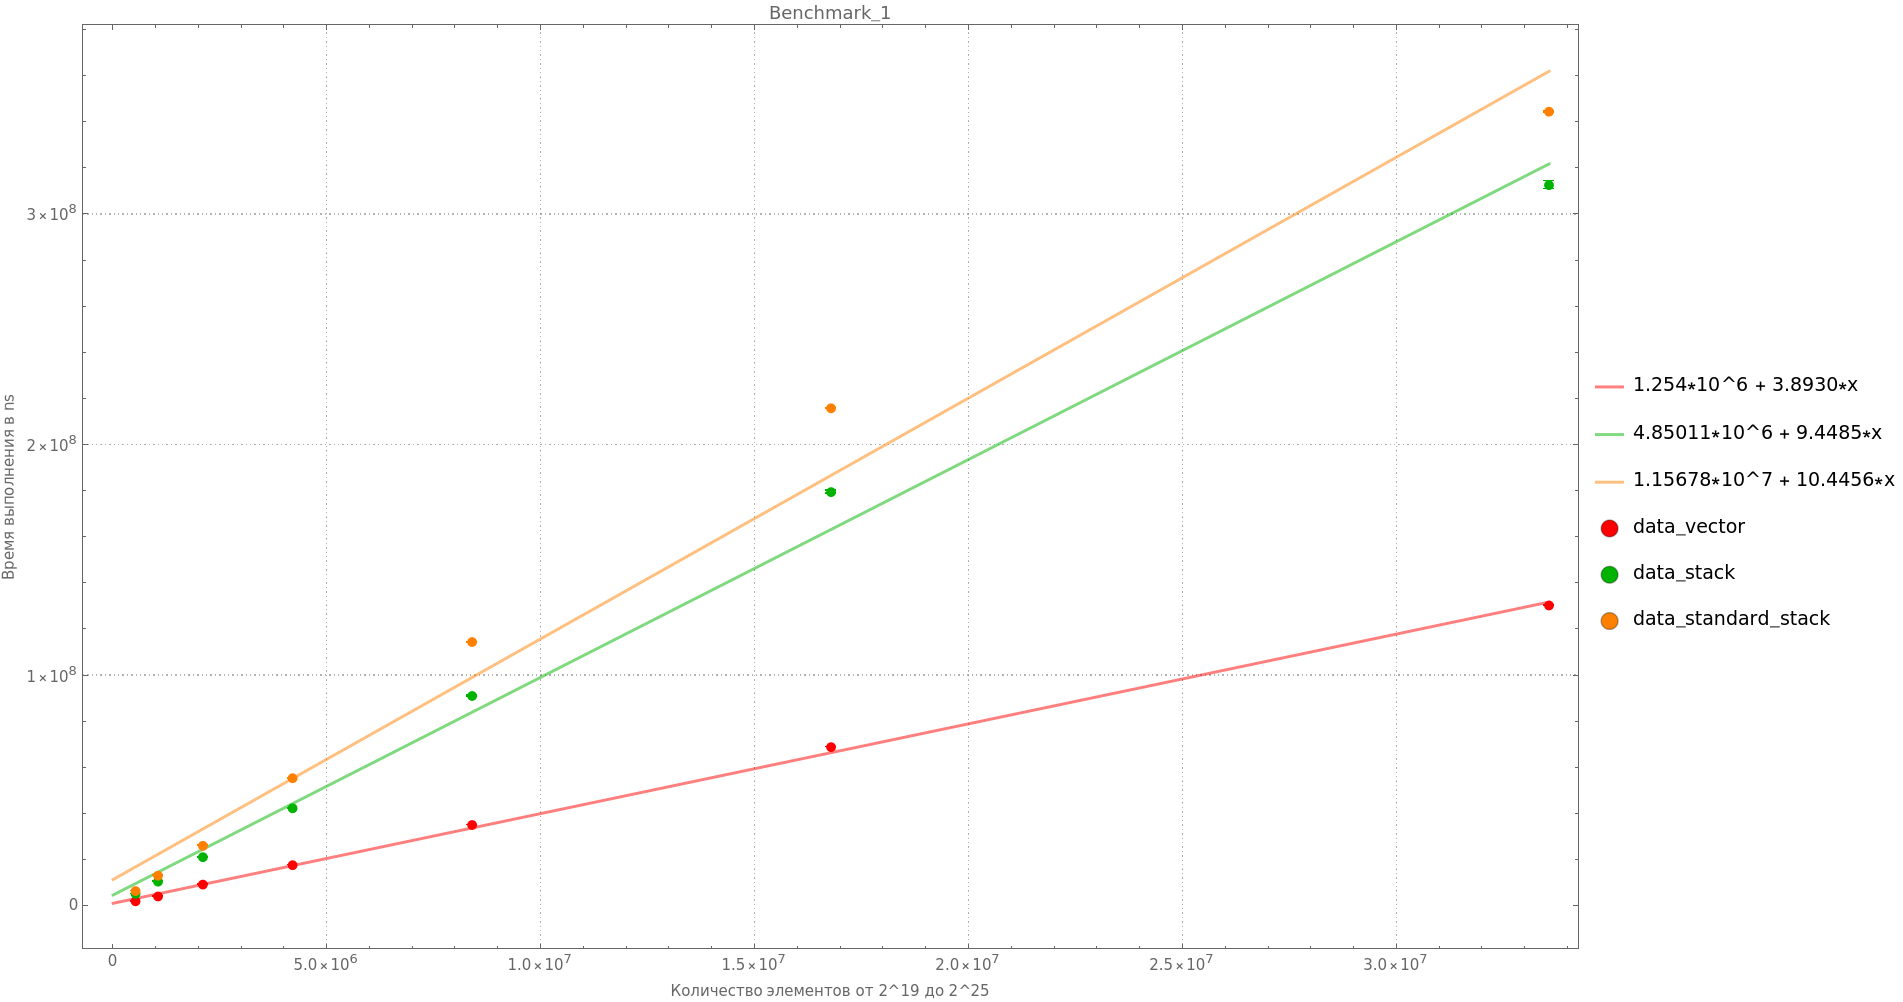
\includegraphics[width=1.0\textwidth]{../../resources/benchmark_1_1.png}
  \caption{}
\end{figure}
если мы разделим общее время выполнения измерения на количество добавленных элементов, то получим примерное время добавления одного элемента \texttt{push}:
\begin{figure}[H]
  \centering
  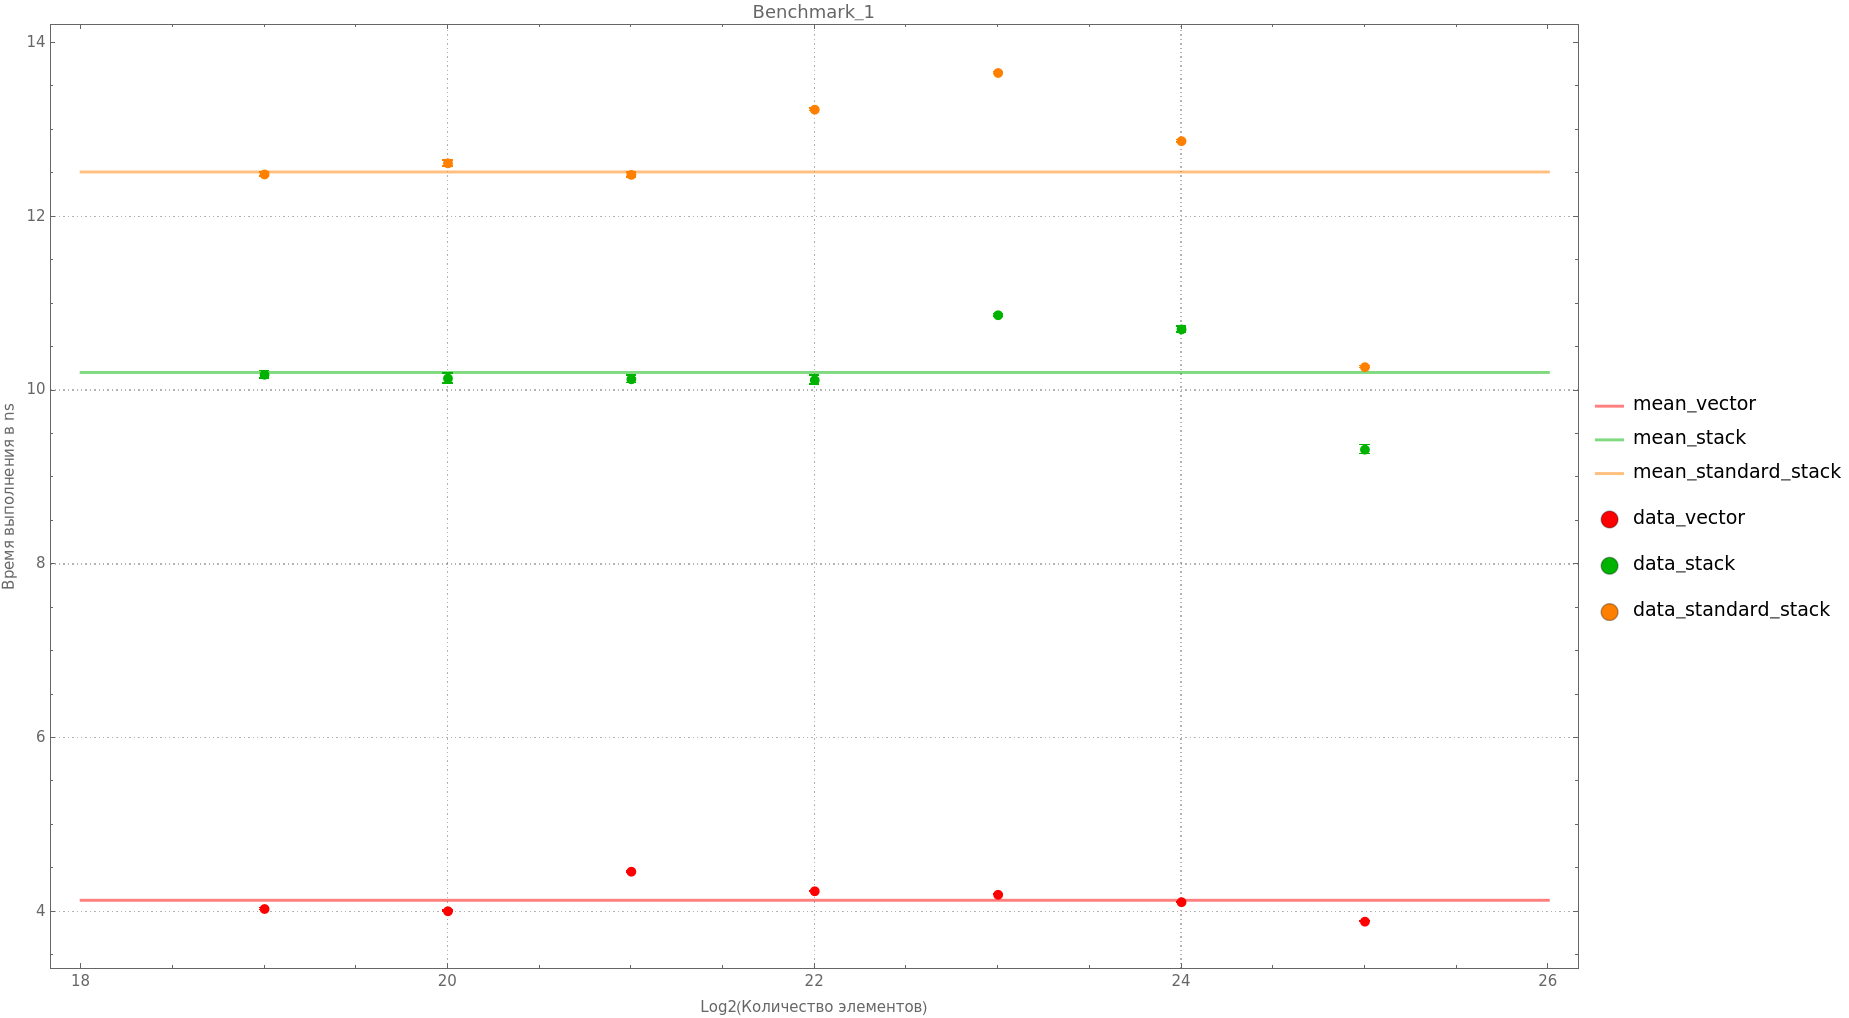
\includegraphics[width=1.0\textwidth]{../../resources/benchmark_1_2.png}
  \caption{}
\end{figure}

Для каждой структуры: \texttt{vector, stack, standard_stack (из \texttt{standard_solution.hpp})}:
\begin{figure}[H]
  \centering
  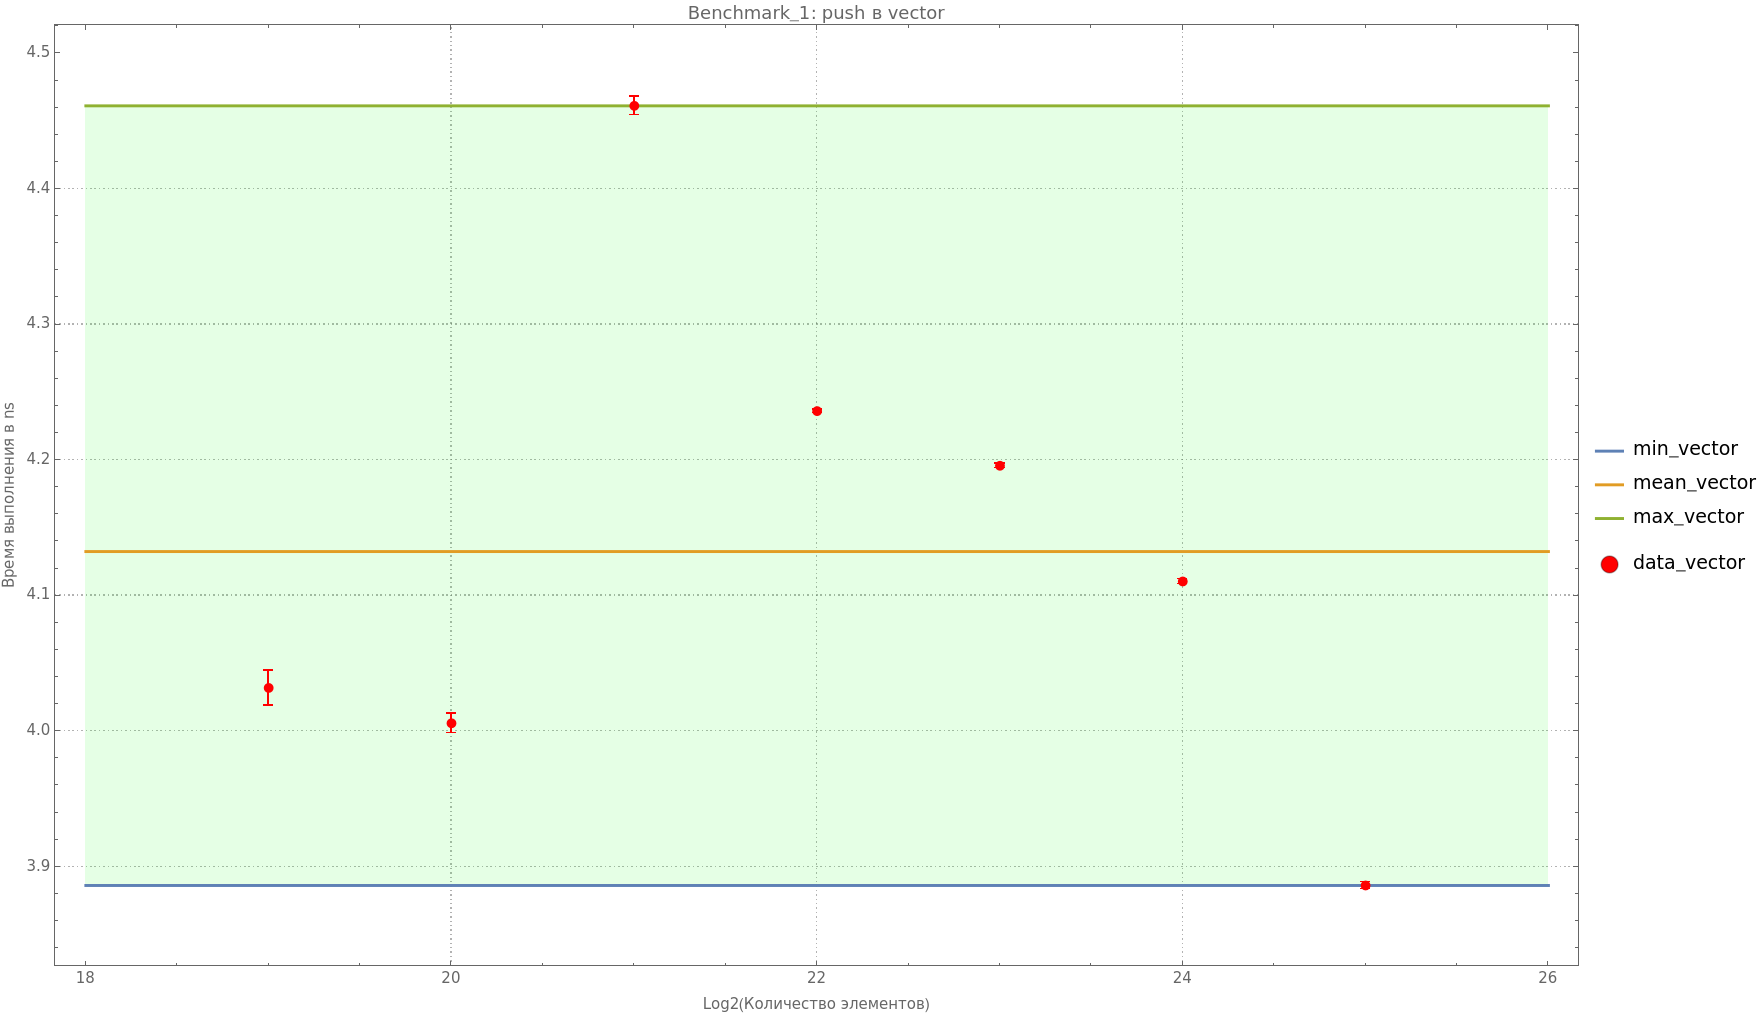
\includegraphics[width=1.0\textwidth]{../../resources/benchmark_1_3.png}
  \caption{}
\end{figure}
\begin{figure}[H]
  \centering
  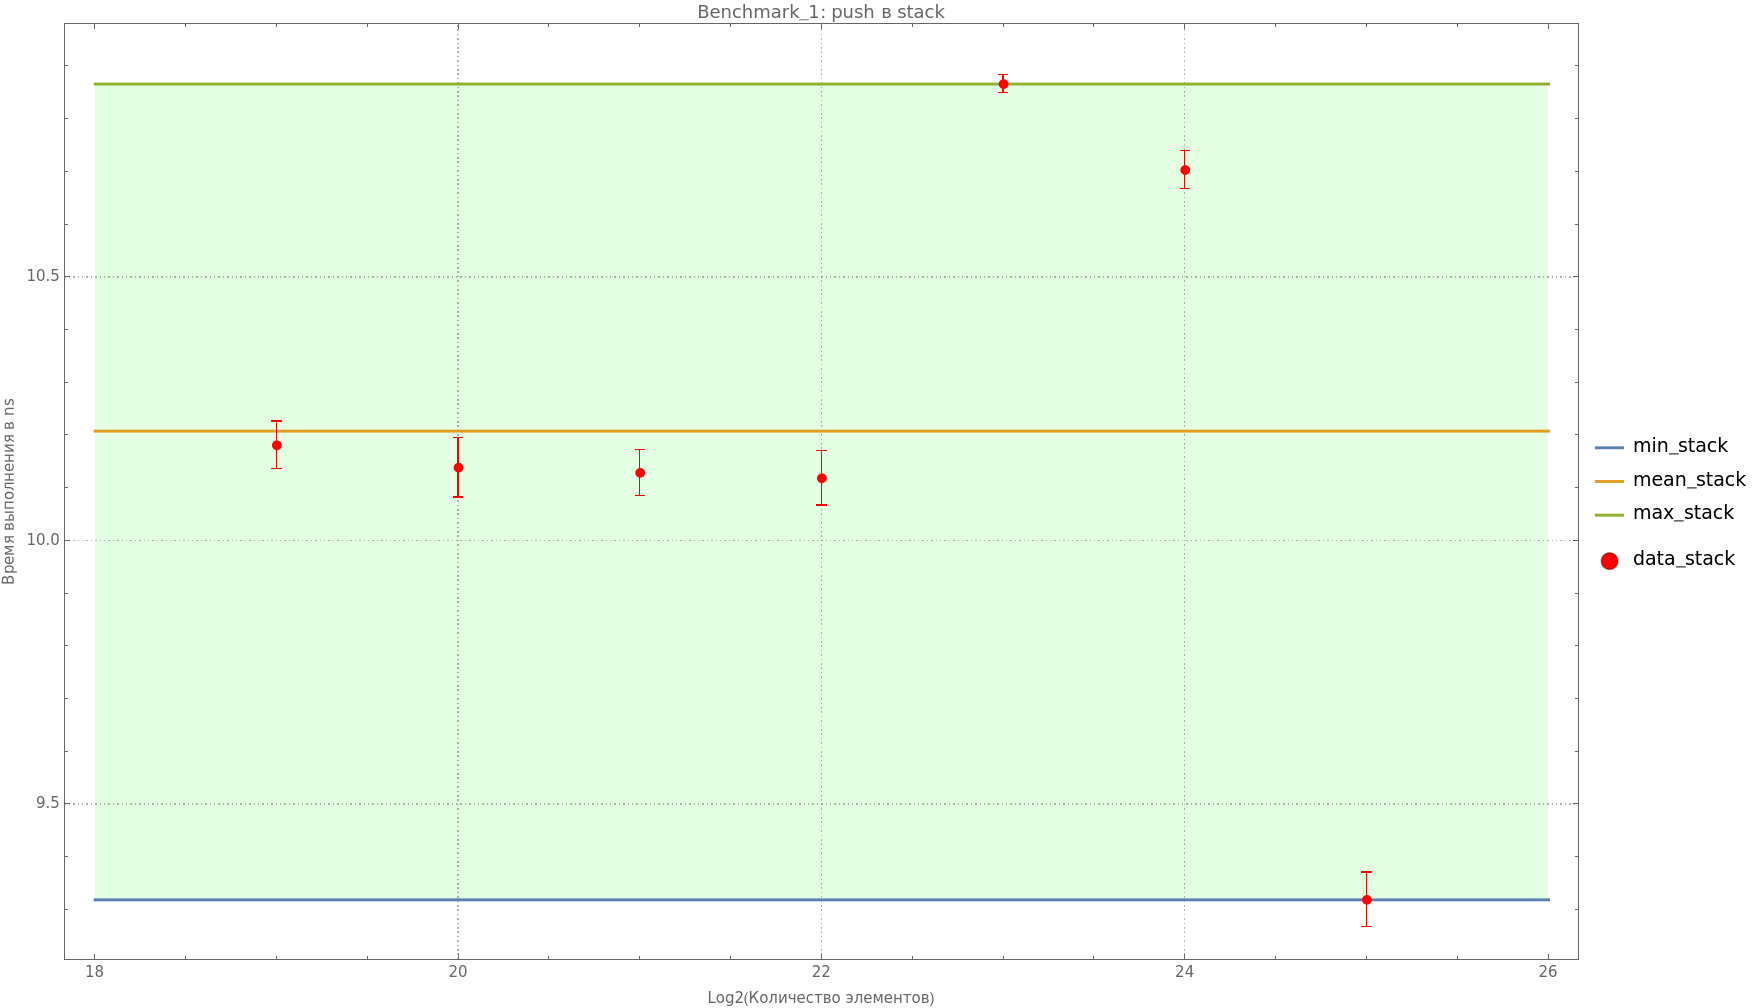
\includegraphics[width=1.0\textwidth]{../../resources/benchmark_1_4.png}
  \caption{}
\end{figure}
\begin{figure}[H]
  \centering
  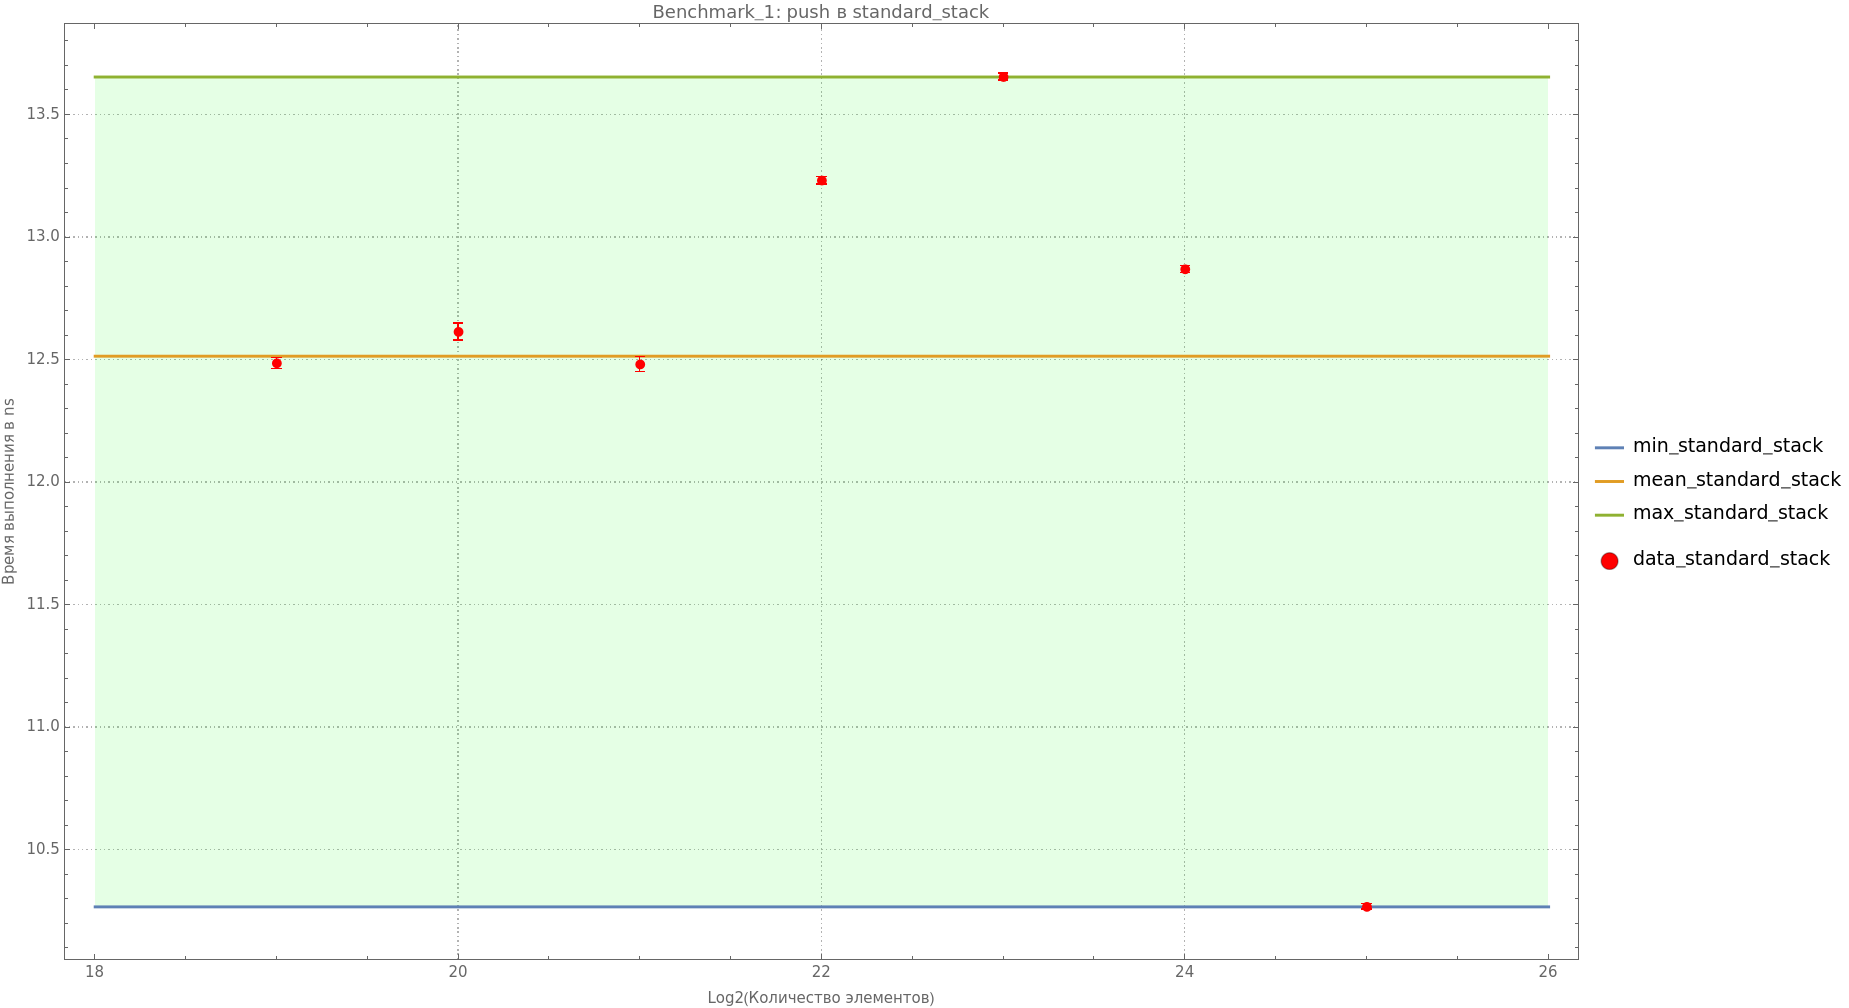
\includegraphics[width=1.0\textwidth]{../../resources/benchmark_1_5.png}
  \caption{}
\end{figure}

Аналогично для \texttt{benchmark_2}:
\begin{figure}[H]
  \centering
  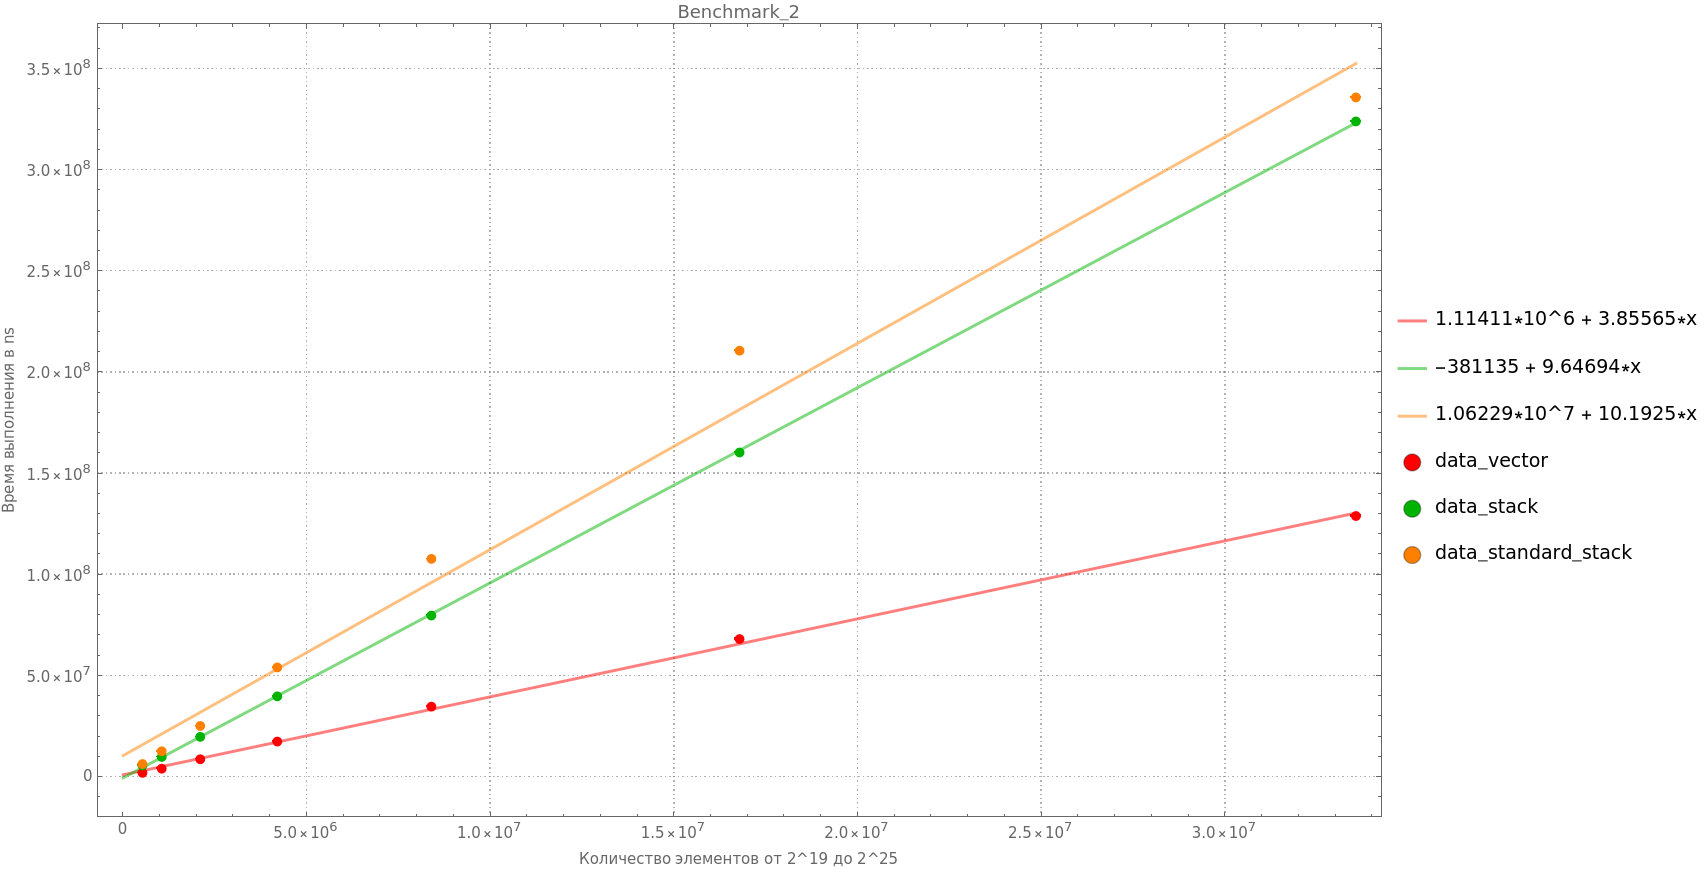
\includegraphics[width=1.0\textwidth]{../../resources/benchmark_2_1.png}
  \caption{}
\end{figure}
\begin{figure}[H]
  \centering
  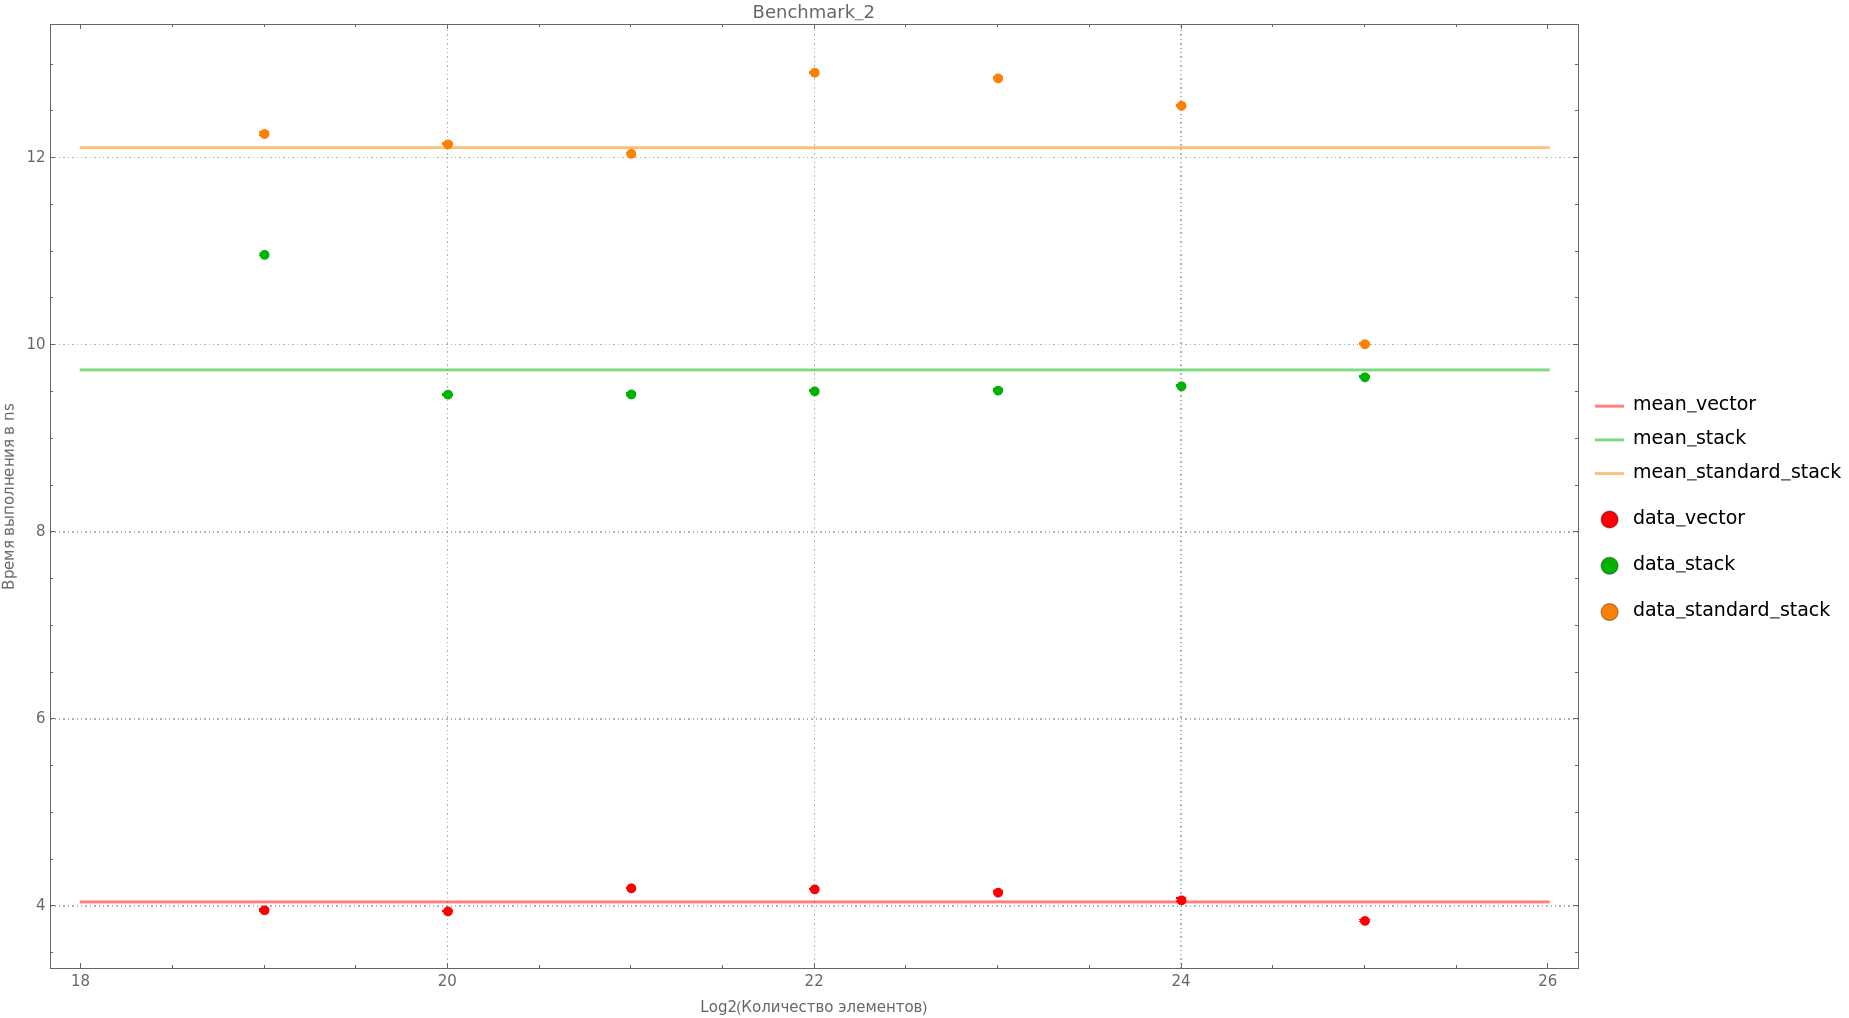
\includegraphics[width=1.0\textwidth]{../../resources/benchmark_2_2.png}
  \caption{}
\end{figure}
\begin{figure}[H]
  \centering
  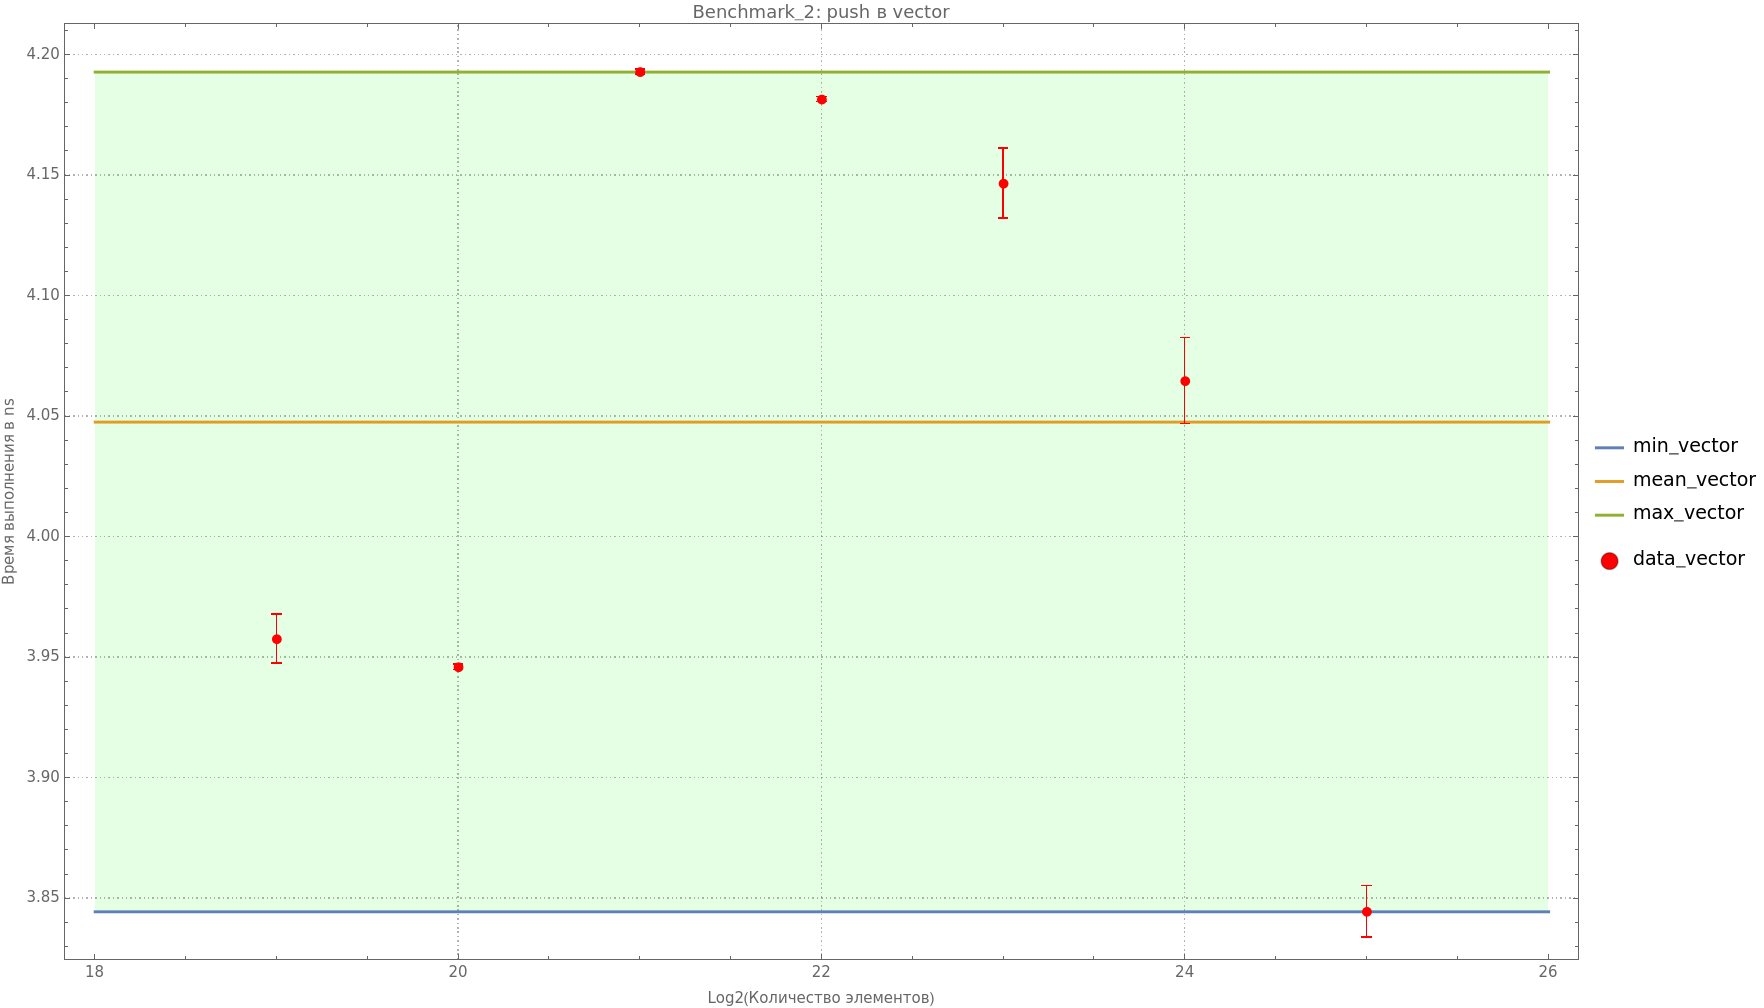
\includegraphics[width=1.0\textwidth]{../../resources/benchmark_2_3.png}
  \caption{}
\end{figure}
\begin{figure}[H]
  \centering
  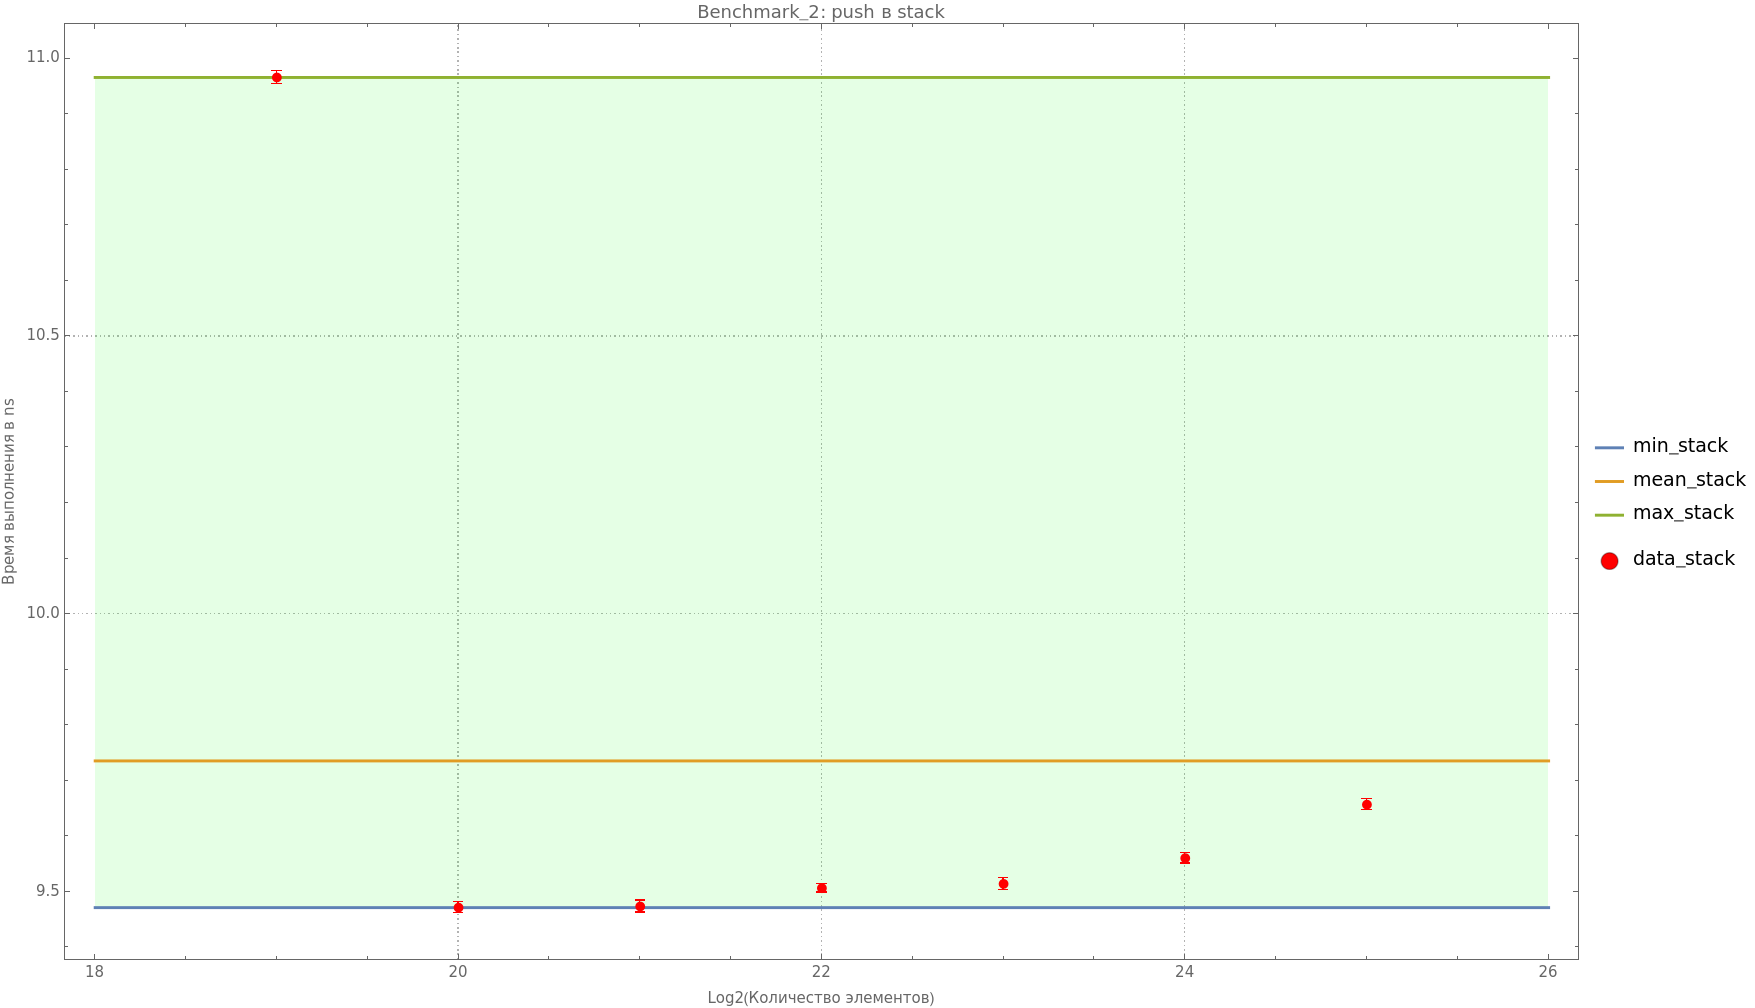
\includegraphics[width=1.0\textwidth]{../../resources/benchmark_2_4.png}
  \caption{}
\end{figure}
\begin{figure}[H]
  \centering
  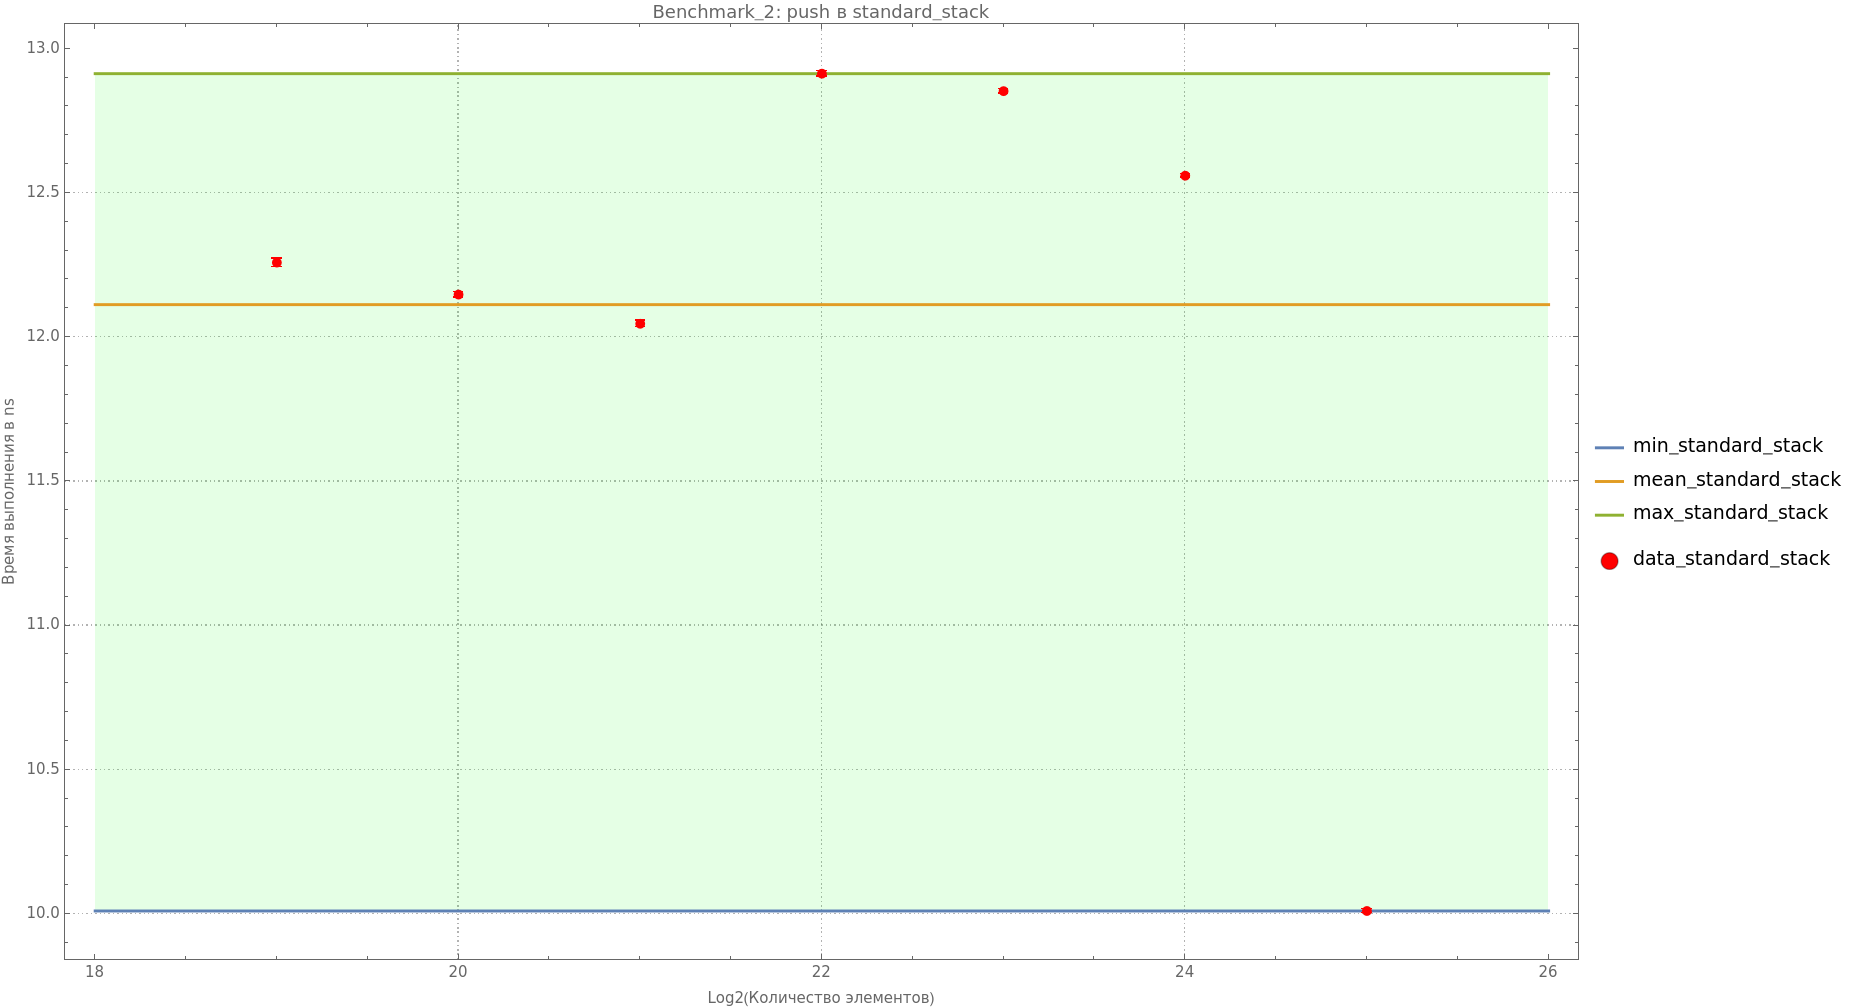
\includegraphics[width=1.0\textwidth]{../../resources/benchmark_2_5.png}
  \caption{}
\end{figure}

Аналогично для \texttt{benchmark_3}:
\begin{figure}[H]
  \centering
  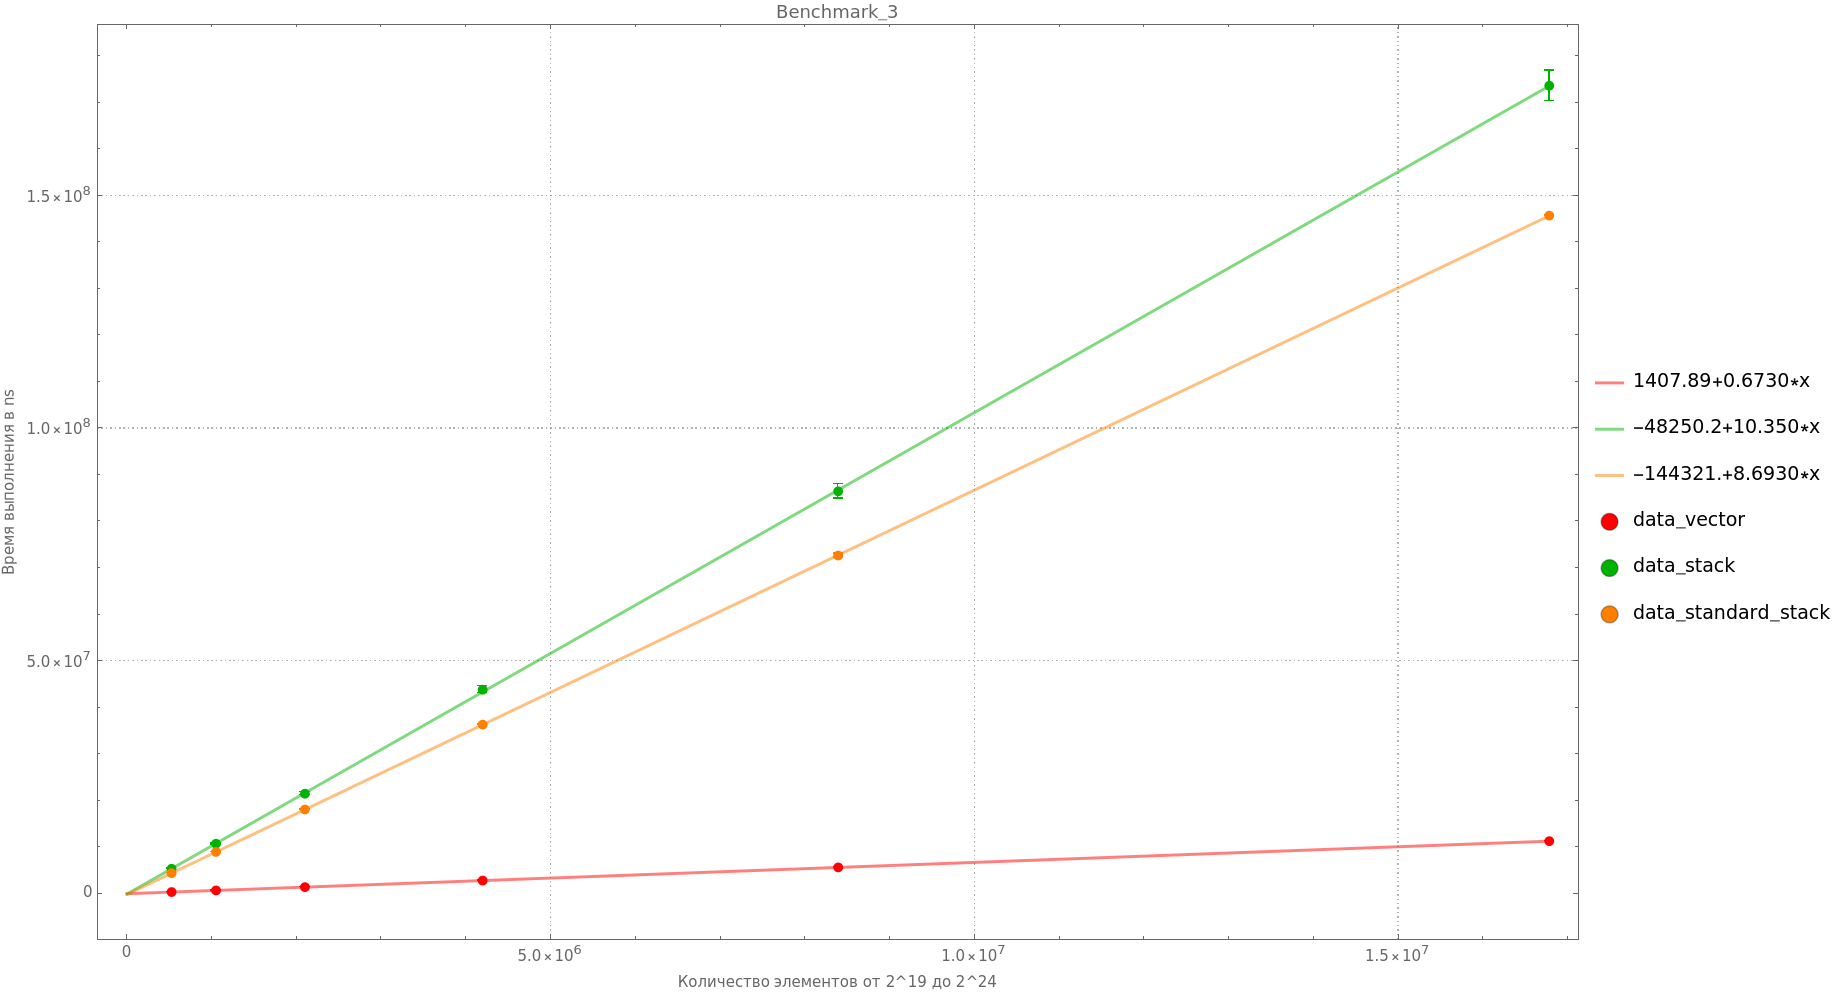
\includegraphics[width=1.0\textwidth]{../../resources/benchmark_3_1.png}
  \caption{}
\end{figure}
\begin{figure}[H]
  \centering
  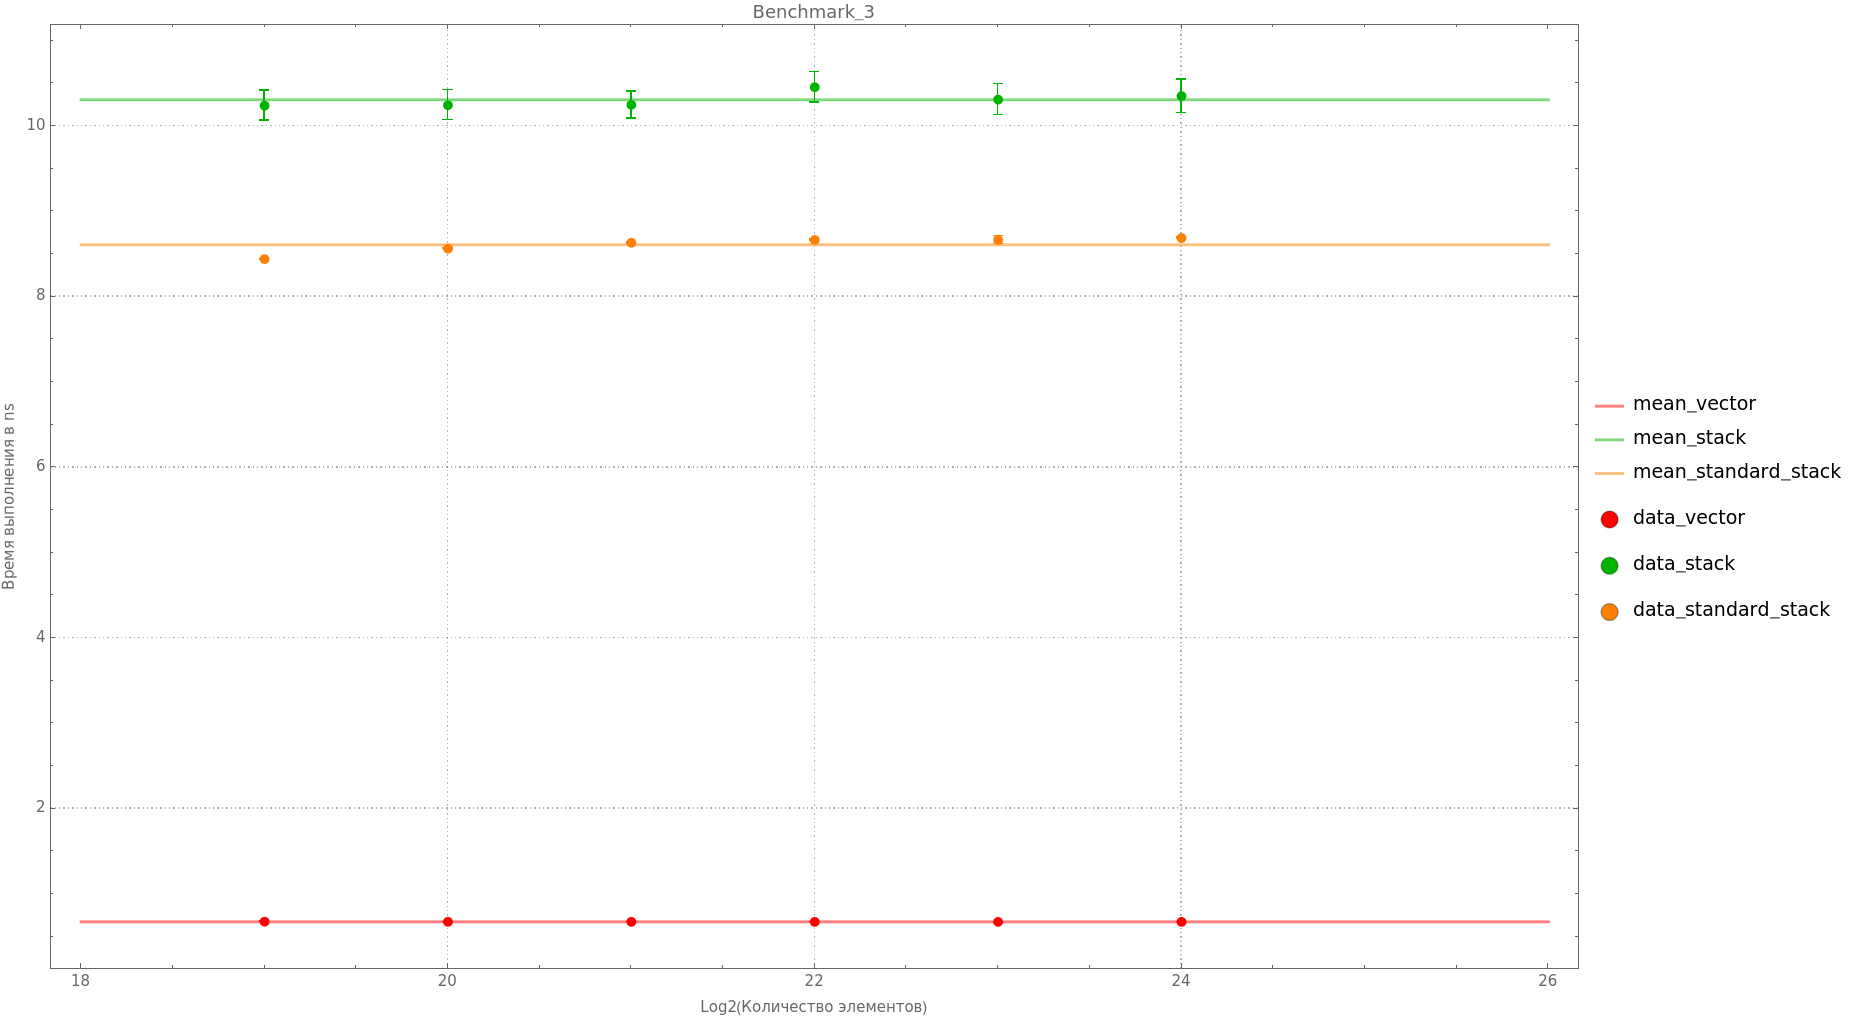
\includegraphics[width=1.0\textwidth]{../../resources/benchmark_3_2.png}
  \caption{}
\end{figure}
\begin{figure}[H]
  \centering
  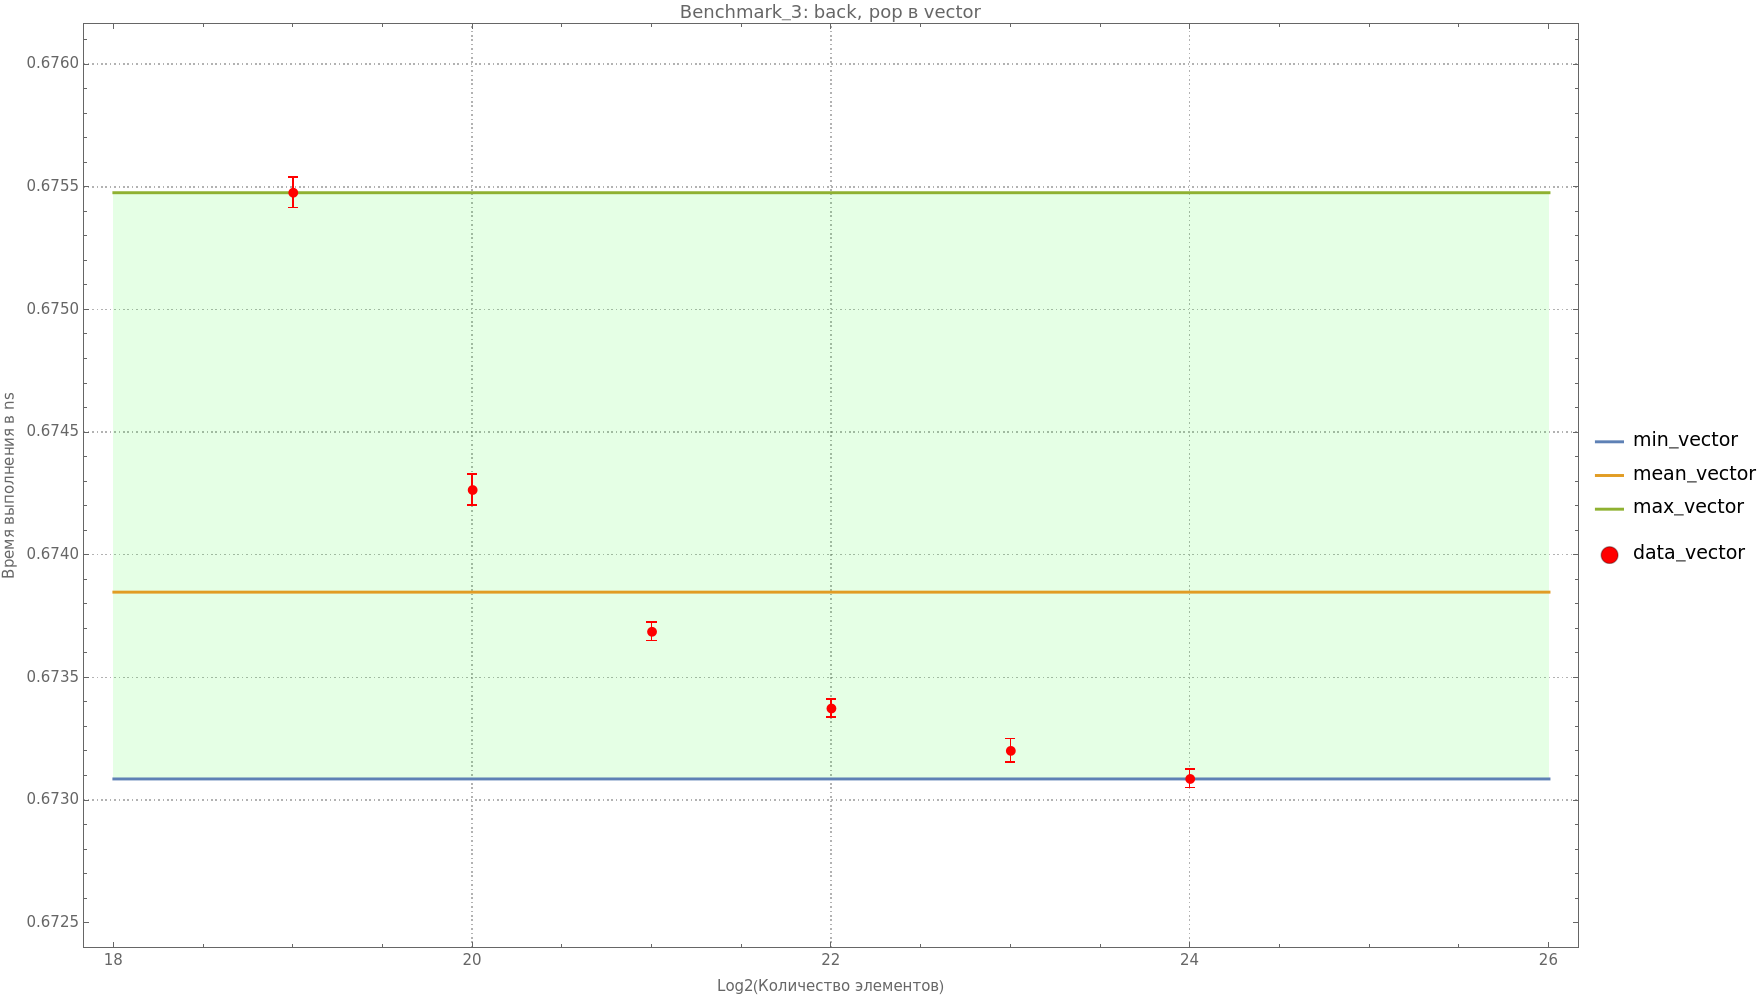
\includegraphics[width=1.0\textwidth]{../../resources/benchmark_3_3.png}
  \caption{}
\end{figure}
\begin{figure}[H]
  \centering
  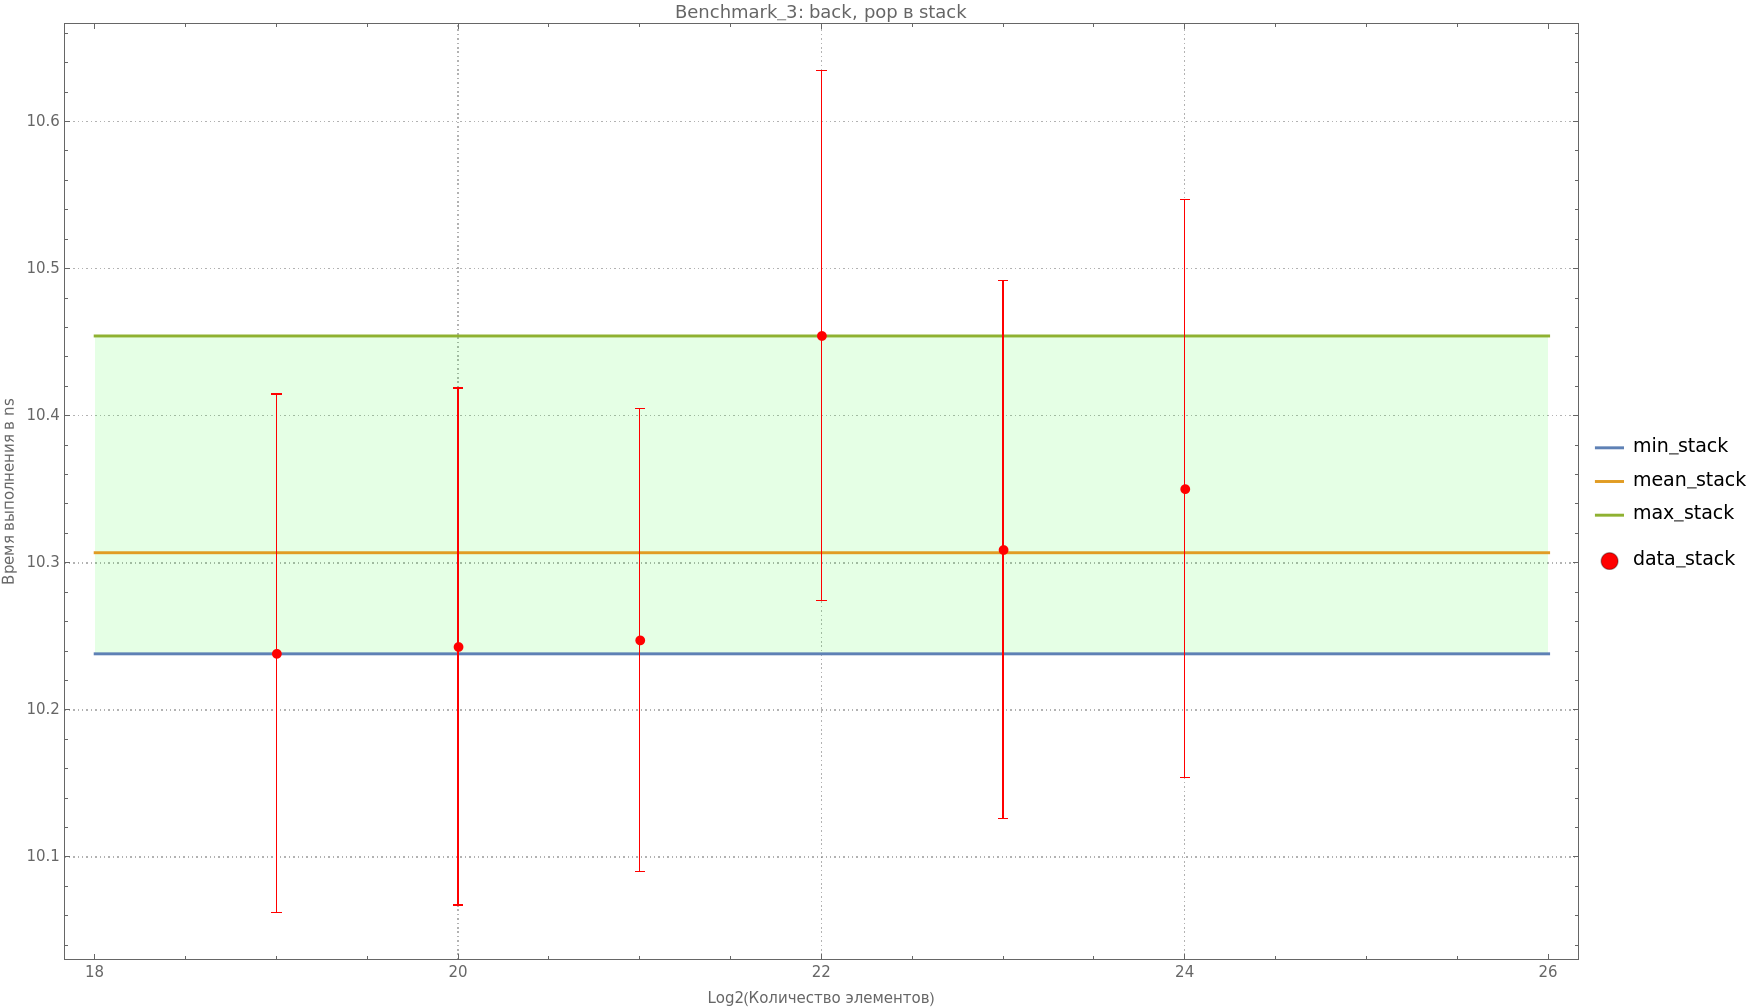
\includegraphics[width=1.0\textwidth]{../../resources/benchmark_3_4.png}
  \caption{}
\end{figure}
\begin{figure}[H]
  \centering
  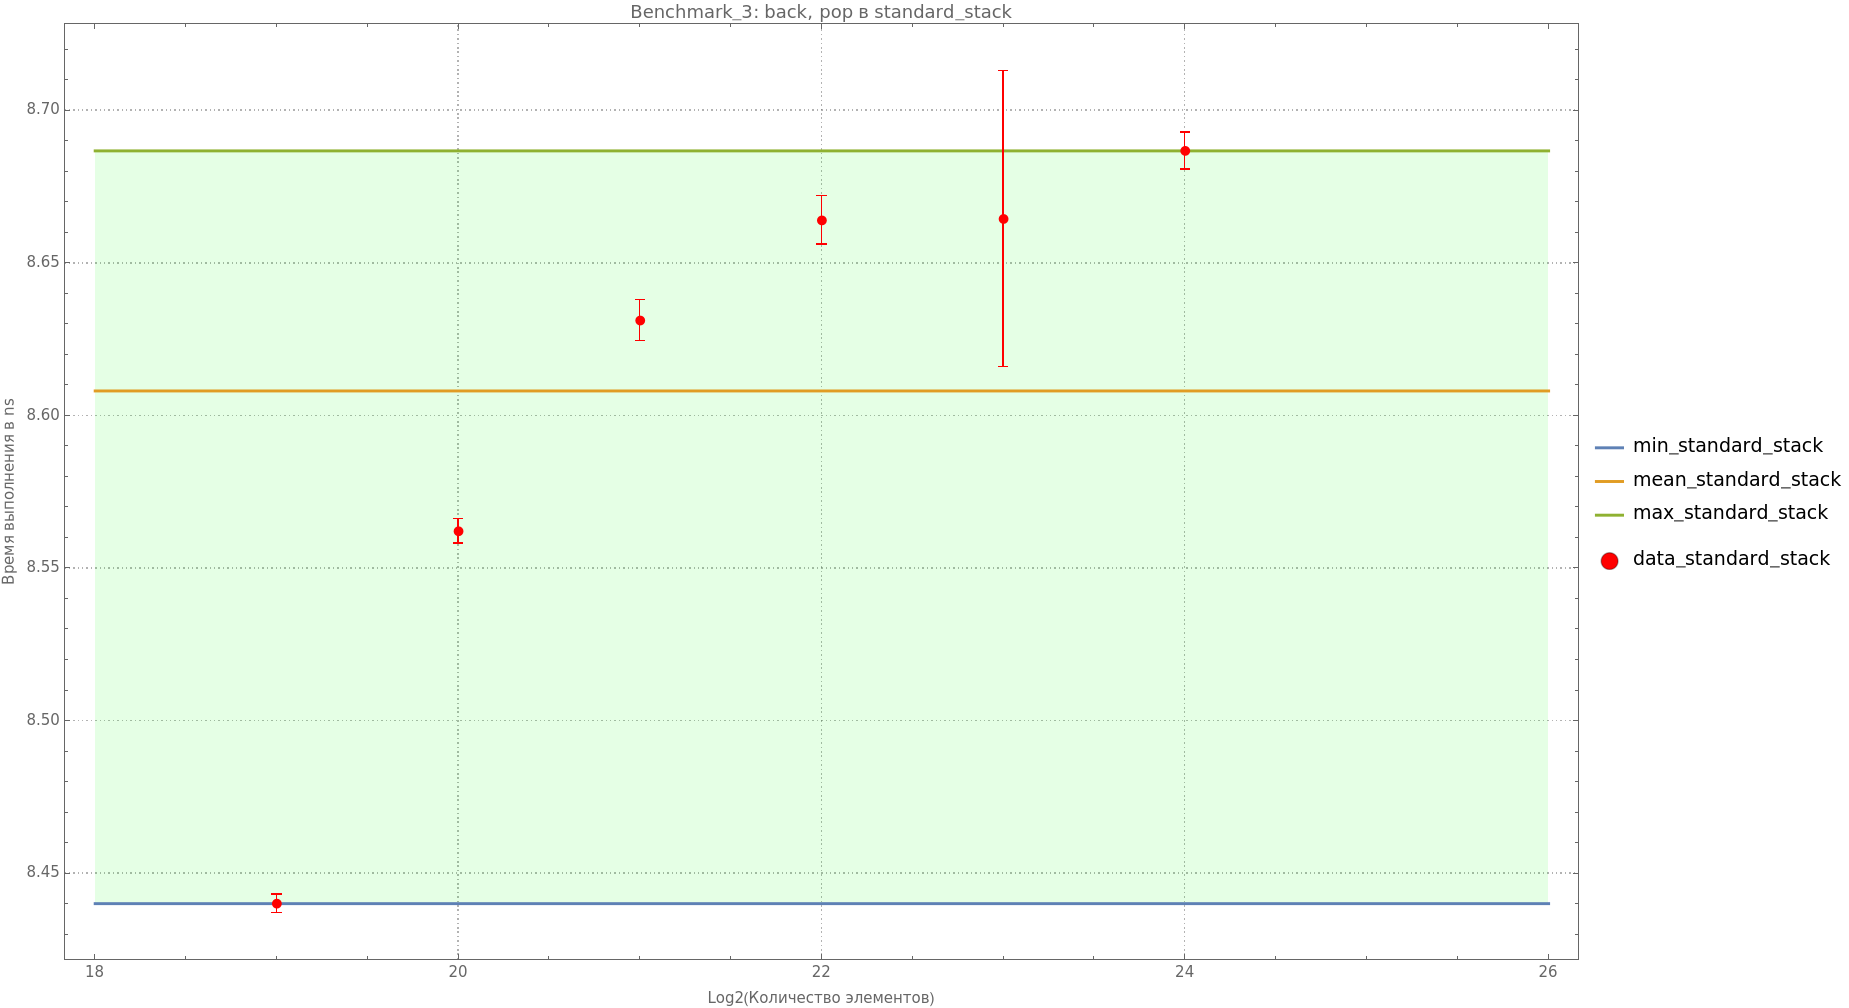
\includegraphics[width=1.0\textwidth]{../../resources/benchmark_3_5.png}
  \caption{}
\end{figure}

\section{Недочёты приведённого решения}

В приведённом выше методе мы дополнительно используем \texttt{B+1} счётчиков, размер которых зависит от количества элементов. В худшем случае все элементы будут складываться в один счётчик, а поэтому размер счётчика должен быть таким, чтобы суметь уместить все элементы. Соответственно количество бит для счётчика будет \(\log_2(N)\), где \(N\) -- количество элементов в стеке.
\begin{mdframed}[style=mdfStyleCode]%
    \begin{remark}\rm%
    Мы ещё вернёмся к обсуждению наличия счётчика в стеке.
\end{remark}
\end{mdframed}

\section{Решение для стека на односвязном списке}

А сейчас для полноты картины давайте рассмотрим классическую реализацию стека на односвязном списке (\texttt{./src/default_stack_list/default_stack_list.hpp}). Для наглядности и без использования шаблонов, давайте используем \verb|using elem_t = size_t;| 
\begin{minted}[breaklines=true]{cpp}
using elem_t = size_t;

// Определение структуры узла односвязного списка
struct Node {
  elem_t data;
  Node *next;
  Node(elem_t data_, Node *next_ = nullptr) : data{data_}, next{next_} {}
};

// Определение класса стека
class Default_Stack {
private:
  Node *top; // Верхний элемент стека

public:
  // Конструктор
  Default_Stack() : top(nullptr) {}

  // Деструктор
  ~Default_Stack();

  // Проверка на пустоту стека
  bool is_empty() const;

  // Добавление элемента в стек (пуш)
  void push(elem_t value);

  // Удаление элемента из стека
  elem_t pop();

  // Получение верхнего элемента стека без удаления (пик)
  elem_t back() const;
};
\end{minted}

Реализация (\verb|default_stack_list.cpp|) также очевидна:
\begin{minted}[breaklines=true]{cpp}
Default_Stack::~Default_Stack() {
  while (top) {
    Node *temp = top;
    top = top->next;
    delete temp;
  }
}
  
bool Default_Stack::is_empty() const { return top == nullptr; }

void Default_Stack::push(elem_t value) { top = new Node(value, top); }

elem_t Default_Stack::pop() {
  elem_t value = top->data;
  Node *temp = top;
  top = top->next;
  delete temp;
  return value;
}

elem_t Default_Stack::back() const { return top->data; }
\end{minted}

Как используя эту стандартную реализацию мы можем её видоизменить и добавить метод \texttt{max()}?

Аналогично, использя прошлую идею с разбиением на блоки. Только теперь в полях \texttt{Stack} мы будем хранить не один \texttt{Node *top}, а \texttt{B + 1} такой указатель (\texttt{solver_2/solution.hpp}):
\begin{minted}[breaklines=true]{cpp}
// Определение класса стека
class Stack {
private:
  // Количество бит для чисел в типе. Для unit4 равно4
  // для обычного unsigned int равно 32 может быть 64
  elem_t B = 0;
  elem_t M = 0;

  Node **stacks; // B + 1 будующих стеков

  elem_t max_value = 0; // текущий максимум стека
  // текущий id блока, которому принадлежит max_value
  elem_t block_id = 0;

  elem_t calculate_block_id(elem_t value);

public:
  // Конструктор
  Stack(elem_t B);

  // Деструктор
  ~Stack();

  // Проверка на пустоту стека
  bool is_empty(elem_t id) const;
  bool is_all_empty() const;

  elem_t max() const;

  // Добавление элемента в стек (пуш)
  void push(elem_t value);

  // Удаление элемента из стека
  elem_t pop();

  // Получение верхнего элемента стека без удаления (пик)
  elem_t back() const;
};
\end{minted}

Приведём здесь лишь реализацию основных методов (полный код можно найти в \texttt{solver_2/solution.cpp}):
\begin{minted}[breaklines=true]{cpp}
bool Stack::is_empty(elem_t id) const { return (stacks[id] == nullptr); }

bool Stack::is_all_empty() const {
  return ((block_id == 0) && (stacks[0] == nullptr));
}

elem_t Stack::max() const { return max_value; }

void Stack::push(elem_t value) {
  if (value <= max_value) {
    // В данном случае ни max_value, ни block_id не изменятся.
    stacks[block_id] = new Node(value, stacks[block_id]);
  } else {
    // value > max_value, поэтому потребуется обновление max_value и возможно
    // block_id.
    elem_t new_max_value = value;
    elem_t new_block_id = calculate_block_id(new_max_value);
    if (new_block_id == block_id) {
      // Выполняем стандартное добавление (по формуле 2*value - max_value),
      // поскольку гарантировано не будет переполнения.
      stacks[block_id] =
          new Node(((value - max_value) + value), stacks[block_id]);
    } else {
      // Мы добавляем элемент из другого блока сохраняем старый max, как первый
      // элемент нового блока, чтобы при pop востановить его.
      stacks[new_block_id] = new Node(max_value, stacks[new_block_id]);
    }
    // Перезаписываем max_value и block_id
    max_value = new_max_value;
    block_id = new_block_id;
  }
}

elem_t Stack::pop() {
  // Мы знаем текущий max_value, его block_id и верхний элемент стека,
  // кототрый может быть: предыдущим max, истинным добавленным значением,
  // значением, для определения предыдущего max.
  Node *last_node = stacks[block_id];
  elem_t element = last_node->data;
  Node *previous_node = last_node->next;
  stacks[block_id] = previous_node;
  delete last_node;

  if (previous_node == nullptr) {
    // Мы удаляем последний элемент для данного блока, то есть element --
    // это либо прошлый max, либо если block_id = 0, то значит мы удалили
    // последний элемент всего стека.
    if (block_id == 0) {
      // element -- последний элемент всего стека, а значит текущий max_value и
      // есть сам элемент. Поскольку нам надо изменить max_value в изначальное
      // значение, равное 0, то сохраним текущее значение в element
      element = max_value;
      max_value = 0;
      return element;
    } else {
      // element -- прошлый max, а возвращаемый элемент -- это текущий max.
      elem_t res = max_value;
      max_value = element;
      block_id = calculate_block_id(element);
      return res;
    }
  } else {
    // возвращаем не последний элемент из блока
    if (element <= max_value) {
      // element -- истинное добавленное значение
      return element;
    } else {
      // element -- значение, которое будет использоваться, для вычисления
      // прошлого max_value, а текущее max_value -- это истинное добавленное
      // значение,
      elem_t res = max_value;
      // востановим прошлый максимум по формуле 2 * max_value - element;
      // Чтобы не было переполнения в промежуточных шагах:
      elem_t diff = element - max_value;
      // последнее корректно, так как в случае element > max_value

      // (max_value - diff =  max_value - (element - max_value) = 2*max_value -
      // element)
      max_value = max_value - diff;
      return res;
    }
  }
}
\end{minted}

\subsection{Подсчёт используемой памяти}
\subsubsection{Подсчёт используемой памяти \texttt{Default_Stack}}
Ввиду простоты данных реализаций мы можем аккарутно несложным способом рассчитать количество используемой памяти для \texttt{Default_Stack} (\texttt{default_stack_list.hpp}) и для \texttt{Stack} из \texttt{solver_2/solution.hpp}, а затем проверить наши расчёты, например, при помощи \texttt{massif}. 

Для удобства анализа будем создавать наши стеки в диномической памяти, а также считаем, что \texttt{size_t} и указатели занимают \(8\) байт. Сперва рассмотрим \texttt{Default_Stack}:
\begin{minted}[breaklines=true]{cpp}
    Default_Stack *stack = new Default_Stack();
\end{minted}
На указатель нам требуется \(8\) байт. При добавление \(n\) элементов, мы вызовем \(n\) раз \texttt{push}, в которой выделим память под \(n\) \texttt{Node}. В \texttt{Node} у нас один элемент типа данных, в нашем случае \texttt{size_t} и ещё один указатель, то есть размер \texttt{Node} равен \(16\) байт. 

Таким образом, при добавление \(n\) элементов мы суммарно потребуем \(n\cdot 16 + 8\) байт. Давайте проверим это (\texttt{./src/solver_2/benchmarks/benchmark_memory_default_stack.cpp}). Для этого напишем функцию, в которой будем складывать в созданный стек рандомные числа. Чтобы функция была аналогичной для \texttt{Stack}, и чтобы сразу не сгенерировалось большое число (чтобы у нас происходили случаи, когда мы переходим из одного блока в другой), мы сначала будем генерировать \(\dfrac{n}{B + 1}\) чисел из первогого блока, потом столько же числ из первого и второго блока, затем из первого, второго и третьего блока и так далее, пока не положим ровно \(n\) чисел. 

Для наглядности в тесте будем использовать различные \(n\). Изначально \(n = 2^{10}\), затем очищаем стек и добавляем \(n = 2^{11}\) элементов, так продолжаем до \(n = 2^{15}\).

После скомпилируем данный файл без оптимизаций и с максимальным уровнем дополнительной информации и выполним (см. \texttt{run_valgrind.sh}):
\begin{minted}[breaklines=true]{bash}
valgrind --read-var-info=yes --read-inline-info=yes \
  --tool=massif --stacks=yes --time-unit=B \
  --threshold=0.001 --peak-inaccuracy=0.0 --detailed-freq=1 \
  --max-snapshots=1000 \
  --massif-out-file="${DIR_OUT}/massif_${FILE}.out" "${DIR_IN}/${FILE}" 

ms_print --threshold=0.001 "${DIR_OUT}/massif_${FILE}.out" > "${DIR_OUT}/massif_${FILE}.result"
\end{minted}

Вместо \texttt{ms_print} мы также можем посмотреть на результаты, например, в \texttt{massif-visualizer} и увидеть следующую картину.

\begin{figure}[H]
  \centering
  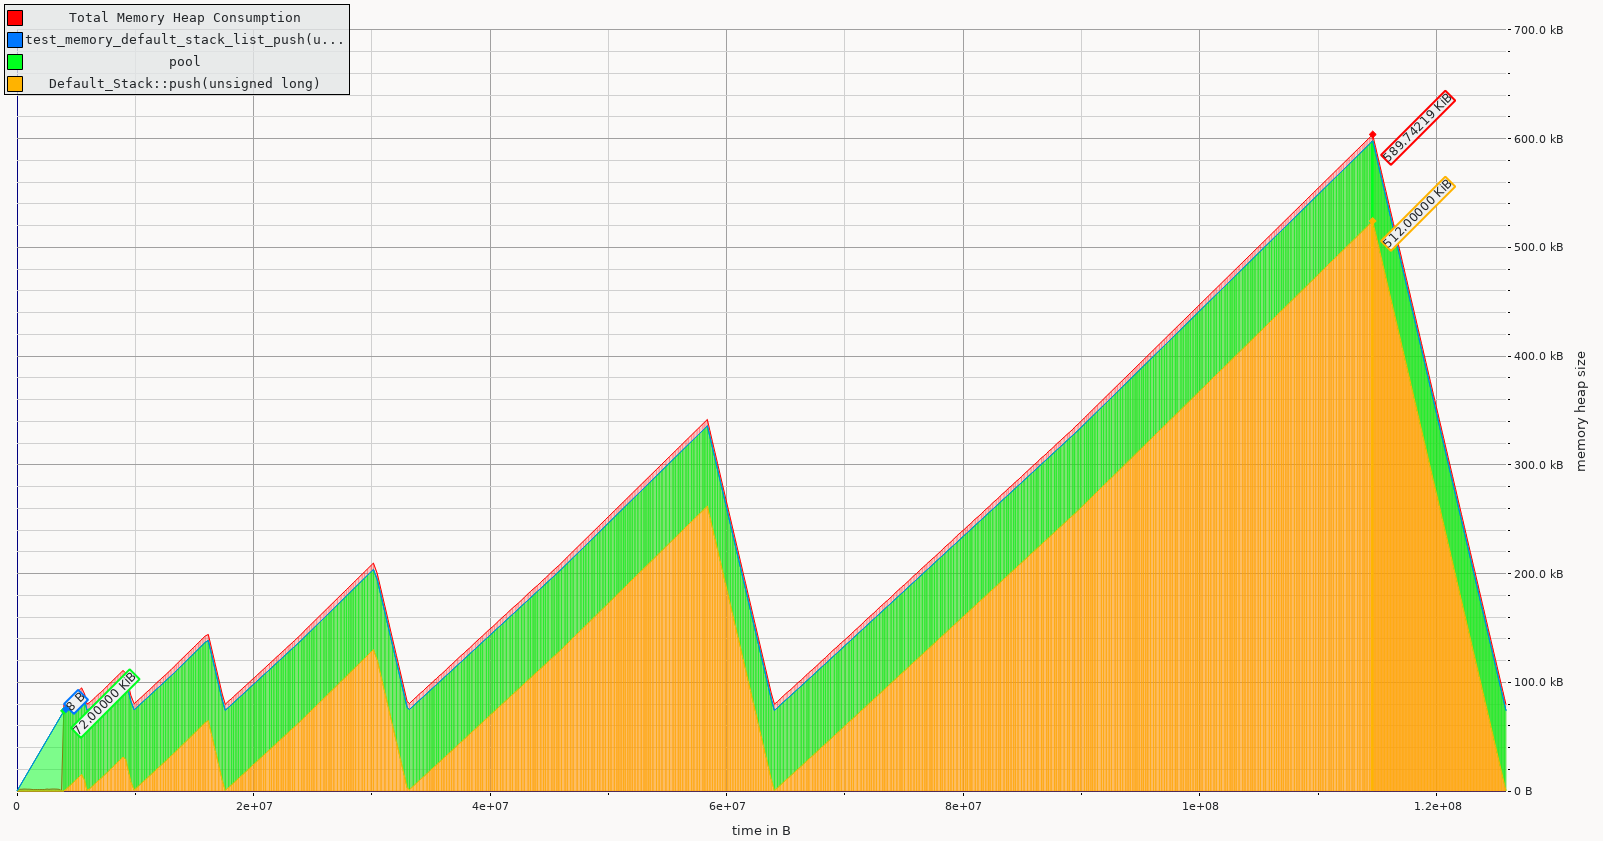
\includegraphics[width=1.0\textwidth]{../../resources/memory_consumption_of_solver_2_benchmark_memory_default_stack.png}
  \caption{}
\end{figure}

Исследуем пик, когда приложение потребляем максимальное количество памяти. Для этого более информативно будет взглянуть на выход \texttt{ms_print}. 
\begin{lstlisting}[caption={}, label={}, style=style_code_block]
-------------------------------------------------------------------------------
  n        time(B)         total(B)   useful-heap(B) extra-heap(B)   stacks(B)
-------------------------------------------------------------------------------
493    114,627,776          866,064          598,024       262,168        5,872
69.05% (598,024B) (heap allocation functions) malloc/new/new[], --alloc-fns, etc.
->60.54% (524,288B) 0x109C1E: Default_Stack::push(unsigned long) (default_stack_list.cpp:13)
| ->59.71% (517,120B) 0x109372: test_memory_default_stack_list_push(unsigned long, unsigned long) (benchmark_memory_default_stack.cpp:43)
| | ->59.71% (517,120B) 0x1094A6: main (benchmark_memory_default_stack.cpp:59)
| |   
| ->00.83% (7,168B) 0x109423: test_memory_default_stack_list_push(unsigned long, unsigned long) (benchmark_memory_default_stack.cpp:51)
|   ->00.83% (7,168B) 0x1094A6: main (benchmark_memory_default_stack.cpp:59)
|     
->08.51% (73,728B) 0x491D03F: pool (eh_alloc.cc:235)
| ->08.51% (73,728B) 0x491D03F: __static_initialization_and_destruction_0 (eh_alloc.cc:373)
|   ->08.51% (73,728B) 0x491D03F: _GLOBAL__sub_I_eh_alloc.cc (eh_alloc.cc:456)
|     ->08.51% (73,728B) 0x40045B6: call_init (dl-init.c:74)
|       ->08.51% (73,728B) 0x40045B6: call_init (dl-init.c:26)
|         ->08.51% (73,728B) 0x40046AC: _dl_init (dl-init.c:121)
|           ->08.51% (73,728B) 0x401CE5F: ??? (in /usr/lib/ld-linux-x86-64.so.2)
|             
->00.00% (8B) 0x1092E7: test_memory_default_stack_list_push(unsigned long, unsigned long) (benchmark_memory_default_stack.cpp:35)
  ->00.00% (8B) 0x1094A6: main (benchmark_memory_default_stack.cpp:59)
\end{lstlisting}

Здесь нас интересуют два фрагмента 
\begin{lstlisting}[caption={}, label={}, style=style_code_block]
  ->60.54\% (524,288B) 0x109C1E: Default_Stack::push(unsigned long) 
  (default_stack_list.cpp:13)
\end{lstlisting}
и
\begin{lstlisting}[caption={}, label={}, style=style_code_block]
  ->00.00\% (8B) 0x1092E7: test_memory_default_stack_list_push(unsigned long, unsigned long) (benchmark_memory_default_stack.cpp:35)
\end{lstlisting}

Первый -- это наши вызовы \texttt{push}, в которых использовались \texttt{new}. Подсказки \texttt{default_stack_list.cpp:13} об этом чётко свидетельствуют. А последние \(8\) байт -- это выделение памяти под сам указатель \texttt{Default_Stack *stack}.

\begin{mdframed}[style=mdfStyleCode]%
  \begin{remark}\rm%
  Выделение памяти \texttt{->08.51\% (73,728B) 0x491D03F:} \texttt{ pool (eh_alloc.cc:235)} не касается нашей темы. Более подробную информацию об этом можно найти в сети.
\end{remark}
\end{mdframed}

Таким образом, согласно выводу \texttt{massif} на нашу структуру при \(n = 2^{15}\) мы тратим \(524288 + 8 = 524296\) байт, а это в точности \(2^{15} \cdot 16 + 8\).

\subsubsection{Подсчёт используемой памяти \texttt{Stack}}

Давайте аналогичным образом, проведём подсчёт для нашей реализации \texttt{Stack} (\texttt{solver_2/solution.hpp}). Так как 
\begin{minted}[breaklines=true]{cpp}
class Stack {
private:
  elem_t B = 0;
  elem_t M = 0;
  Node **stacks; // B + 1 будующих стеков
  elem_t max_value = 0;
  elem_t block_id = 0;
\end{minted}
то на \texttt{Stack *stack = new Stack(B);} мы должны затратить \(5\cdot 8 = 40\) байт. При конструирование в \texttt{stacks} мы положим ещё \(B + 1\) указателей, то есть \(\l(B + 1\r)\cdot 8\) байт. Мы сейчас ведём расчёты, когда у нас тип элементов -- \texttt{size_t}, то есть \texttt{B = 64}. 
Таким образом, на создание \texttt{stack} мы затратим:
\begin{dmath*}
  S_1 = 40 + (64+1)\cdot 8 = 560\text{ байт}
\end{dmath*} 
Теперь взглянем на наш \texttt{push}:
\begin{minted}[breaklines=true]{cpp}
void Stack::push(elem_t value) {
  if (value <= max_value) {
    // В данном случае ни max_value, ни block_id не изменятся.
    stacks[block_id] = new Node(value, stacks[block_id]);
  } else {
    // value > max_value, поэтому потребуется обновление max_value и возможно
    // block_id.
    elem_t new_max_value = value;
    elem_t new_block_id = calculate_block_id(new_max_value);
    if (new_block_id == block_id) {
      // Выполняем стандартное добавление (по формуле 2*value - max_value),
      // поскольку гарантировано не будет переполнения.
      stacks[block_id] =
          new Node(((value - max_value) + value), stacks[block_id]);
    } else {
      // Мы добавляем элемент из другого блока сохраняем старый max, как первый
      // элемент нового блока, чтобы при pop востановить его.
      stacks[new_block_id] = new Node(max_value, stacks[new_block_id]);
    }
    // Перезаписываем max_value и block_id
    max_value = new_max_value;
    block_id = new_block_id;
  }
}
\end{minted}
Очевидно, что в случай \texttt{value > max_value} мы можем попасть конечное число раз зависящее только от количества уникальных элементов в типе \texttt{elem_t}. Худший случай, это когда мы добавляем элементы в стек по возростанию, то есть сперва \(0\), затем \(1\), \(2\) и так далее. В случай \texttt{new_block_id != block_id}, то есть когда мы кладём элемент в новый блок, мы можем попасть максимум \(64\) раза, то есть ровно \(B\) раз.
Но в какой бы случай мы не попали за один вызов \texttt{push} мы гарантировано создадим лишь одну \texttt{Node} (\texttt{Node} у нас аналогичные, как и при рассмотрение \texttt{Default_Stack}, то есть по \(16\) байт).

Таким образом, для добавления \(n\) элементов нам потребуется: \(n\cdot 16 + 560\), то есть при \(n = 2^{15}\) мы должны потратить \(524848\) байт.

Давайте аналогичным образом вызовем \texttt{massif} (см. \texttt{./run_valgrind}) и посмотрим на результаты при \(n = 2^{15}\), что мы получим от \texttt{ms_print} и \texttt{massif-visualizer}:
\begin{figure}[H]
  \centering
  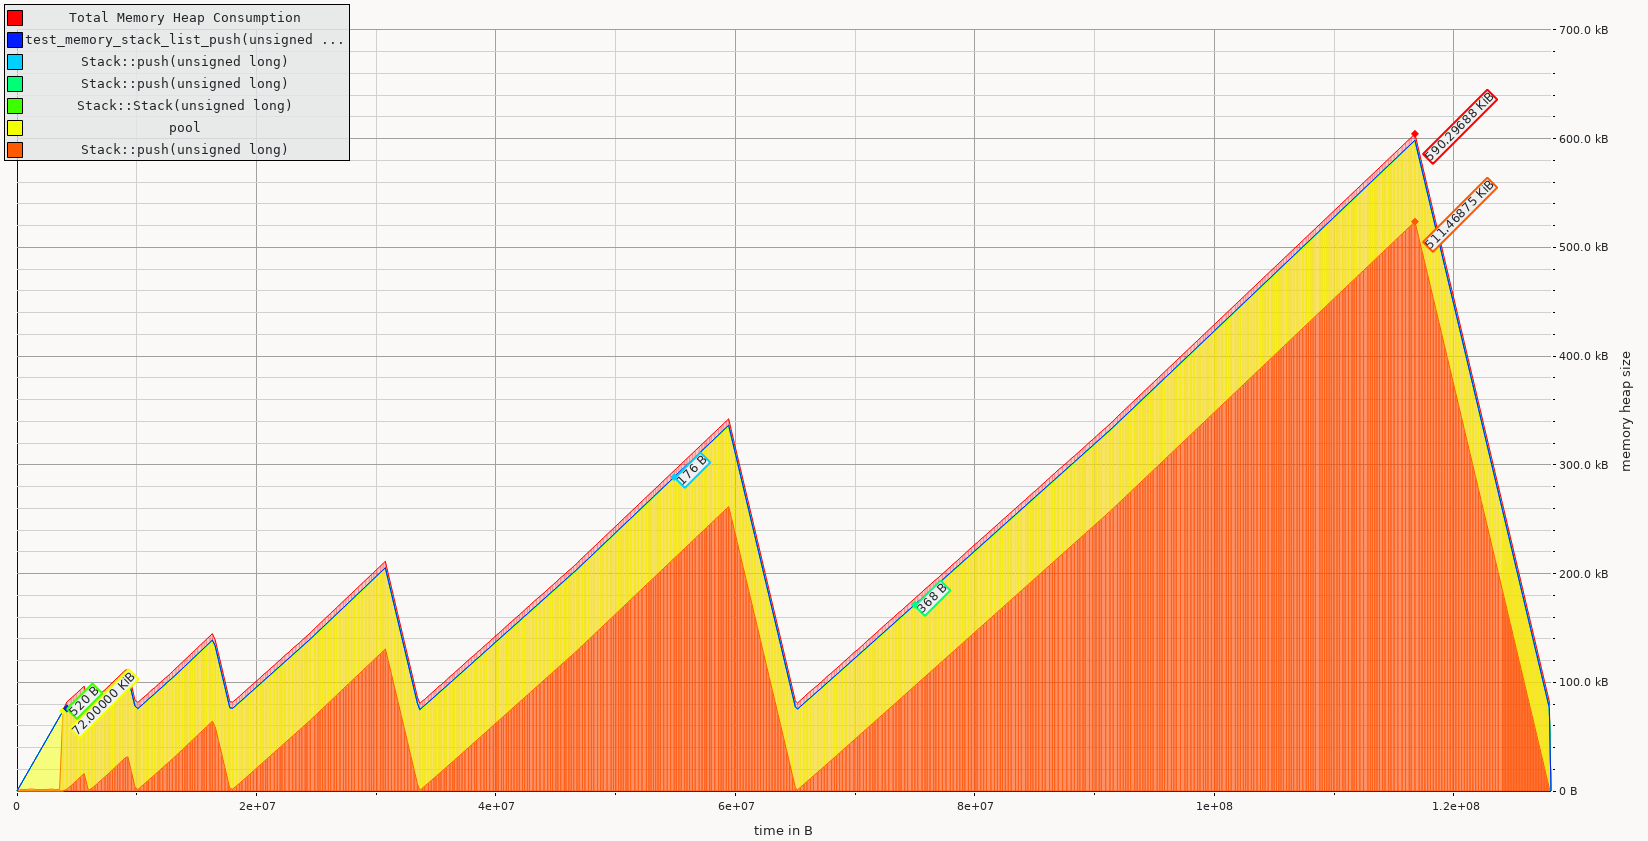
\includegraphics[width=1.0\textwidth]{../../resources/memory_consumption_of_solver_2_benchmark_memory_stack.png}
  \caption{}
\end{figure}
\begin{lstlisting}[caption={}, label={}, style=style_code_block]
-------------------------------------------------------------------------------
  n        time(B)         total(B)   useful-heap(B) extra-heap(B)   stacks(B)
-------------------------------------------------------------------------------
469    116,753,384          866,648          598,576       262,184        5,888
69.07% (598,576B) (heap allocation functions) malloc/new/new[], --alloc-fns, etc.
->60.43% (523,744B) 0x109ED2: Stack::push(unsigned long) (solution.cpp:54)
| ->59.61% (516,576B) 0x1093C6: test_memory_stack_list_push(unsigned long, unsigned long) (benchmark_memory_stack.cpp:43)
| | ->59.61% (516,576B) 0x109537: main (benchmark_memory_stack.cpp:59)
| |   
| ->00.83% (7,168B) 0x109477: test_memory_stack_list_push(unsigned long, unsigned long) (benchmark_memory_stack.cpp:51)
|   ->00.83% (7,168B) 0x109537: main (benchmark_memory_stack.cpp:59)
|     
->08.51% (73,728B) 0x491D03F: pool (eh_alloc.cc:235)
| ->08.51% (73,728B) 0x491D03F: __static_initialization_and_destruction_0 (eh_alloc.cc:373)
|   ->08.51% (73,728B) 0x491D03F: _GLOBAL__sub_I_eh_alloc.cc (eh_alloc.cc:456)
|     ->08.51% (73,728B) 0x40045B6: call_init (dl-init.c:74)
|       ->08.51% (73,728B) 0x40045B6: call_init (dl-init.c:26)
|         ->08.51% (73,728B) 0x40046AC: _dl_init (dl-init.c:121)
|           ->08.51% (73,728B) 0x401CE5F: ??? (in /usr/lib/ld-linux-x86-64.so.2)
|             
->00.06% (520B) 0x109CAB: Stack::Stack(unsigned long) (solution.cpp:13)
| ->00.06% (520B) 0x109346: test_memory_stack_list_push(unsigned long, unsigned long) (benchmark_memory_stack.cpp:35)
|   ->00.06% (520B) 0x109537: main (benchmark_memory_stack.cpp:59)
|     
->00.04% (368B) 0x109F54: Stack::push(unsigned long) (solution.cpp:64)
| ->00.04% (368B) 0x1093C6: test_memory_stack_list_push(unsigned long, unsigned long) (benchmark_memory_stack.cpp:43)
|   ->00.04% (368B) 0x109537: main (benchmark_memory_stack.cpp:59)
|     
->00.02% (176B) 0x109FBB: Stack::push(unsigned long) (solution.cpp:68)
| ->00.02% (176B) 0x1093C6: test_memory_stack_list_push(unsigned long, unsigned long) (benchmark_memory_stack.cpp:43)
|   ->00.02% (176B) 0x109537: main (benchmark_memory_stack.cpp:59)
|     
->00.00% (40B) 0x10932B: test_memory_stack_list_push(unsigned long, unsigned long) (benchmark_memory_stack.cpp:35)
  ->00.00% (40B) 0x109537: main (benchmark_memory_stack.cpp:59)
\end{lstlisting}
Из 
\begin{lstlisting}[caption={}, label={}, style=style_code_block]
->60.43% (523,744B) 0x109ED2: Stack::push(unsigned long) (solution.cpp:54)
\end{lstlisting}
Мы видим, что в основом при вызове \texttt{push} мы попадали в случай \texttt{value <= max_value}. При этом незначительное раз попадали в ситуацию, когда надо было обновить максимум в текущем блоке
\begin{lstlisting}[caption={}, label={}, style=style_code_block]
->00.04% (368B) 0x109F54: Stack::push(unsigned long) (solution.cpp:64)
\end{lstlisting}
Это ожидаемо, поскольку сейчас у нас тип \texttt{size_t} и блоки довольно большие. А число \(n\) очень мало относительно размеров типа \texttt{size_t}.

При этом как мы видим из 
\begin{lstlisting}[caption={}, label={}, style=style_code_block]
->00.02% (176B) 0x109FBB: Stack::push(unsigned long) (solution.cpp:68)
\end{lstlisting}
Мы всего \(176/16 = 11\) раз переходили из одного блока в другой. 

Очевидно, что взависимости от генерации случайных чисел мы будем получать различные соотношения между тремя этими случаями. Однако давайте подсчитаем сколько всего мы затратили памяти. На \texttt{push}:
\begin{dmath*}
  S_2 = 523744 + 368 + 176 = 524288
\end{dmath*}
Плюс у нас ещё есть
\begin{lstlisting}[caption={}, label={}, style=style_code_block]
->00.06% (520B) 0x109CAB: Stack::Stack(unsigned long) (solution.cpp:13)
| ->00.06% (520B) 0x109346: test_memory_stack_list_push(unsigned long, unsigned long) (benchmark_memory_stack.cpp:35)
|   ->00.06% (520B) 0x109537: main (benchmark_memory_stack.cpp:59)

->00.00% (40B) 0x10932B: test_memory_stack_list_push(unsigned long, unsigned long) (benchmark_memory_stack.cpp:35)
  ->00.00% (40B) 0x109537: main (benchmark_memory_stack.cpp:59)
\end{lstlisting}
Первое -- это как раз конструктор \texttt{Stack}, а \texttt{benchmark_memory_stack.cpp:35} -- это создание \texttt{Stack *stack = new Stack(B);}. 

Таким образом, на всю структуру мы затратим:
\begin{dmath*}
  S = 524288 + 560 = 524848 = 2^{15} \cdot 16 + 560
\end{dmath*}


\section{Уточнение задачи}
Рассмотрев два приведённых решения выше, мы можем заметить основную деталь благодоря, которой у нас получилось построить самое решение -- это умение отвечать на вопрос "Пуст ли стек?". 

В первом решение мы отвечали на этот вопрос при помощи счётчика:
\begin{minted}[breaklines=true]{cpp}
// ./solver_1/solution.cpp/pop()
  if (count_elements[block_id] == 0) {
    ...
\end{minted}
Во-втором варианте при помощи проверки, что \texttt{Node *previous_node} не является \texttt{nullptr}.
\begin{minted}[breaklines=true]{cpp}
// ./solver_2/solution.cpp/pop()
  if (previous_node == nullptr) { 
  ...
\end{minted}

И здесь мы возвращаемся к формулировке задачи и вопросу имеет ли стандартный стек, с которым мы выполняем сравнение способ ответа на вопрос "Пуст ли стек?", то есть имеет ли он метод \texttt{empty} (\texttt{is_empty} и другие аналогичные названия)? 
Этот вопрос, с одной стороны, имеет очевидный ответ <<да>>, а, с другой стороны, он не столь очевиден. В отличие от \texttt{push} и \texttt{pop} при рассказе о стеке не так много уделяется внимания вопросу о проверке пустоты стека. Зачастую ответ на него даётся косвенно. Чтобы не быть голословным, давайте рассмотрим ряд источников, причём не будем ограничиваться современными, а окунёмся в историю. 

Насколько мне удалось установить первым упоминанием об стеке является отчёт Алана Тьюринга от 1946 года "A.M. Turing's ACE report of 1946". Его копию не в самом лучшем качестве мне удалось найти на сайте университета Фурмана. Вы можете ознакомиться с ним здесь \href{https://cs.furman.edu/~tallen/csc475/materials/Turing_Report_on_ACE.pdf}{\textcolor{UrlColorText}{\texttt{Turing_Report_on_ACE.pdf}}}. Однако в более хорошем качестве с ним можно ознакомиться в книге \href{https://archive.org/details/amturingsacerepo00turi/page/n3/mode/2up}{\textcolor{UrlColorText}{\texttt{A.M. Turing's ACE report of 1946 and other papers (ISBN-13 978-0262031141) The MIT Press April 3, 1986}}}, которую можно найти на \href{https://archive.org/details/amturingsacerepo00turi/page/n3/mode/2up}{\textcolor{UrlColorText}{archive.org}}. 

Краткое содержание про интересующую нас информацию привёл dave в своём ответе на \href{https://retrocomputing.stackexchange.com/questions/25850/what-motivated-stack-being-invented-originally}{\textcolor{UrlColorText}{stackexchange.com}} (Ниже приведена часть ответа)
\begin{quotation}
  Alan Turing, in his 1946 Report on the ACE described the need for a means to save the return addresses of all active subroutine calls, and to return from such calls in the proper sequence. His routines for subroutine entry and exit were named BURY and UNBURY.

  The return addresses are arranged as a stack. In modern terms, we'd say 'push return address and jump to subroutine', and 'pop address and jump to it'. Or, for the PDP-10 programmers, PUSHJ and POPJ :-).

In Turing's report, he describes the routines thus:
\end{quotation}

\textbf{BURY:}\\
The content of TS 1 with 1 added is transferred to the position indicated in TS 31, and 1 is added to the reference in TS 31. We then proceed to carry out the instruction in TS 1.

\textbf{UNBURY:}\\
The minor cycle whose position is given in TS 31 is taken to be position of the next instruction.

In what we might call 'ACE pseudocode' (see slide 28) the routines are
\begin{lstlisting}[caption={}, label={}, style=style_code_block]
BURY:
M[TS31] <- TS1 + 1; TS31 <- TS31 + 1; go to M[TS1]

UNBURY:
go to M[TS31 <- TS31 - 1]
\end{lstlisting}

\begin{quotation}
  The TS are temporary storage registers, M is memory; TS1 holds the address of the most-recently executed 'type B' (jump) instruction. So we have here a block of memory being used as a stack of return addresses, with TS31 as the stack pointer.
\end{quotation}

Аналогичную идею, но уже более подробную и с явным использованием термина \texttt{stack} мы можем найти в работе \href{https://www.semanticscholar.org/paper/Recursive-Programming-Dijkstra/ff5f9f796a8e0f1908423fab7bebd63f3a8e2f76}{\textcolor{UrlColorText}{\texttt{Dijkstra, Edsger W.. “Recursive Programming.” Numerische Mathematik 2 (1960): 312-318.}}}
\begin{quotation}
  The basic concept of the method is the so-called stack. One uses a stack for storing a sequence of information units that increases and decreases at one end only, i.e. when a unit of information that is no longer of interest is removed from the stack, then this is always the most recently added unit still present in the stack. For example, one can construct a stack as follows: a number of successive storage locations are set aside for the stack and also an administrative quantity, the "stack pointer"{}, that always points to the first free place in the stack (i.e. the value of the stack pointer may be defined as the address of the first free location in the stack; if the stack is empty to start off with, the stack pointer is equal to the start address of the portion of the memory reserved for the stack). When an information unit is added to the stack the stack pointer indicates where this unit must be stored and when this has been done, the value of the stack pointer is accordingly increased. To remove one or more information units from the stack the value of the stack" pointer is suitably decreased.
\end{quotation}

При этом подходе проверка пустоты стека осуществляется путём определения на что указывает указатель стека (вершина стека): "Если стек изначально пуст, то указатель стека равен начальному адресу части памяти, отведенной для стека"{}. 

Также нельзя не упоминуть статью \href{https://www.semanticscholar.org/paper/From-the-Stack-Principle-to-ALGOL-Bauer/16e1cb82b8afd61e4209ea773a8c8976db9cdf4e}{\textcolor{UrlColorText}{\texttt{Bauer, Friedrich L.. “From the Stack Principle to ALGOL.” Software Pioneers (2002).}}}, в которой описываются ранние идеи (1950 года) по использованию стеков, начиная с вычисления выражений, и процессы разработки, которые привели к созданию семейства языков ALGOL. В ней начо стека отмечают специальным символом и именно он является тем маркером, который позволяет понять пуст стек или нет. Скриншот из книги  \href{https://link.springer.com/book/10.1007/978-3-642-59412-0}{\textcolor{UrlColorText}{\texttt{ Software Pioneers Contributions to Software Engineering (2002)}}} ("cellar"{} -- это нынешнее название "stack"{}, о чём можно прочитать ранее в этой же статье):
\begin{figure}[H]
  \centering
  \includegraphics[width=1.0\textwidth]{\ImagesDirName/image1.png}
  \caption{}
\end{figure}

Как мы можем видеть, несмотря на то, что явно для проверки пустоты не использовалось какое-то говорящее название, оно является неотъемлемой частью работы стека.

В более современных трудах, например, в знаменитой работе "The Art of Computer Programming" by Donald E. Knuth (1968) (первый том) определение стека следующее:
\begin{quotation}
  A linear list is a set of \(n \geq 0\) nodes \(X[1], X[2], \dots , X[n]\) whose structural properties essentially involve only the linear (one-dimensional) relative positions of the nodes: the facts that, if \(n > 0\), \(X[1]\) is the first node; when \(1 < k < n\), the \(k\)th node \(X[k]\) is preceded by \(X[k - 1]\) and followed by \(X[k + 1];\) and \(X[n]\) is the last node.

The operations we might want to perform on linear lists include, for example the following
\begin{enumerate}
  \item Gain access to the \(k\)th node of the list to examine and/or change the contents of its fields.
  \item Insert a new node just before the \(k\)th node.
  \item Delete the \(k\)th node.
  \item Combine two or more linear lists into a single list.
  \item Make a copy of a linear list.
  \item Determine the number of nodes in a list.
  \item Sort the nodes of the list into ascending order based on certain fields of the nodes.
  \item Search the list for the occurrence of a node with a particular value in some field.
\end{enumerate}
...

Linear lists in which insertions, deletions, and accesses to values occur almost always at the first or the last node are very frequently encountered, and we give them special names:
  
A \textbf{stack} is a linear list for which all insertions and deletions (and usually all accesses) are made at one end of the list.
\end{quotation}
Далее в книге можно найти рассмотрения различных реализаций линейных списков и соответственно стеков, которые сейчас мы часто называем: "стек на динамическом массиве", "стек на списке", "стек фиксированного размера" и так далее. Но очевидно, что для любой из основ мы легко можем ответить на вопрос об пустоте и соответственно, добавить \texttt{empty}.

Во многих современных источниках, например, в небезызвестных книгах "Introduction to Algorithms" by Thomas H. Cormen, Charles E. Leiserson, Ronald L. Rivest и Clifford Stein (2009) и "Advanced Data Structures" by Peter Brass
Cambridge University Press (2008) мы можем уже прямо найти метод \texttt{Stack-Empty}, где в зависимости от того, на чём основан стек (как реализован линейный список), будут различные реализации. Однако вне зависимости от выбора определения время работы проверки стека будет \(O\l(1\r)\).

Таким образом, я считаю, что тема наличия метода \texttt{empty} в интерфейсе, как базового стека, так и в требуемом стеке с дополнительным методом \texttt{max()}, полностью обоснована.
Интерфейс базового стека, относительно которого будет осуществляться построение требуемого стека: 
\begin{minted}[breaklines=true]{cpp}
class Base_Stack {
...
public:
  // Получение верхнего элемента стека без удаления O(1)
  elem_t top() const; 
  // Проверка на пустоту стека O(1)
  bool empty() const; 
  // Добавление элемента в стек
  void push(elem_t value);
  // Удаление элемента из стека
  elem_t pop();
  ...
};
\end{minted}

\textbf{Замечания:}

  Дополнительно ещё можно обсудить сигнатуру \texttt{pop}, так, например, в \texttt{std::stack} метод \texttt{pop} не возвращает элемент с вершины, а лишь удаляет его. Это считается более правильным решение, как с точки зрения проектирования (метод отвечает, только за удаление, а не берёт на себе две обязанности), так и с точки зрения корректной работы с исключениями. К нашей теме это не относится, а более подробную информацию о причинах такого решения можно найти в Exceptional C++ Style 40 New Engineering Puzzles, Programming Problems, and Solutions by Herb Sutter (2004).

  Также, поскольку мы работаем с конкретными стеками для беззнаковых целых чисел, то нет причин использовать \texttt{elem_t\&} и так далее.

  Также мы целенаправлено не указываем сложность для \texttt{Base_Stack:: push} и \texttt{Base_Stack:: pop}, поскольку в решение задачи, при написание \texttt{push} и \texttt{pop} для требуемого стека (с \texttt{max()}) мы будем использовать методы \texttt{Base_Stack::push} и \texttt{Base_Stack:: pop}, а так как по условию задачи требуется \(O\l(1\r)\) по времени относительно базового стека, то не будет разницы от того сколько времени работают \texttt{Base_Stack:: push} и \texttt{Base_Stack:: pop}. (Время для \texttt{Base_Stack:: push} и \texttt{Base_Stack:: pop} очевидным образом зависит от того, что является основой для \texttt{Base_Stack}.)

  Что касается метода \texttt{top}, то он не считается "основным" методом для стека, поскольку при \texttt{elem_t pop();} мы всегда можем заменить его на вызов \texttt{pop} и \texttt{push}. Однако раз его всегда можно реализовать через \texttt{pop} и \texttt{push} (на практике зачастую это делают более эффективным способом), то нет причин считать, что его не может быть в базовом классе.

\section{Основное решение задачи}

Объявление класса \texttt{Stack}:
\begin{minted}[breaklines=true]{cpp}
class Stack {
private:
  elem_t B = {sizeof(elem_t) * elem_t(8)};
  elem_t M = {~elem_t(0)};

  elem_t max_value = 0; // текущий максимум стека
  // текущий id блока, которому принадлежит max_value
  elem_t block_id = 0;

  Base_Stack *stacks; // B + 1 будующих стеков

  elem_t calculate_block_id(elem_t value);
  bool block_is_empty(elem_t id) const;

public:
  // Конструктор и деструктор
  Stack();
  ~Stack();

  // Проверка на пустоту стека
  bool empty() const;

  elem_t max() const;

  // Добавление элемента в стек
  void push(elem_t value);

  // Удаление элемента из стека
  elem_t pop();

  // Получение верхнего элемента стека без удаления
  elem_t top() const;
};
\end{minted}
\begin{mdframed}[style=mdfStyleCode]%
  \begin{remark}\rm%
  Поля \texttt{B} и \texttt{M}  -- это характеристики типа \texttt{elem_t} и не должны быть членами класса \texttt{Stack}, но для удобства и краткости определим их. Они занимают постоянное место и не зависят от количества элементов, поэтому они никак не повлияют на расчёты. Также при фиксированном \texttt{elem_t} мы могли бы просто создать массив \texttt{stacks}. 
\end{remark}
\end{mdframed}

Перейдём к рассмотрению реализации, которая будет похожа на то, что мы делали при написание \texttt{solver_2}, но с изменениями, чтобы при вызове \texttt{top} не было необходимости смотреть два верхних элементов стека.
\begin{minted}[breaklines=true]{cpp}
Stack::Stack() : stacks(new Base_Stack[B + 1]) {}

Stack::~Stack() { delete[] stacks; }

elem_t log2(elem_t x) {
  [[assume(x != elem_t(0))]];
  return std::bit_width(x) - 1; // bit_width вернёт int
}

elem_t Stack::calculate_block_id(elem_t value) {
  // Вычисляем какому из блоково принадлежит число value:
  if (value == M) {
    // Максимальное число мы обрабатываем отдельно
    return B; // последний из возможных id блока
  } else {
    // Поскольку value < M, то значит M - value != 0, поэтому законно
    // использовать log2 с указанным assume
    return (B - elem_t(1) - log2(M - value));
  }
}

bool Stack::block_is_empty(elem_t id) const { return (stacks[id].empty()); }

bool Stack::empty() const { return ((block_id == 0) && (stacks[0].empty())); }

elem_t Stack::max() const { return max_value; }
\end{minted}
Создание и вычисление \texttt{block_id} без изменения. Мы говорим, что стек пуст, тогда и только тогда, когда \texttt{block_id} равен нулю, и Base_Stack с нулевым идентификатором также пуст.

\begin{minted}[breaklines=true]{cpp}
void Stack::push(elem_t value) {
  if (value <= max_value) {
    // В данном случае ни max_value, ни block_id не изменятся.
    stacks[block_id].push(value); // вызываем Base_Stack::push
  } else {
    // value > max_value, поэтому потребуется обновление max_value и возможно
    // block_id.
    elem_t new_max_value = value;
    elem_t new_block_id = calculate_block_id(new_max_value);
    if (new_block_id == block_id) {
      // Выполняем стандартное добавление (по формуле 2*value - max_value),
      // поскольку гарантировано не будет переполнения.
      // вызываем Base_Stack::push
      stacks[block_id].push(((value - max_value) + value));
    } else {
      // Мы добавляем элемент из другого блока сохраняем старый max, как
      // последний элемент (new_block_id - 1), чтобы при pop востановить его.
      // (new_block_id - 1) >= 0, так как new_block_id >= 1, в данной ветке.
      // вызываем Base_Stack::push
      stacks[new_block_id - elem_t(1)].push(max_value);
    }
    // Перезаписываем max_value и block_id
    max_value = new_max_value;
    block_id = new_block_id;
  }
}
\end{minted}
В \texttt{push} в случае, когда мы добавляем значение \texttt{value} из блока с \texttt{new_block_id} большим, чем текущий \texttt{block_id}, то на вершину блока с id равным \texttt{new_block_id - 1} мы сохраняем текущий максимум. Причём заметим, что после последующих \texttt{push} мы никогда не положим на этот сохранённый максимум ни одного нового значения. Действительно, если впоследствии будут приходить значения меньшие, то они уже будут попадать в блок с \texttt{block_id == new_block}.

\begin{minted}[breaklines=true]{cpp}
elem_t Stack::pop() {
  // Мы знаем текущий max_value, его block_id и верхний элемент стека,
  // кототрый может быть: предыдущим max, истинным добавленным значением,
  // значением, для определения предыдущего max.
  bool block_empty = stacks[block_id].empty();
  if (block_empty && (block_id != 0)) {
    // Блок пустой и block_id != 0, значит текущий max -- это последний элемент,
    // который необходимо вернуть, а в предыдущем блоке на вершине лежит старый
    // max.
    elem_t res = max_value;
    elem_t prev_max =
        stacks[block_id - elem_t(1)].pop(); // Вызываем Base_Stack::pop
    block_id = calculate_block_id(prev_max);
    max_value = prev_max;
    return res;
  }
  // Далее block_empty = false, поскольку если здесь он равен true, то значит
  // block_empty && (block_id == 0) == true, но тогда это означает, что мы
  // пытаемся извлечь из пустого стека. Здесь можно либо выбросить исключение,
  // либо как-то иначе обрабатывать данную ошибку. Мы же просто скажем, что это
  // UB

  // возвращаем не последний элемент из блока
  elem_t element = stacks[block_id].pop(); // Вызываем Base_Stack::pop
  if (element <= max_value) {
    // element -- истинное добавленное значение
    return element;
  } else {
    // element -- значение, которое будет использоваться, для вычисления
    // прошлого max_value, а текущее max_value -- это истинное добавленное
    // значение,
    elem_t res = max_value;
    // востановим прошлый максимум по формуле 2 * max_value - element;
    // Чтобы не было переполнения в промежуточных шагах:
    elem_t diff = element - max_value;
    // последнее корректно, так как в случае element > max_value

    // (max_value - diff =  max_value - (element - max_value) = 2*max_value
    // - element)
    max_value = max_value - diff;
    return res;
  }
}
\end{minted}
Метод \texttt{pop} теперь стал более простым и понятным. Основной принцип его работы описан в комментариях. Отметим лишь то, что при вызове \texttt{pop} мы вызываем один раз \texttt{Base_Stack:: empty} и один раз \texttt{Base_Stack:: pop}. Поскольку временная сложность \texttt{Base_Stack:: empty} равна \(O\l(1\r)\), то временная сложность \texttt{pop} аналогична временной сложности \texttt{Base_Stack:: pop}.

\begin{minted}[breaklines=true]{cpp}
elem_t Stack::top() const {
  bool block_empty = stacks[block_id].empty();
  if (block_empty && (block_id != 0)) {
    // Блок пустой и block_id != 0, значит текущий max -- это последний элемент,
    // который необходимо вернуть
    return max_value;
  }
  // Опять же, если block_empty == true и block_id == 0, то тогда мы пытаемся
  // узнать элемент пустого стека. Это можно обработать в ветви else. Но мы
  // скажем, что это просто UB.
  // Далее block_empty == false
  elem_t element = stacks[block_id].top(); // Вызываем Base_Stack::top

  if (element <= max_value) {
    // element -- истинное добавленное значение
    return element;
  } else {
    // element -- значение, которое будет использоваться, для вычисления
    // прошлого max_value, а текущее max_value -- это истинное добавленное
    // значение,
    return max_value;
  }
}
\end{minted}
Метод \texttt{top} мы изменили так, чтобы не требовалось заглядывать на \(2\) элемента назад. Основной принцип его работы описан в комментариях. Отметим, что при вызове \texttt{top} мы вызываем один раз \texttt{Base_Stack:: empty} и один раз \texttt{Base_Stack:: top}. Поскольку временная сложность \texttt{Base_Stack:: empty} равна \(O\l(1\r)\), то временная сложность \texttt{top} аналогична временной сложности \texttt{Base_Stack:: top}, то есть постоянная.


\subsection{Тестирование и замеры}

Тестирование корректности вычисления \texttt{push}, \texttt{pop}, \texttt{top} и \texttt{max} проведём аналогично, как и для решения \texttt{solver_1}. На тех же входных данных. Более подробно смотреть в \texttt{tests.md}.

Корректность по времени и памяти очевидна из кода. Однако мы всё равно убедимся в этом при помощи практических замеров. Сначало проанализируем потребляемую память. 

Исходя из нашего определения \texttt{Stack}. При создание \texttt{Stack *stack = new Stack();} мы потратим \(S_0\) у.е для хранения самого указателия \texttt{Stack *}, который будет лежать на стеке. Затем уже будет потребляться память в куче: \(4\cdot S_1\) у.е. (условных единиц) на хранение:
\begin{minted}[breaklines=true]{cpp}
  elem_t B = {sizeof(elem_t) * elem_t(8)};
  elem_t M = {~elem_t(0)};
  elem_t max_value = 0; 
  elem_t block_id = 0;
\end{minted}
где \(S_1\) -- сколько условных единиц занимает элемент типа \texttt{elem_t} (Если условные единицы -- это биты, то по определению \(B\), мы имеем\(S_1 = B\)). 
Плюс \(S_2\) у.е. для хранения \texttt{Base_Stack *stacks;}, то есть \(S_2\) -- сколько условных единиц занимает указатель на \texttt{Base_Stack}.

Во время создания объекта в конструкторе мы ещё потратим \((B + 1)\cdot S_3\) у.е., где \(S_3\) -- сколько условных единиц занимает элемент типа \texttt{Base_Stack}. Плюс для корректной работы \texttt{delete[]} будет сохранено число, которое будет сообщать о количестве. Его значение будет равно \(B + 1\), поэтому достаточно будет \(log_2(B + 1)\) бит для его хранения. Однако компилятор выделит под него \texttt{sizeof(size_t)}. Для нас здесь важно, что количество выделенной памяти не зависит от \(n\), а зависит от \(B\). Обозначим количество памяти для хранения этого числа \(S_4\) у.е.

При добавление \(n\) элементов в стек, мы затратим \(n\cdot S_5\) у.е., где \(S_5\) -- сколько условных единиц требуется для хранения одного элемента в \texttt{Base_Stack}. (\(S_5\) не всегда равно \(S_1\), например, если реализация \texttt{Base_Stack} основана на односвязном списке. Единственное, что можно утверждать -- это \(S_1 \leq S_5\))

Таким образом, суммарно для хранения \(n\) элементов в стеке потребуется:
\begin{dmath*}
  S = S_0 + \underbrace{4\cdot S_1 + S_2 + (B + 1)\cdot S_3 + S_4 + n \cdot S_5}_{S_h \text{ -- в куче}}
\end{dmath*}

При этом для создания \texttt{Base_Stack *base_stack = new Base_Stack()} и хранении \(n\) элементов в нём нам потребуется:
\begin{dmath*}
  S' = S_2 + \underbrace{S_3 + n\cdot S_4}_{S'_h \text{ -- в куче}}
\end{dmath*}
Таким образом, разница по памяти составляет:
\begin{dmath*}
  \Delta = S - S' = S_0 + 4\cdot S_1 + B \cdot S_3 + S_4 
\end{dmath*}
Разница в диномической памяти соответсвенно будет 
\begin{dmath*}
  \Delta_h =  4\cdot S_1 + S_2 + B \cdot S_3 + S_4
\end{dmath*}

Таким образом, \(\Delta\) и \(\Delta_{h}\) имеют значения не зависящие от \(n\), то есть получено требуемое \(O\l(1\r)\).

Чтобы потвердить это на практике, давайте зафиксируем тип \texttt{elem_t = size_t} и будем вести расчёты в байтах. Тогда \(S_1 = 8\) байт, \(S_0 = S_2 = S_4 = 8 \) байт (на \(64\)-битной машине размер указателей будет равен \(8\) байт). Таким образом, на выходе замеров мы должны получить разницу в 
\begin{dmath}[labelN={5}]
  \Delta_h = 32 + 8 + 64\cdot S_3 + 8 = 48 +  64\cdot S_3 \text{ байт}
\end{dmath}


\begin{mdframed}[style=mdfStyleCode]%
  \begin{remark}\rm%
  При разных \texttt{elem_t}, могут быть ситуации, когда в \texttt{Stack} потребуется ещё дополнительная память для выравнивания. Однако на это потребуется также некоторое постоянное значение, зависящее только от \texttt{elem_t}.
\end{remark}
\end{mdframed}

\subsection{\texttt{Base_Stack} на \texttt{std::list}}

Первым делом выполним измерения относительно:
\begin{minted}[breaklines=true]{cpp}
#include <stack>

#include <list>
using elem_t = size_t;

class Base_Stack {
private:
  std::stack<elem_t, std::list<elem_t>> stack;

public:
  void push(const elem_t &value) { stack.push(value); }
  bool empty() { return stack.empty(); }

  elem_t pop() {
    elem_t element = stack.top();
    stack.pop();
    return element;
  }

  elem_t top() { return stack.top(); }
};
\end{minted}
\begin{mdframed}[style=mdfStyleCode]%
  \begin{remark}\rm%
  \texttt{std::stack::pop} не возвращает последний элемент. Поэтому \texttt{Base_Stack} это, по сути, обёртка над \texttt{std::stack} с "переопределённым" методом \texttt{pop} и ровно с четырьмя методами.
\end{remark}
\end{mdframed}

(Записываем это в \texttt{./src/base_stack/base_stack.hpp} и собираем \texttt{solver_3}, после чего запускаем \texttt{valgrind} с результатами компиляции \texttt{benchmark_memory_stack.cpp} и \texttt{benchmark_memory}\-\texttt{_base_stack.cpp} для нахождения соответственно \(S_{h}\) и \(S'_{h}\).)

Результаты для \texttt{Stack}:
\begin{figure}[H]
  \centering
  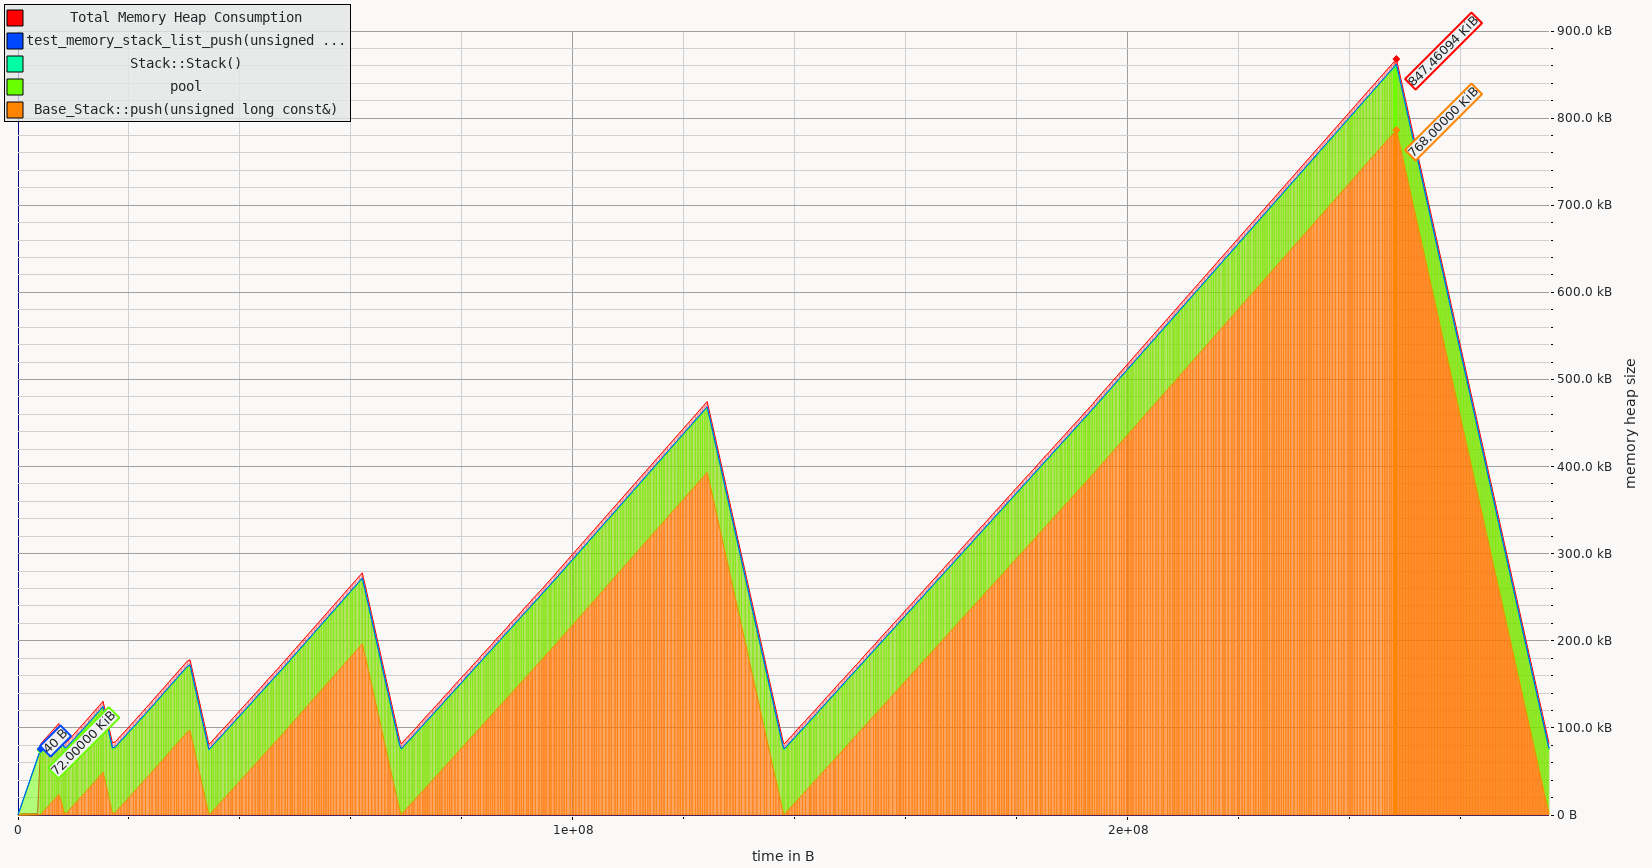
\includegraphics[width=1.0\textwidth]{../../resources/memory_consumption_of_solver3_benchmark_memory_stack_with_list_1.png}
  \caption{\texttt{./results/massif_solver3_benchmark_memory_stack_for_latex.out}}
\end{figure}

Рассмотрим самый большой пик, а именно при \(n = 2^{15}\) (Подробную информацию см. в \texttt{./results/massif_solver3_\-benchmark_memory_stack_\-for_latex.result}):
\begin{lstlisting}[caption={}, label={}, style=style_code_block]
-------------------------------------------------------------------------------
  n        time(B)         total(B)   useful-heap(B) extra-heap(B)   stacks(B)
-------------------------------------------------------------------------------
626    248,444,104        1,392,120          861,768       524,320        6,032
61.90% (861,768B) (heap allocation functions) malloc/new/new[], --alloc-fns, etc.
->56.49% (786,432B) 0x10AC80: std::__new_allocator<std::_List_node<unsigned long> >::allocate(unsigned long, void const*) (new_allocator.h:151)
| ->56.49% (786,432B) 0x10AA8E: allocate (allocator.h:196)
|   ->56.49% (786,432B) 0x10AA8E: allocate (alloc_traits.h:478)
|     ->56.49% (786,432B) 0x10AA8E: std::__cxx11::_List_base<unsigned long, std::allocator<unsigned long> >::_M_get_node() (stl_list.h:518)
|       ->56.49% (786,432B) 0x10A8BF: std::_List_node<unsigned long>* std::__cxx11::list<unsigned long, std::allocator<unsigned long> >::_M_create_node<unsigned long const&>(unsigned long const&) (stl_list.h:710)
|         ->56.49% (786,432B) 0x10A69D: void std::__cxx11::list<unsigned long, std::allocator<unsigned long> >::_M_insert<unsigned long const&>(std::_List_iterator<unsigned long>, unsigned long const&) (stl_list.h:2004)
|           ->56.49% (786,432B) 0x10A473: std::__cxx11::list<unsigned long, std::allocator<unsigned long> >::push_back(unsigned long const&) (stl_list.h:1306)
|             ->56.49% (786,432B) 0x10A334: std::stack<unsigned long, std::__cxx11::list<unsigned long, std::allocator<unsigned long> > >::push(unsigned long const&) (stl_stack.h:259)
|               ->56.49% (786,432B) 0x10A234: Base_Stack::push(unsigned long const&) (base_stack.hpp:11)
|                 ->56.41% (785,256B) 0x109F03: Stack::push(unsigned long) (solution.cpp:33)
|                 | ->55.64% (774,528B) 0x1093FC: test_memory_stack_list_push(unsigned long, unsigned long) (benchmark_memory_stack.cpp:43)
|                 | | ->55.64% (774,528B) 0x10956D: main (benchmark_memory_stack.cpp:59)
|                 | |   
|                 | ->00.77% (10,728B) 0x1094AD: test_memory_stack_list_push(unsigned long, unsigned long) (benchmark_memory_stack.cpp:51)
|                 |   ->00.77% (10,728B) 0x10956D: main (benchmark_memory_stack.cpp:59)
|                 |     
|                 ->00.06% (888B) 0x109F7F: Stack::push(unsigned long) (solution.cpp:43)
|                 | ->00.06% (888B) 0x1093FC: test_memory_stack_list_push(unsigned long, unsigned long) (benchmark_memory_stack.cpp:43)
|                 |   ->00.06% (888B) 0x10956D: main (benchmark_memory_stack.cpp:59)
|                 |     
|                 ->00.02% (288B) 0x109FB4: Stack::push(unsigned long) (solution.cpp:49)
|                   ->00.02% (264B) 0x1093FC: test_memory_stack_list_push(unsigned long, unsigned long) (benchmark_memory_stack.cpp:43)
|                   | ->00.02% (264B) 0x10956D: main (benchmark_memory_stack.cpp:59)
|                   |   
|                   ->00.00% (24B) 0x1094AD: test_memory_stack_list_push(unsigned long, unsigned long) (benchmark_memory_stack.cpp:51)
|                     ->00.00% (24B) 0x10956D: main (benchmark_memory_stack.cpp:59)
|                       
->05.30% (73,728B) 0x491E03F: pool (eh_alloc.cc:235)
| ->05.30% (73,728B) 0x491E03F: __static_initialization_and_destruction_0 (eh_alloc.cc:373)
|   ->05.30% (73,728B) 0x491E03F: _GLOBAL__sub_I_eh_alloc.cc (eh_alloc.cc:456)
|     ->05.30% (73,728B) 0x40045B6: call_init (dl-init.c:74)
|       ->05.30% (73,728B) 0x40045B6: call_init (dl-init.c:26)
|         ->05.30% (73,728B) 0x40046AC: _dl_init (dl-init.c:121)
|           ->05.30% (73,728B) 0x401CE5F: ??? (in /usr/lib/ld-linux-x86-64.so.2)
|             
->00.11% (1,568B) 0x109CC5: Stack::Stack() (solution.cpp:4)
| ->00.11% (1,568B) 0x10937C: test_memory_stack_list_push(unsigned long, unsigned long) (benchmark_memory_stack.cpp:35)
|   ->00.11% (1,568B) 0x10956D: main (benchmark_memory_stack.cpp:59)
|     
->00.00% (40B) 0x10936B: test_memory_stack_list_push(unsigned long, unsigned long) (benchmark_memory_stack.cpp:35)
  ->00.00% (40B) 0x10956D: main (benchmark_memory_stack.cpp:59)
\end{lstlisting}

Нас интересует в первую очередь
\begin{lstlisting}[caption={}, label={}, style=style_code_block]
->56.49% (786,432B) 0x10A234: Base_Stack::push(unsigned long const&) (base_stack.hpp:11)
  ->56.41% (785,256B) 0x109F03: Stack::push(unsigned long) (solution.cpp:33)
  | ->55.64% (774,528B) 0x1093FC: test_memory_stack_list_push(unsigned long, unsigned long) (benchmark_memory_stack.cpp:43)
  | | ->55.64% (774,528B) 0x10956D: main (benchmark_memory_stack.cpp:59)
  | |   
  | ->00.77% (10,728B) 0x1094AD: test_memory_stack_list_push(unsigned long, unsigned long) (benchmark_memory_stack.cpp:51)
  |   ->00.77% (10,728B) 0x10956D: main (benchmark_memory_stack.cpp:59)
  |     
  ->00.06% (888B) 0x109F7F: Stack::push(unsigned long) (solution.cpp:43)
  | ->00.06% (888B) 0x1093FC: test_memory_stack_list_push(unsigned long, unsigned long) (benchmark_memory_stack.cpp:43)
  |   ->00.06% (888B) 0x10956D: main (benchmark_memory_stack.cpp:59)
  |     
  ->00.02% (288B) 0x109FB4: Stack::push(unsigned long) (solution.cpp:49)
    ->00.02% (264B) 0x1093FC: test_memory_stack_list_push(unsigned long, unsigned long) (benchmark_memory_stack.cpp:43)
    | ->00.02% (264B) 0x10956D: main (benchmark_memory_stack.cpp:59)
    |   
    ->00.00% (24B) 0x1094AD: test_memory_stack_list_push(unsigned long, unsigned long) (benchmark_memory_stack.cpp:51)
      ->00.00% (24B) 0x10956D: main (benchmark_memory_stack.cpp:59)
\end{lstlisting}
Здесь мы видим, что всего при помощи \texttt{push} мы выделили \(786432\) байта. (Это слагаемое \(n\cdot S_5\)).

А в конструкторе и при создание объекта \(Stack* stack\) мы потратили
\begin{lstlisting}[caption={}, label={}, style=style_code_block]
->00.11% (1,568B) 0x109CC5: Stack::Stack() (solution.cpp:4)
| ->00.11% (1,568B) 0x10937C: test_memory_stack_list_push(unsigned long, unsigned long) (benchmark_memory_stack.cpp:35)
|   ->00.11% (1,568B) 0x10956D: main (benchmark_memory_stack.cpp:59)
|     
->00.00% (40B) 0x10936B: test_memory_stack_list_push(unsigned long, unsigned long) (benchmark_memory_stack.cpp:35)
  ->00.00% (40B) 0x10956D: main (benchmark_memory_stack.cpp:59)
\end{lstlisting}
Первое это \((B + 1)\cdot S_3 + S_4\), а второе это \(4\cdot S_1 + S_2\).

Таким образом, 
\begin{dmath*}
  S_h = 786432 + 1568 + 40 = 788040
\end{dmath*}

Аналогично посмотрим для \texttt{Base_Stack} (\texttt{./src/solver_3/benchmarks/\-benchmark\-_memory_\-base_stack.cpp}).
\begin{figure}[H]
  \centering
  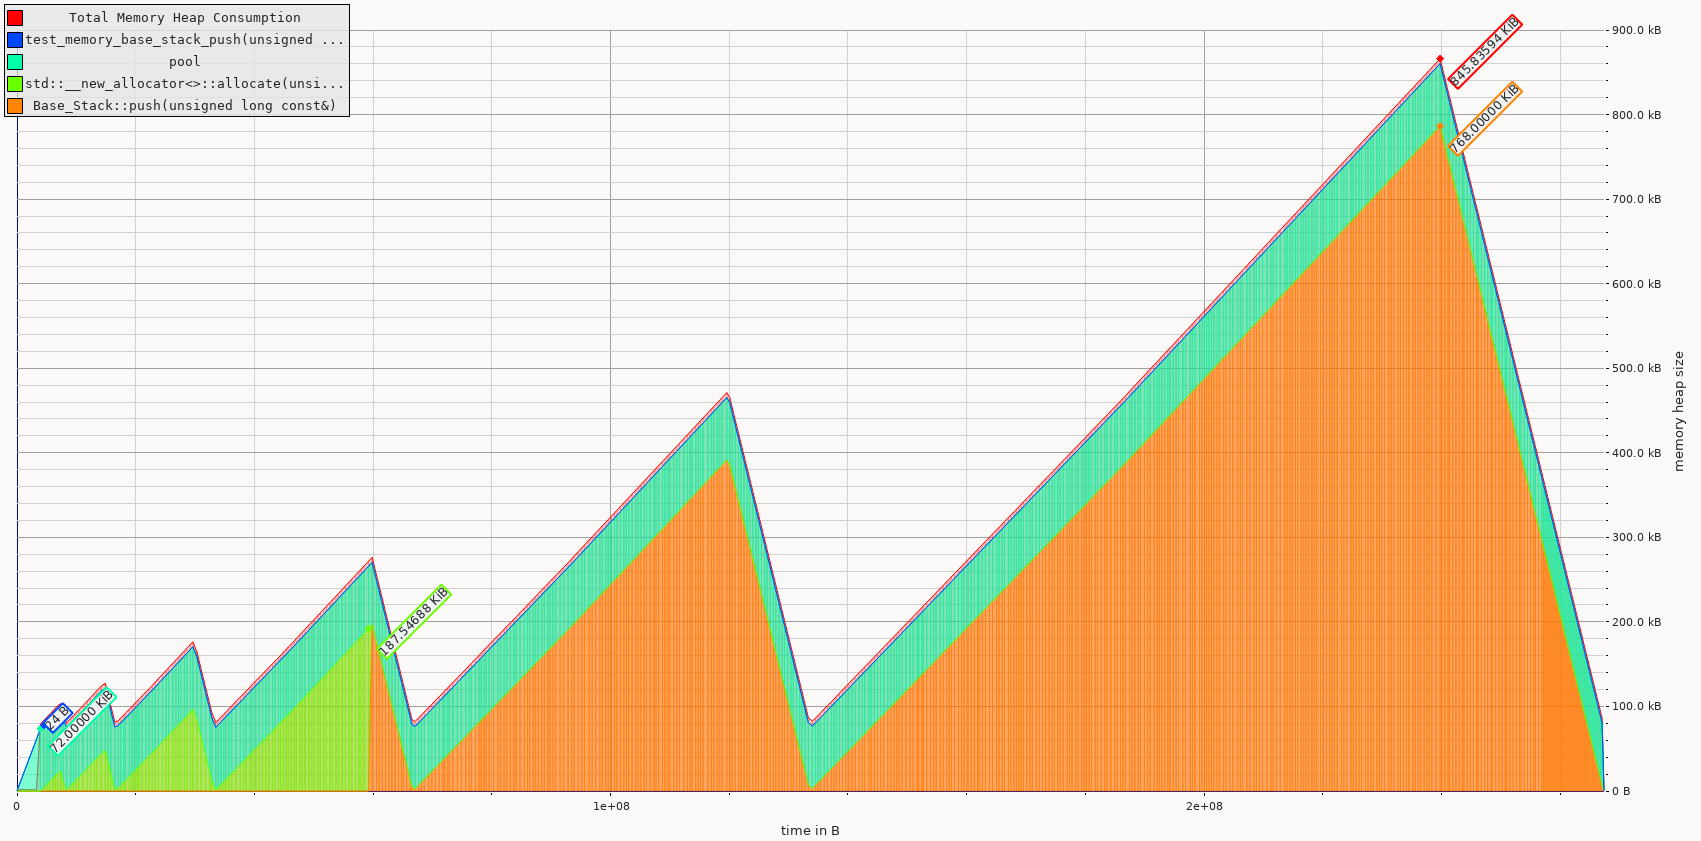
\includegraphics[width=1.0\textwidth]{../../resources/memory_consumption_of_solver3_benchmark_memory_base_stack_with_list_1.png}
  \caption{\texttt{./results/massif_solver3_benchmark_memory_base_stack_for_latex.out}}
\end{figure}

Рассмотрим более подробно пик при \(n = 2^{15}\)
\begin{lstlisting}[caption={}, label={}, style=style_code_block]
-------------------------------------------------------------------------------
  n        time(B)         total(B)   useful-heap(B) extra-heap(B)   stacks(B)
-------------------------------------------------------------------------------
462    239,776,880        1,390,448          860,184       524,312        5,952
61.86% (860,184B) (heap allocation functions) malloc/new/new[], --alloc-fns, etc.
->56.56% (786,432B) 0x10A3F0: std::__new_allocator<std::_List_node<unsigned long> >::allocate(unsigned long, void const*) (new_allocator.h:151)
| ->56.56% (786,432B) 0x10A1FE: allocate (allocator.h:196)
|   ->56.56% (786,432B) 0x10A1FE: allocate (alloc_traits.h:478)
|     ->56.56% (786,432B) 0x10A1FE: std::__cxx11::_List_base<unsigned long, std::allocator<unsigned long> >::_M_get_node() (stl_list.h:518)
|       ->56.56% (786,432B) 0x109E3B: std::_List_node<unsigned long>* std::__cxx11::list<unsigned long, std::allocator<unsigned long> >::_M_create_node<unsigned long const&>(unsigned long const&) (stl_list.h:710)
|         ->56.56% (786,432B) 0x109BBB: void std::__cxx11::list<unsigned long, std::allocator<unsigned long> >::_M_insert<unsigned long const&>(std::_List_iterator<unsigned long>, unsigned long const&) (stl_list.h:2004)
|           ->56.56% (786,432B) 0x10981D: std::__cxx11::list<unsigned long, std::allocator<unsigned long> >::push_back(unsigned long const&) (stl_list.h:1306)
|             ->56.56% (786,432B) 0x1096CA: std::stack<unsigned long, std::__cxx11::list<unsigned long, std::allocator<unsigned long> > >::push(unsigned long const&) (stl_stack.h:259)
|               ->56.56% (786,432B) 0x109610: Base_Stack::push(unsigned long const&) (base_stack.hpp:11)
|                 ->55.79% (775,680B) 0x1093FC: test_memory_base_stack_push(unsigned long, unsigned long) (benchmark_memory_base_stack.cpp:43)
|                 | ->55.79% (775,680B) 0x10953E: main (benchmark_memory_base_stack.cpp:59)
|                 |   
|                 ->00.77% (10,752B) 0x1094BB: test_memory_base_stack_push(unsigned long, unsigned long) (benchmark_memory_base_stack.cpp:51)
|                   ->00.77% (10,752B) 0x10953E: main (benchmark_memory_base_stack.cpp:59)
|                     
->05.30% (73,728B) 0x491E03F: pool (eh_alloc.cc:235)
| ->05.30% (73,728B) 0x491E03F: __static_initialization_and_destruction_0 (eh_alloc.cc:373)
|   ->05.30% (73,728B) 0x491E03F: _GLOBAL__sub_I_eh_alloc.cc (eh_alloc.cc:456)
|     ->05.30% (73,728B) 0x40045B6: call_init (dl-init.c:74)
|       ->05.30% (73,728B) 0x40045B6: call_init (dl-init.c:26)
|         ->05.30% (73,728B) 0x40046AC: _dl_init (dl-init.c:121)
|           ->05.30% (73,728B) 0x401CE5F: ??? (in /usr/lib/ld-linux-x86-64.so.2)
|             
->00.00% (24B) 0x109357: test_memory_base_stack_push(unsigned long, unsigned long) (benchmark_memory_base_stack.cpp:35)
  ->00.00% (24B) 0x10953E: main (benchmark_memory_base_stack.cpp:59)
\end{lstlisting}
Нас в первую очередь интересует:
\begin{lstlisting}[caption={}, label={}, style=style_code_block]
->56.56% (786,432B) 0x109610: Base_Stack::push(unsigned long const&) (base_stack.hpp:11)
  ->55.79% (775,680B) 0x1093FC: test_memory_base_stack_push(unsigned long, unsigned long) (benchmark_memory_base_stack.cpp:43)
  | ->55.79% (775,680B) 0x10953E: main (benchmark_memory_base_stack.cpp:59)
  |   
  ->00.77% (10,752B) 0x1094BB: test_memory_base_stack_push(unsigned long, unsigned long) (benchmark_memory_base_stack.cpp:51)
    ->00.77% (10,752B) 0x10953E: main (benchmark_memory_base_stack.cpp:59)
\end{lstlisting}      
Мы видим, что на \texttt{push} было потрачено \texttt{786432} байт, то есть для добавления одного элемента требуется \(S_5 = 786432/2^{15} = 24\) байта. (Действительно, поскольку \texttt{std::list} -- это двусвязный список и его нода имеет два указателя и элемент данных). 

Пустой же \texttt{Base_Stack} после инициализации занимает 
\begin{lstlisting}[caption={}, label={}, style=style_code_block]
->00.00% (24B) 0x109357: test_memory_base_stack_push(unsigned long, unsigned long) (benchmark_memory_base_stack.cpp:35)
  ->00.00% (24B) 0x10953E: main (benchmark_memory_base_stack.cpp:59)
\end{lstlisting}
ровно \(24\) байта, то есть в наших обозначениях \(S_3 = 24\).

Таким образом, 
\begin{dmath*}
  S'_h = 786432 + 24 = 786456 
\end{dmath*}
тогда
\begin{dmath*}
  \Delta_h = S_h - S'_h = 788040 - 786456 = 1584 
\end{dmath*}
или по формуле (\dref{5}): \(48 + 64*24 = 1584\).


Аналогичным образом, можно подсчитать \(\Delta_{h}\) для других пиков. Однако для этого уже следует изменить тест. В идеале вообще пересобирать тест лишь для одного конкретного \(n\), поскольку \texttt{massif} может максимум сделать \(1000\) снимков. Поэтому, если он точно определяет момент, когда мы выделяем \(2^15\) (абсолютный пик всего теста), то вот для \(2^{10}\) он уже не может сделать точный снимок. Ближайший к этому пику -- это снимок с номером \(15\). Однако в нём мы всего выделяем \(23640\) байт, что меньше чем \(2^{10} \cdot 24\). Аналогичная проблема и для \texttt{Base_Stack}, для которого нет снимка в при \(n = 2^{15}\).

Так давайте проведём замеры для \(n = 2^{20}\). 
\begin{figure}[H]
  \centering
  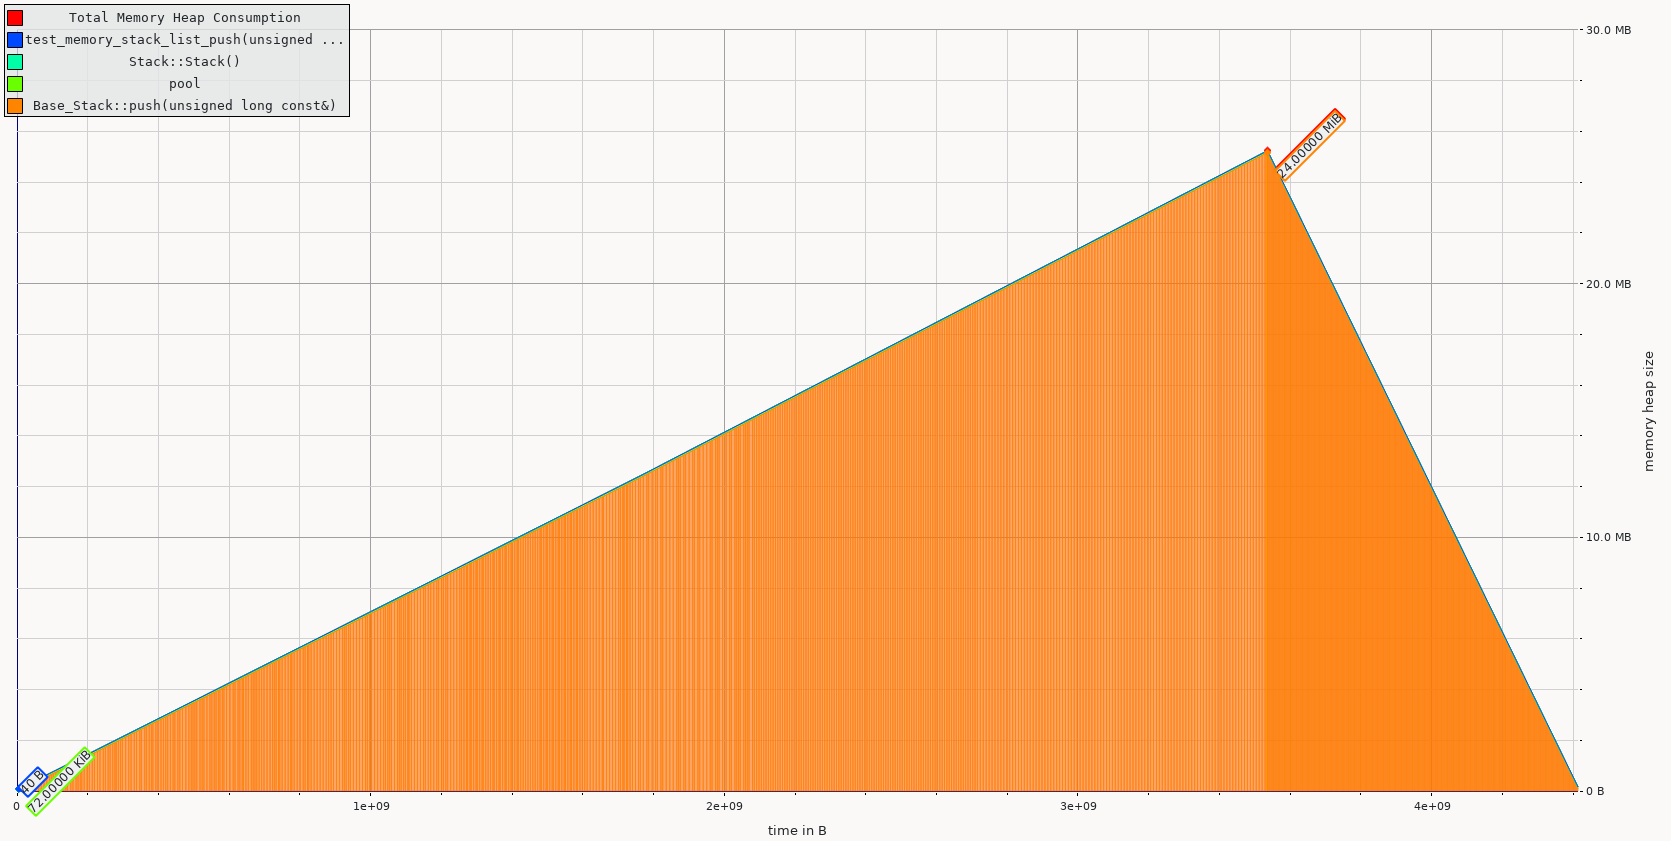
\includegraphics[width=1.0\textwidth]{../../resources/memory_consumption_of_solver3_benchmark_memory_stack_with_list_2.png}
  \caption{\texttt{./results/massif_solver3_benchmark_memory_stack_for_latex_2.out}}
\end{figure}
Для \texttt{Stack} рассмотрим подробно его пик:
\begin{lstlisting}[caption={}, label={}, style=style_code_block]
->59.88% (25,165,824B) 0x10A234: Base_Stack::push(unsigned long const&) (base_stack.hpp:11)
  ->59.88% (25,163,640B) 0x109F03: Stack::push(unsigned long) (solution.cpp:33)
  | ->58.96% (24,776,568B) 0x1093FC: test_memory_stack_list_push(unsigned long, unsigned long) (benchmark_memory_stack.cpp:43)
  | | ->58.96% (24,776,568B) 0x10956D: main (benchmark_memory_stack.cpp:59)
  | |   
  | ->00.92% (387,072B) 0x1094AD: test_memory_stack_list_push(unsigned long, unsigned long) (benchmark_memory_stack.cpp:51)
  |   ->00.92% (387,072B) 0x10956D: main (benchmark_memory_stack.cpp:59)
  |     
  ->00.00% (1,776B) 0x109F7F: Stack::push(unsigned long) (solution.cpp:43)
  | ->00.00% (1,776B) 0x1093FC: test_memory_stack_list_push(unsigned long, unsigned long) (benchmark_memory_stack.cpp:43)
  |   ->00.00% (1,776B) 0x10956D: main (benchmark_memory_stack.cpp:59)
  |     
  ->00.00% (408B) 0x109FB4: Stack::push(unsigned long) (solution.cpp:49)
    ->00.00% (408B) 0x1093FC: test_memory_stack_list_push(unsigned long, unsigned long) (benchmark_memory_stack.cpp:43)
      ->00.00% (408B) 0x10956D: main (benchmark_memory_stack.cpp:59)
        

->00.00% (1,568B) 0x109CC5: Stack::Stack() (solution.cpp:4)
| ->00.00% (1,568B) 0x10937C: test_memory_stack_list_push(unsigned long, unsigned long) (benchmark_memory_stack.cpp:35)
|   ->00.00% (1,568B) 0x10956D: main (benchmark_memory_stack.cpp:59)
|     
->00.00% (40B) 0x10936B: test_memory_stack_list_push(unsigned long, unsigned long) (benchmark_memory_stack.cpp:35)
  ->00.00% (40B) 0x10956D: main (benchmark_memory_stack.cpp:59)
\end{lstlisting}
Тогда
\begin{dmath*}
  S_h = 25165824 + 1568 + 40 = 25167432 \text{ байт}
\end{dmath*}

Для \texttt{Base_Stack}
\begin{figure}[H]
  \centering
  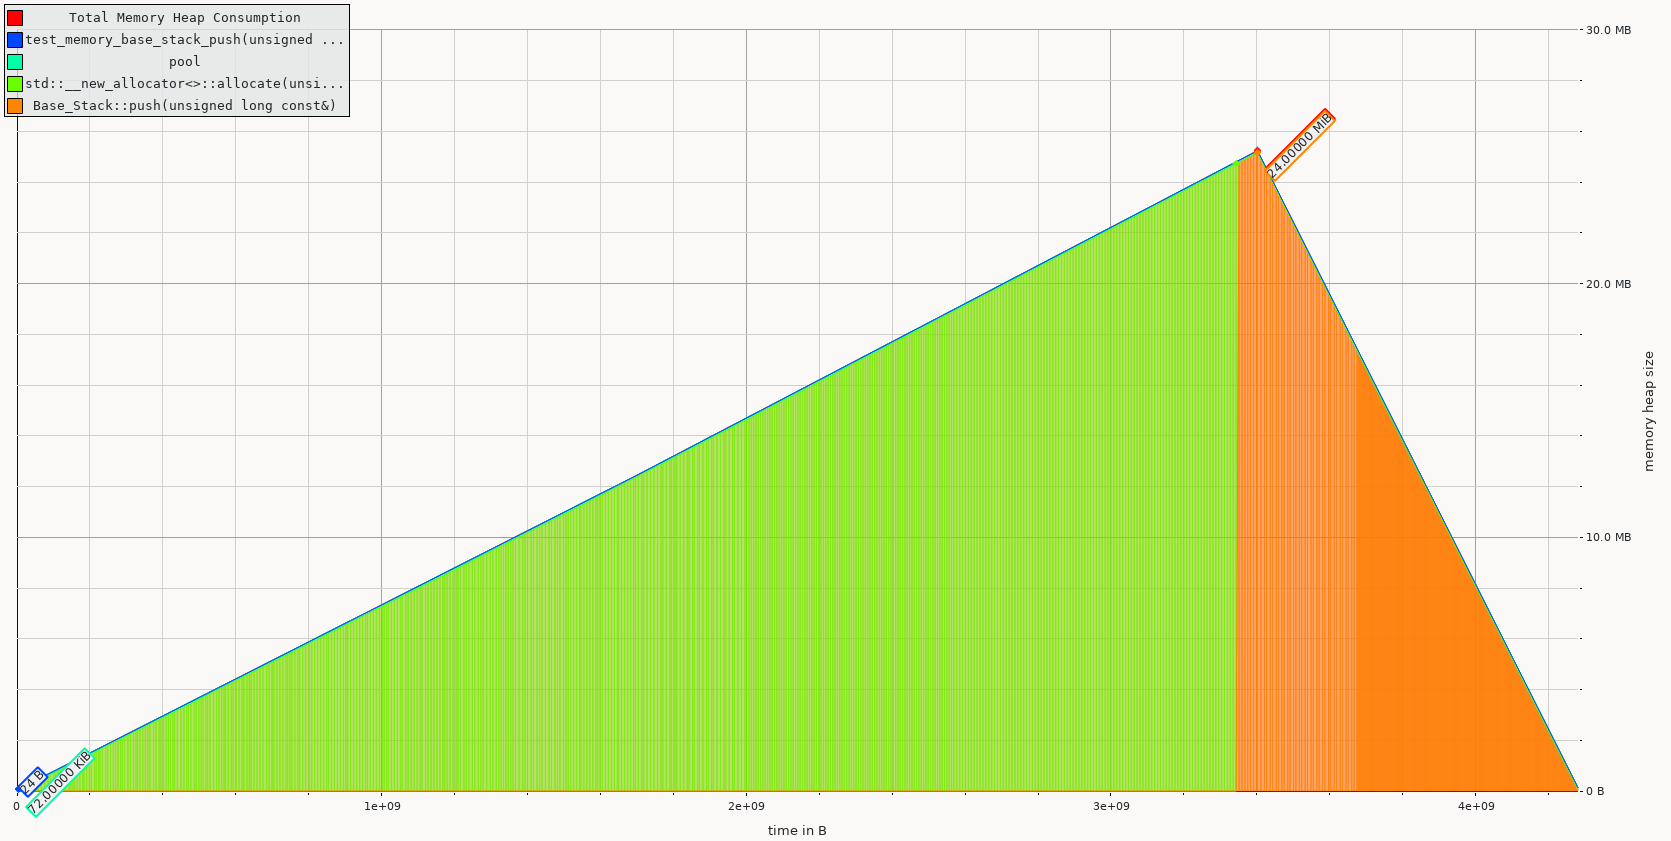
\includegraphics[width=1.0\textwidth]{../../resources/memory_consumption_of_solver3_benchmark_memory_base_stack_with_list_2.png}
  \caption{\texttt{./results/massif_solver3_benchmark_memory_base_stack_for_latex_2.out}}
\end{figure}

Подробнее из пика (снимок \(N = 465\)):
\begin{lstlisting}[caption={}, label={}, style=style_code_block]
->59.88% (25,165,824B) 0x109610: Base_Stack::push(unsigned long const&) (base_stack.hpp:11)
  ->58.96% (24,778,752B) 0x1093FC: test_memory_base_stack_push(unsigned long, unsigned long) (benchmark_memory_base_stack.cpp:43)
  | ->58.96% (24,778,752B) 0x10953E: main (benchmark_memory_base_stack.cpp:59)
  |   
  ->00.92% (387,072B) 0x1094BB: test_memory_base_stack_push(unsigned long, unsigned long) (benchmark_memory_base_stack.cpp:51)
    ->00.92% (387,072B) 0x10953E: main (benchmark_memory_base_stack.cpp:59)

>00.00% (24B) 0x109357: test_memory_base_stack_push(unsigned long, unsigned long) (benchmark_memory_base_stack.cpp:35)
  ->00.00% (24B) 0x10953E: main (benchmark_memory_base_stack.cpp:59)
\end{lstlisting}
Тогда 
\begin{dmath*}
  S'_h = 25165824 + 24 = 25165848 \text{ байт}
\end{dmath*}
и 
\begin{dmath*}
  \Delta_h = S_h - S'_h =  25167432 - 25165824 + 24 = 1584 \text{ байт}
\end{dmath*}


Аналогичные расчёты и змаеры можно провести для других базовых стеков. 
\begin{mdframed}[style=mdfStyleCode]%
  \begin{remark}\rm%
    Проводить измерения со стеками, построенными на структурах, которые выделяют память с запасом, стоит очень внимательно. Так, например, \texttt{std::vector} выделяет память с запасом, например, при помещении в него \(17\) элементов типа \texttt{size_t} он, скорее всего, будет занимать памяти, как будто в нём \(32\) элемента. См. \texttt{size}, \texttt{capacity}.
\end{remark}
\end{mdframed}

\subsection{\texttt{Base_Stack} на \texttt{std::forward_list}}

Рассмотрим последний пример для \texttt{std::forward_list}. Это односвязный список. 
\begin{mdframed}[style=mdfStyleCode]%
  \begin{remark}\rm%
  Его нельзя по умолчанию использовать как шаблонный параметр для \texttt{std::stack}, поскольку названия его методов отличаются от тех, что требуются. Однако мы можем самостоятельно написать нужные нам четыре метода \texttt{stack} с использованием методов \texttt{forward_list} напрямую. 
\end{remark}
\end{mdframed}


\begin{minted}[breaklines=true]{cpp}
#include <forward_list>
using elem_t = size_t;

class Base_Stack {
public:
  std::forward_list<elem_t> stack;

  void push(const elem_t &value) { stack.push_front(value); }
  bool empty() { return stack.empty(); }

  elem_t pop() {
    elem_t element = stack.front();
    stack.pop_front();
    return element;
  }

  elem_t top() { return stack.front(); }
};
\end{minted}

Для \texttt{Stack}
\begin{figure}[H]
  \centering
  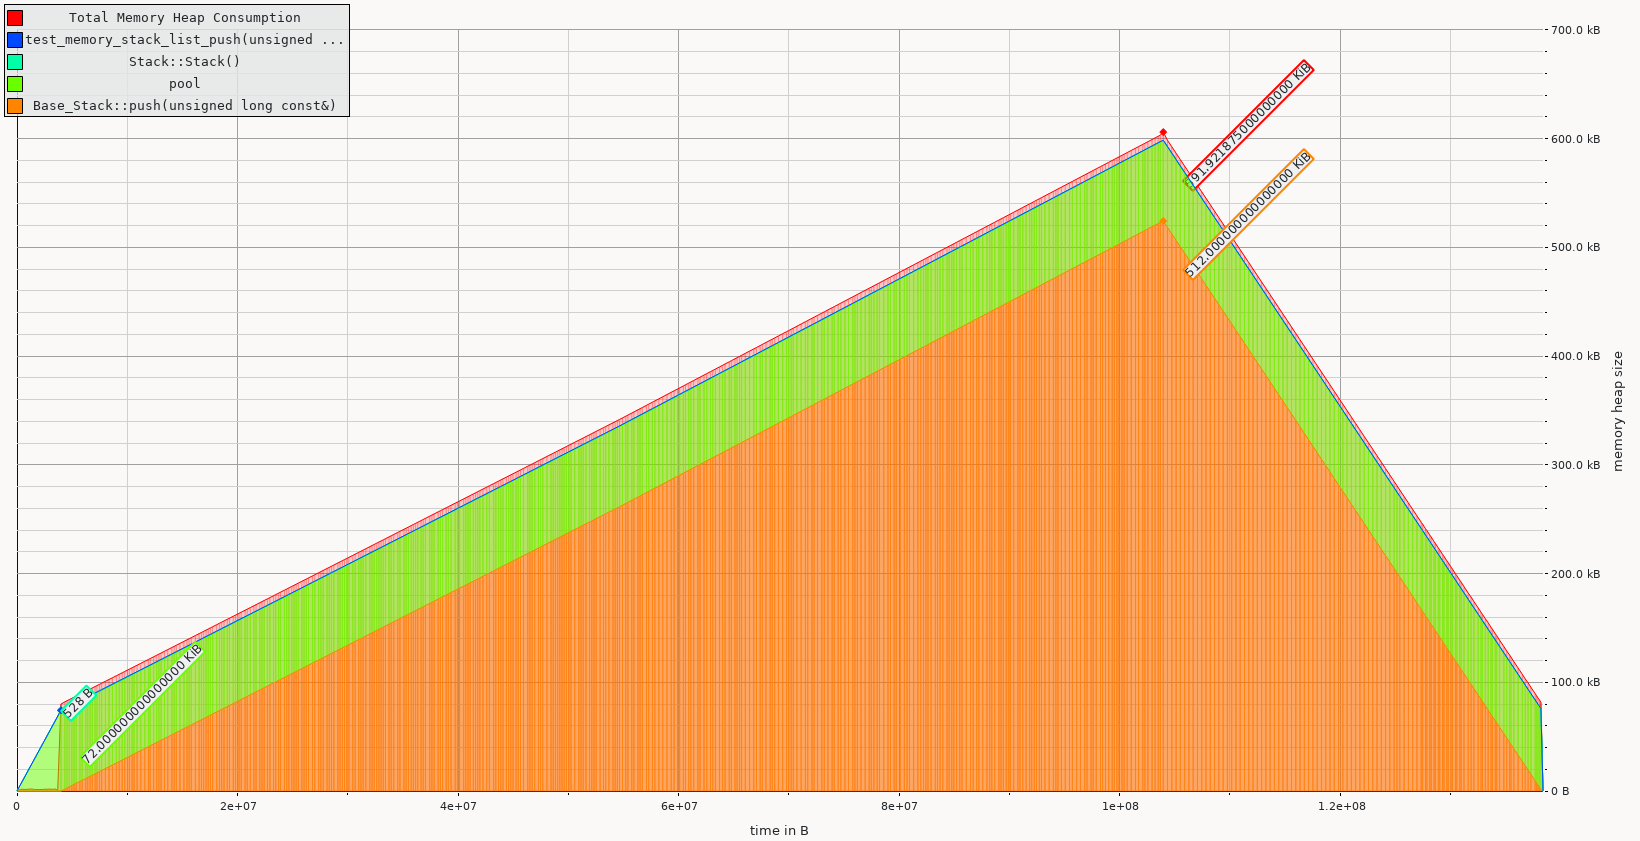
\includegraphics[width=1.0\textwidth]{../../resources/memory_consumption_of_solver3_benchmark_memory_stack_with_forward_list_1.png}
  \caption{\texttt{./results/massif_solver3_benchmark_memory_stack_for_latex_3.out}}
\end{figure}
Пик при \(N = 396\):
\begin{lstlisting}[caption={}, label={}, style=style_code_block]
->60.38% (524,288B) 0x10A281: std::forward_list<unsigned long, std::allocator<unsigned long> >::push_front(unsigned long const&) (forward_list.h:880)
  ->60.38% (524,288B) 0x10A15A: Base_Stack::push(unsigned long const&) (base_stack.hpp:9)
    ->60.31% (523,664B) 0x109EB7: Stack::push(unsigned long) (solution.cpp:33)
    | ->60.31% (523,664B) 0x1093DC: test_memory_stack_list_push(unsigned long, unsigned long) (benchmark_memory_stack.cpp:43)
    |   ->60.31% (523,664B) 0x109549: main (benchmark_memory_stack.cpp:60)
    |     
    ->00.05% (448B) 0x109F29: Stack::push(unsigned long) (solution.cpp:43)
    | ->00.05% (448B) 0x1093DC: test_memory_stack_list_push(unsigned long, unsigned long) (benchmark_memory_stack.cpp:43)
    |   ->00.05% (448B) 0x109549: main (benchmark_memory_stack.cpp:60)
    |     
    ->00.02% (176B) 0x109F55: Stack::push(unsigned long) (solution.cpp:49)
      ->00.02% (176B) 0x1093DC: test_memory_stack_list_push(unsigned long, unsigned long) (benchmark_memory_stack.cpp:43)
        ->00.02% (176B) 0x109549: main (benchmark_memory_stack.cpp:60)
          

->00.06% (528B) 0x109C98: Stack::Stack() (solution.cpp:4)
| ->00.06% (528B) 0x10935C: test_memory_stack_list_push(unsigned long, unsigned long) (benchmark_memory_stack.cpp:35)
|   ->00.06% (528B) 0x109549: main (benchmark_memory_stack.cpp:60)
|     
->00.00% (40B) 0x10934B: test_memory_stack_list_push(unsigned long, unsigned long) (benchmark_memory_stack.cpp:35)
  ->00.00% (40B) 0x109549: main (benchmark_memory_stack.cpp:60)
\end{lstlisting}
Откуда видно, что \(n \cdot S_5 =524288\) байт, на \((B + 1)\cdot S_3 + S_4\) потребовалось \(528\), а на \(4\cdot S_1 + S_2\) потребовалось \(40\) байт.
Итого
\begin{dmath*}
  S_h = 524288 + 568 = 524856 \text{ байт.}
\end{dmath*}

Рассмотрим \texttt{Base_Stack}:
\begin{figure}[H]
  \centering
  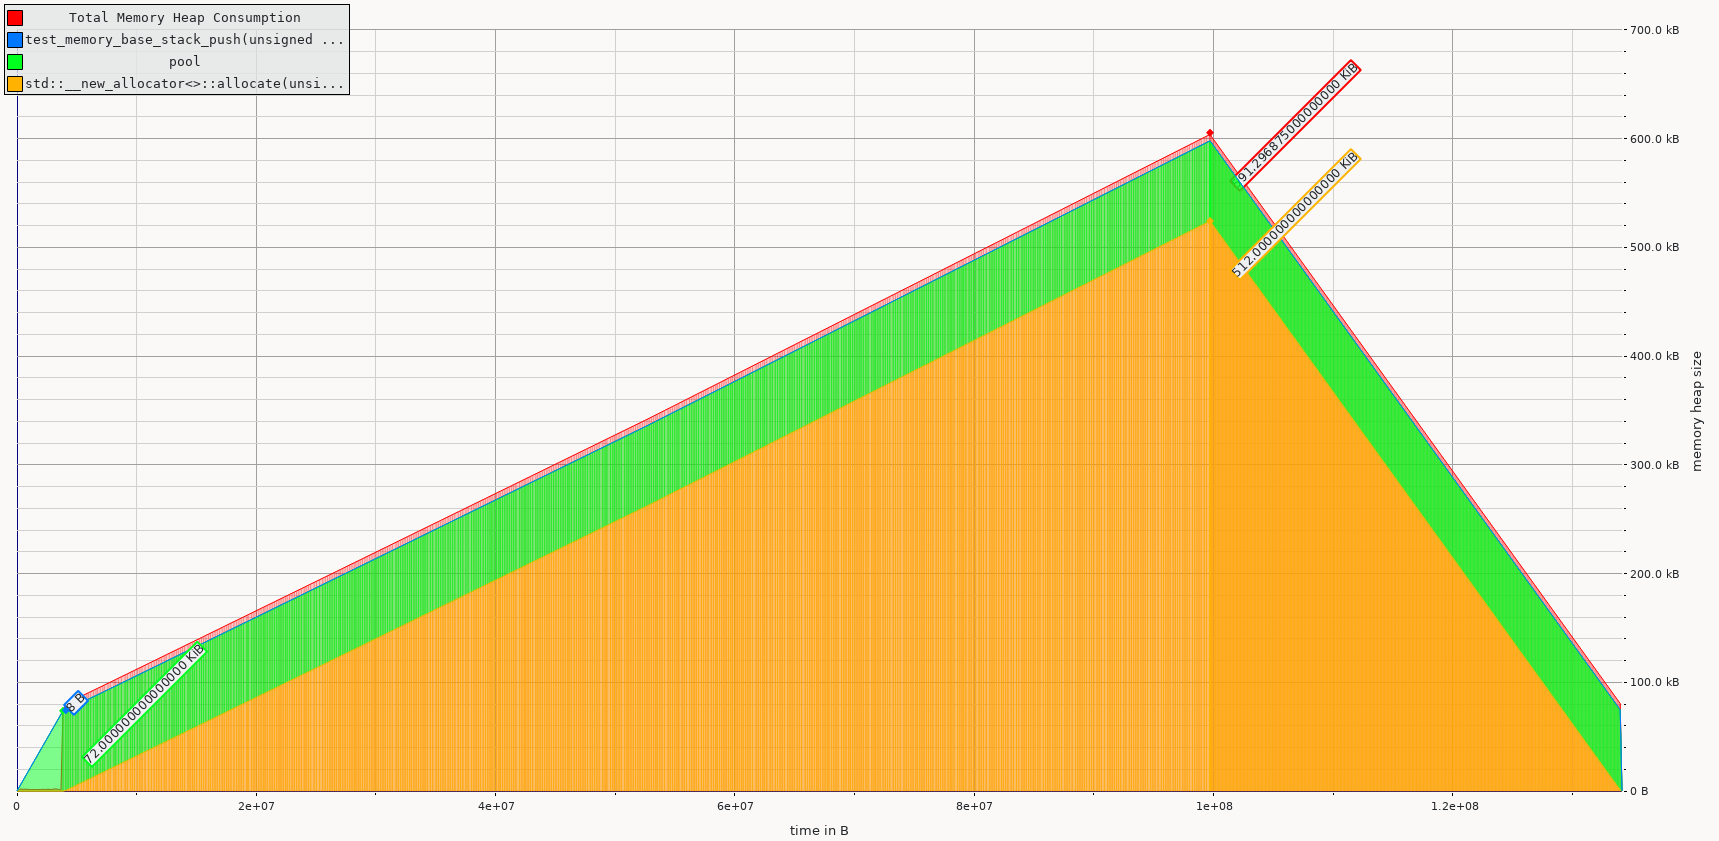
\includegraphics[width=1.0\textwidth]{../../resources/memory_consumption_of_solver3_benchmark_memory_base_stack_with_forward_list_1.png}
  \caption{\texttt{./results/massif_solver3_benchmark_memory_base_stack_for_latex_3.out}}
\end{figure}
Пик при \(N = 510\):
\begin{lstlisting}[caption={}, label={}, style=style_code_block]
->60.54% (524,288B) 0x109679: std::forward_list<unsigned long, std::allocator<unsigned long> >::push_front(unsigned long const&) (forward_list.h:880)
  ->60.54% (524,288B) 0x109598: Base_Stack::push(unsigned long const&) (base_stack.hpp:9)
    ->60.54% (524,288B) 0x1093D7: test_memory_base_stack_push(unsigned long, unsigned long) (benchmark_memory_base_stack.cpp:43)
      ->60.54% (524,288B) 0x109515: main (benchmark_memory_base_stack.cpp:59)
        

->00.00% (8B) 0x109337: test_memory_base_stack_push(unsigned long, unsigned long) (benchmark_memory_base_stack.cpp:35)
  ->00.00% (8B) 0x109515: main (benchmark_memory_base_stack.cpp:59)
\end{lstlisting}
Мы видим, что на \texttt{push} было потрачено \(524288\) байт, то есть для добавления одного элемента требуется \(S_5 = 524288/2^{15} = 16\) байта. (Действительно, поскольку \texttt{std::forward_list} -- это односвязный список и его нода имеет один указатель и элемент данных). 

Пустой же \texttt{Base_Stack} после инициализации занимает 
\begin{lstlisting}[caption={}, label={}, style=style_code_block]
->00.00% (8B) 0x109337: test_memory_base_stack_push(unsigned long, unsigned long) (benchmark_memory_base_stack.cpp:35)
  ->00.00% (8B) 0x109515: main (benchmark_memory_base_stack.cpp:59)
\end{lstlisting}
ровно \(8\) байт, то есть в наших обозначениях \(S_3 = 8\).

Таким образом, 
\begin{dmath*}
  S'_h = 524288 + 8 = 524296 
\end{dmath*}
тогда
\begin{dmath*}
  \Delta_h = S_h - S'_h = 524856 - 524296  = 560 
\end{dmath*}
или по формуле (\dref{5}): \(48 + 64\cdot 8 = 560\).


\section{Результаты}

В этой немного затянувшейся работе мы смогли решить поставленную задачу. А также при помощи различных инструментов подтвердить свои теоретические выкладки.

Аналогично данной задаче можно решить задачу с построением стека с дополнительным методом \texttt{min()}.